\documentclass[a4paper,12pt]{article}
% \usepackage[utf8]{vietnam}
\usepackage{geometry}
\usepackage{amsmath,amsfonts,amssymb}
\usepackage{graphicx}
\usepackage{float}
\usepackage{subcaption}
\usepackage{caption}
\usepackage{booktabs}
\usepackage{longtable}
\usepackage{hyperref}
\hypersetup{hidelinks}
\usepackage{enumitem}
\usepackage{xcolor}
\usepackage{titling}
\usepackage{fancyhdr}
\usepackage{parskip}
\usepackage{titling}
\usepackage{listings}
\usepackage{tikz}
\usetikzlibrary{arrows.meta,positioning}

% Keep figures within the text area and allow them to share pages with prose.
\setkeys{Gin}{height=0.60\textheight,keepaspectratio}
\renewcommand{\topfraction}{0.88}
\renewcommand{\bottomfraction}{0.75}
\renewcommand{\textfraction}{0.10}
\renewcommand{\floatpagefraction}{0.85}
\setcounter{topnumber}{3}
\setcounter{bottomnumber}{2}
\setcounter{totalnumber}{4}
\setlength{\textfloatsep}{10pt plus 2pt minus 3pt}
\setlength{\floatsep}{8pt plus 2pt minus 2pt}
\setlength{\intextsep}{8pt plus 2pt minus 2pt}
\makeatletter
\setlength{\@fptop}{0pt}
\setlength{\@fpsep}{3pt}
\setlength{\@fpbot}{0pt}
\makeatother
\captionsetup{font=small,skip=5pt}
\renewcommand{\arraystretch}{1.12}

% Custom colors
\definecolor{titleblue}{RGB}{0,102,204}
\definecolor{headingblue}{RGB}{0,51,102}

% Code listing style
\lstset{
    language=Python,
    basicstyle=\ttfamily\small,
    keywordstyle=\color{blue}\bfseries,
    stringstyle=\color{purple},
    commentstyle=\color{gray}\itshape,
    numberstyle=\tiny,
    numbers=left,
    stepnumber=1,
    numbersep=5pt,
    showspaces=false,
    showstringspaces=false,
    frame=single,
    breaklines=true,
    breakatwhitespace=true,
    tabsize=4
}


% Page layout
\geometry{top=2.5cm,bottom=2.5cm,left=2.5cm,right=2.5cm}
\setlength{\parindent}{0pt}
\setlength{\parskip}{1em}

% Header and footer
\pagestyle{fancy}
\fancyhf{}
\fancyhead[L]{\textbf{INS3155 - Computer Vision Midterm Report}}
\fancyhead[R]{}
\setlength{\headheight}{15pt}
\fancyfoot[C]{\thepage}

% Title customization
\pretitle{\centering\LARGE\bfseries}
\posttitle{\vspace{0.5cm}}

\preauthor{\centering}
\postauthor{}
\predate{\centering}
\postdate{}


% Custom colors
\definecolor{titleblue}{RGB}{0,102,204}
\definecolor{headingblue}{RGB}{0,51,102}

\begin{document}

\title{\textcolor{titleblue}{Midterm Project Report}\kern-1pt}

\author{\parbox{0.45\linewidth}{\centering
Name: Do Nam Hai\\
Student ID: 23070846\\
Email: 23070846@vnu.edu.vn}}

\date{\today}

% \date{Ngày nộp: May 03, 2025}

\maketitle

\begin{abstract}
This project evaluates classical image-processing methods for denoising, stereo reconstruction, and four-image panorama stitching. Mean, Gaussian, and median filters with Laplacian sharpening were compared on synthetic Gaussian and salt-and-pepper noise using PSNR, SSIM, MSE, and runtime. Gaussian filtering achieved the highest selected PSNR for Gaussian noise, while a $3\times3$ median filter performed best for impulse noise; sharpening gains depended on configuration. On the rectified Venus pair, SGBM provided higher valid-disparity coverage and lower ground-truth disparity error than BM across tested settings, with greater runtime. Reconstructed point clouds use an assumed camera model and therefore show qualitative normalized depth only. For stitching, SIFT, ORB, and AKAZE were evaluated with RANSAC homographies and feather blending; SIFT had the lowest selected pooled reprojection error, while ORB showed greater corner sensitivity. The results reveal trade-offs among fidelity, coverage, speed, and geometric stability.
\end{abstract}

\section{Introduction}
Image filtering, stereo reconstruction, and image stitching address three practical problems in computer vision: improving image quality, recovering scene structure, and combining overlapping views. Noise can obscure fine details, uncertain correspondences can distort reconstructed geometry, and inaccurate alignment can produce visible seams in a panorama. Traditional computer vision provides explicit methods for these tasks through local filtering, feature matching, and geometric estimation. Their parameters and intermediate outputs make it possible to examine how processing choices affect both numerical measurements and visible image quality.

This project investigates these methods in three parts. Part A compares mean, Gaussian, and median filtering under Gaussian and salt-and-pepper noise, followed by Laplacian sharpening to examine the balance between noise removal and detail enhancement. Part B studies stereo correspondences, fundamental matrix estimation, and disparity computation using Block Matching (BM) and Semi-Global Block Matching (SGBM), with attention to the camera assumptions required for 3D reconstruction. Part C compares feature detectors and descriptors in a pipeline that matches, aligns, and blends four overlapping images into a panorama. Each part presents the methodology, implementation and results, and comparative analysis. Quantitative measurements and visual comparisons are used together to assess accuracy, runtime, and failure cases, followed by the overall conclusions and possible improvements.

\section{Part A: Image Filtering}
\label{sec:part-a}
\subsection{Methodology}

\textbf{Reference image and processing workflow.}\par
The input is \texttt{succulent\_20231108\_171619.jpg}, a photograph containing succulent leaves, fine gravel, a glazed pot, and a broad background. Its encoded dimensions are $4128\times3096$ pixels. Correcting EXIF orientation 6 produces a $3096\times4128$ RGB image, which is resized to $768\times1024$ using OpenCV's \texttt{INTER\_AREA}. No crop is applied to the reference, and the original JPEG is preserved. The available metadata records the original filename and local path but does not identify the photographer or usage terms; whether the image was self-captured could not be verified. All quality measurements use this resized image before synthetic corruption as the reference.

\begin{center}
\small
\fbox{EXIF correction, RGB conversion, and area resize}\\[5pt]
$\downarrow$\\[5pt]
\fbox{Gaussian or salt-and-pepper noise}\\[5pt]
$\downarrow$\\[5pt]
\fbox{Mean, Gaussian, or median denoising}\\[5pt]
$\downarrow$\\[5pt]
\fbox{Scaled Laplacian sharpening}\\[5pt]
$\downarrow$\\[5pt]
\fbox{PSNR, SSIM, MSE, and processing time}
\end{center}
A separate control sharpens the noisy image directly. Both the denoised and sharpened outputs are evaluated against the same reference.

\textbf{Noise models.}\par
Gaussian noise consists of independent zero-mean samples added to each RGB element, with standard deviation $\sigma_n\in\{10,20,30\}$ in 8-bit intensity units:
\begin{equation}
N_G=\operatorname{round}\!\left[\operatorname{clip}_{[0,255]}(I+\epsilon)\right],
\qquad \epsilon\sim\mathcal{N}(0,\sigma_n^2).
\end{equation}
Addition uses floating-point values. Clipping and rounding can change the realized noise distribution, so its measured mean and standard deviation are retained in the run manifest.

Salt-and-pepper noise selects $\operatorname{round}(pHW)$ distinct spatial pixels. The tested densities are $p\in\{0.01,0.03,0.05\}$. Approximately half are set to white and half to black across all channels. The selected fraction and the fraction whose values actually change are recorded separately. Seeds 42, 43, and 44 are fixed; random-stream identity also includes the noise type and level. Every method receives the same corrupted image for each noise condition and seed.

\textbf{Denoising and sharpening.}\par
For a $k\times k$ neighbourhood $\Omega_k$, the mean filter is
\begin{equation}
D_M(x,y,c)=\frac{1}{k^2}\sum_{(u,v)\in\Omega_k}N(x+u,y+v,c).
\end{equation}
The Gaussian filter uses a finite normalized kernel:
\begin{equation}
G(u,v)=\frac{\exp[-(u^2+v^2)/(2\sigma_f^2)]}
{\sum_{(a,b)\in\Omega_k}\exp[-(a^2+b^2)/(2\sigma_f^2)]},
\qquad D_G=G*N.
\end{equation}
The median filter replaces each channel value with the median of its neighbourhood. These operations use \texttt{cv2.blur}, \texttt{cv2.GaussianBlur}, and \texttt{cv2.medianBlur}, independently per channel. Replicated borders are used throughout, including the median filter's native border handling.\footnote{OpenCV filtering API: \url{https://docs.opencv.org/4.x/d4/d86/group__imgproc__filter.html}.}

Laplacian enhancement follows denoising in the main pipeline:
\begin{equation}
J=\operatorname{round}\!\left[\operatorname{clip}_{[0,255]}
\left(D-\alpha s_k\Delta_kD\right)\right],
\qquad s_k=2^{4-2k}.
\label{eq:a-sharpening}
\end{equation}
The derivative is computed with \texttt{cv2.Laplacian} in float32 to preserve its sign. Apertures $k\in\{3,5,7\}$ use scales $1/4$, $1/64$, and $1/1024$ to control derivative gain across apertures. The strength is $\alpha\in\{0.1,0.2,0.25,0.5\}$. Sharpening enhances local contrast and is assessed separately from noise removal.\footnote{\raggedright OpenCV Laplace operator: \url{https://docs.opencv.org/4.x/d5/db5/tutorial_laplace_operator.html}.}

\textbf{Quality metrics and runtime.}\par
For $N=3HW$ RGB elements, the reference $I$ and result $J$ are compared using
\begin{equation}
\operatorname{MSE}=\frac{1}{N}\sum_{i=1}^{N}(I_i-J_i)^2,
\qquad
\operatorname{PSNR}=10\log_{10}\frac{255^2}{\operatorname{MSE}}.
\end{equation}
Differences and squares use float64 to avoid unsigned-integer overflow. MSE is reported in squared 8-bit intensity units. Zero MSE gives infinite PSNR. SSIM measures local luminance, contrast, and structure:
\begin{equation}
\operatorname{SSIM}(x,y)=
\frac{(2\mu_x\mu_y+C_1)(2\sigma_{xy}+C_2)}
{(\mu_x^2+\mu_y^2+C_1)(\sigma_x^2+\sigma_y^2+C_2)},
\end{equation}
where $C_1=(0.01\cdot255)^2$ and $C_2=(0.03\cdot255)^2$. The implementation uses \texttt{data\_range=255}, \texttt{channel\_axis=-1}, Gaussian window weights with sigma 1.5, and population covariance. Channel scores are averaged. The SSIM window sigma is distinct from the filter and noise sigmas.\footnote{scikit-image quality metrics: \url{https://scikit-image.org/docs/stable/api/skimage.metrics.html\#skimage.metrics.structural_similarity}.}

Quality is reported as mean $\pm$ sample standard deviation over three seeds; PSNR is averaged in dB. Each processed case has two warm-ups and ten timed repetitions per seed. A configuration's runtime is the median of its 30 samples, with interquartile range (IQR) in parentheses. Timing includes processing checks and array conversions, and excludes noise generation, metric computation, disk I/O, and plotting. Denoising--sharpening chains are timed as complete operations. OpenCV uses one thread with OpenCL disabled. No filter runtime is assigned to noisy baselines.

\subsection{Implementation and Results}

\textbf{Experimental setup and parameter grid.}\par
The experiment was implemented with OpenCV, NumPy, Pillow, scikit-image, and Matplotlib. Measurements were collected with Python 3.13.14 on Linux x86\_64 using NumPy 2.5.4, opencv-python-headless 5.0.0.93, Pillow 13.0.0, scikit-image 0.26.0, and Matplotlib 3.11.2. The accompanying reproducibility package records the input checksum, source snapshot, parameters, environment, and realized noise statistics.

The final grid uses denoising kernels $k\in\{3,5,7,9,11\}$ and Gaussian filter sigmas $\sigma_f\in\{0.6,0.8,1.0,1.2,1.4,1.5,1.6\}$. Each of the six noise conditions has 45 denoising settings: five mean, five median, and 35 Gaussian combinations. An earlier coarse, refined, and boundary search covered 382 distinct denoiser configurations and 22 Gaussian sigma values across its searches; it was not a full Cartesian product of those values.

For each noise condition and denoiser family, the highest three-seed mean whole-image PSNR selects the input to sharpening; ties prefer smaller kernels. Each condition then has 36 denoising--sharpening settings and six direct-sharpening controls at $\alpha=0.25$ or $0.5$. Including the six noisy baselines, the experiment contains 528 configuration groups, 1,584 seed-level metric rows, and 15,660 timing samples. All 528 seed-42 cases are saved as PNG files along with the reference. The accompanying machine-readable results retain every tested setting, including poorly performing configurations.

\textbf{Noisy baselines and denoising results.}\par
Table~\ref{tab:a-baselines} reports the corrupted-reference baselines. Tables~\ref{tab:a-gaussian} and~\ref{tab:a-impulse} compare the PSNR-selected configuration within each denoiser family. Appendix~\ref{app:a-full} reports every configuration in the final grid; the machine-readable results retain the full precision and individual seeds.
\begin{table}[htbp]
\centering
\small
\setlength{\tabcolsep}{3pt}
\caption{Noisy baselines. Gaussian levels denote noise standard deviation; impulse levels denote the fraction of selected pixels. Quality is mean $\pm$ sample standard deviation over three seeds.}
\label{tab:a-baselines}
\begin{tabular}{llrrr}
\toprule
\multicolumn{1}{c}{Noise} & \multicolumn{1}{c}{Level} & \multicolumn{1}{c}{PSNR (dB)} & \multicolumn{1}{c}{SSIM} & \multicolumn{1}{c}{MSE} \\
\midrule
Gaussian & $\sigma_n=10$ & 28.2319 $\pm$ 0.0001 & 0.54723 $\pm$ 0.00010 & 97.70 $\pm$ 0.00 \\
Gaussian & $\sigma_n=20$ & 22.3294 $\pm$ 0.0008 & 0.28528 $\pm$ 0.00013 & 380.31 $\pm$ 0.07 \\
Gaussian & $\sigma_n=30$ & 18.9570 $\pm$ 0.0035 & 0.17793 $\pm$ 0.00011 & 826.76 $\pm$ 0.67 \\
Salt-and-pepper & 1\% & 25.0383 $\pm$ 0.0313 & 0.74063 $\pm$ 0.00112 & 203.82 $\pm$ 1.47 \\
Salt-and-pepper & 3\% & 20.2892 $\pm$ 0.0058 & 0.44027 $\pm$ 0.00076 & 608.35 $\pm$ 0.81 \\
Salt-and-pepper & 5\% & 18.0649 $\pm$ 0.0108 & 0.28699 $\pm$ 0.00171 & 1015.29 $\pm$ 2.52 \\
\bottomrule
\end{tabular}
\end{table}
\begin{table}[htbp]
\centering
\small
\setlength{\tabcolsep}{1.9pt}
\caption{Gaussian-noise denoising comparison. Quality is mean $\pm$ sample standard deviation; time is median (IQR), in milliseconds. The filter sigma is $\sigma_f$.}
\label{tab:a-gaussian}
\begin{tabular}{llrrrr}
\toprule
\multicolumn{1}{c}{Noise level} & \multicolumn{1}{c}{Filter} & \multicolumn{1}{c}{PSNR (dB)} & \multicolumn{1}{c}{SSIM} & \multicolumn{1}{c}{MSE} & \multicolumn{1}{c}{Time (ms)} \\
\midrule
10 & G $5\times 5$, $\sigma_f=0.8$ & 34.2954 $\pm$ 0.0021 & 0.87793 $\pm$ 0.00003 & 24.18 $\pm$ 0.01 & 0.974 (0.294) \\
10 & M $3\times 3$ & 33.7557 $\pm$ 0.0018 & 0.87724 $\pm$ 0.00005 & 27.38 $\pm$ 0.01 & 0.422 (0.037) \\
10 & Med $3\times 3$ & 33.5676 $\pm$ 0.0021 & 0.84035 $\pm$ 0.00002 & 28.60 $\pm$ 0.01 & 0.325 (0.050) \\
20 & G $7\times 7$, $\sigma_f=1.2$ & 31.2319 $\pm$ 0.0089 & 0.82511 $\pm$ 0.00014 & 48.97 $\pm$ 0.10 & 2.456 (0.419) \\
20 & M $5\times 5$ & 30.4018 $\pm$ 0.0064 & 0.83307 $\pm$ 0.00013 & 59.28 $\pm$ 0.09 & 0.532 (0.041) \\
20 & Med $5\times 5$ & 30.6926 $\pm$ 0.0124 & 0.79309 $\pm$ 0.00037 & 55.44 $\pm$ 0.16 & 3.226 (0.542) \\
30 & G $9\times 9$, $\sigma_f=1.5$ & 29.4227 $\pm$ 0.0033 & 0.79417 $\pm$ 0.00018 & 74.27 $\pm$ 0.06 & 3.045 (0.677) \\
30 & M $5\times 5$ & 28.9585 $\pm$ 0.0025 & 0.75971 $\pm$ 0.00012 & 82.65 $\pm$ 0.05 & 0.540 (0.032) \\
30 & Med $7\times 7$ & 29.0048 $\pm$ 0.0118 & 0.77319 $\pm$ 0.00042 & 81.77 $\pm$ 0.22 & 60.777 (3.619) \\
\bottomrule
\end{tabular}
\end{table}
\begin{table}[htbp]
\centering
\small
\setlength{\tabcolsep}{2pt}
\caption{Salt-and-pepper denoising comparison. Quality is mean $\pm$ sample standard deviation; time is median (IQR), in milliseconds. The filter sigma is $\sigma_f$.}
\label{tab:a-impulse}
\begin{tabular}{llrrrr}
\toprule
\multicolumn{1}{c}{Density} & \multicolumn{1}{c}{Filter} & \multicolumn{1}{c}{PSNR (dB)} & \multicolumn{1}{c}{SSIM} & \multicolumn{1}{c}{MSE} & \multicolumn{1}{c}{Time (ms)} \\
\midrule
1\% & G $5\times 5$, $\sigma_f=1.0$ & 32.6387 $\pm$ 0.0243 & 0.87682 $\pm$ 0.00011 & 35.42 $\pm$ 0.20 & 1.149 (0.470) \\
1\% & M $3\times 3$ & 32.1472 $\pm$ 0.0257 & 0.85450 $\pm$ 0.00016 & 39.66 $\pm$ 0.24 & 0.417 (0.038) \\
1\% & Med $3\times 3$ & 38.2479 $\pm$ 0.0093 & 0.96514 $\pm$ 0.00002 & 9.73 $\pm$ 0.02 & 0.324 (0.024) \\
3\% & G $7\times 7$, $\sigma_f=1.4$ & 30.1131 $\pm$ 0.0131 & 0.81756 $\pm$ 0.00053 & 63.35 $\pm$ 0.19 & 2.725 (1.215) \\
3\% & M $5\times 5$ & 29.5823 $\pm$ 0.0088 & 0.80084 $\pm$ 0.00046 & 71.59 $\pm$ 0.14 & 0.628 (0.908) \\
3\% & Med $3\times 3$ & 37.8470 $\pm$ 0.0330 & 0.96393 $\pm$ 0.00006 & 10.68 $\pm$ 0.08 & 0.449 (0.347) \\
5\% & G $11\times 11$, $\sigma_f=1.6$ & 28.7862 $\pm$ 0.0185 & 0.79405 $\pm$ 0.00008 & 85.99 $\pm$ 0.37 & 4.042 (1.001) \\
5\% & M $5\times 5$ & 28.3379 $\pm$ 0.0179 & 0.74163 $\pm$ 0.00012 & 95.34 $\pm$ 0.39 & 0.683 (0.194) \\
5\% & Med $3\times 3$ & 37.4485 $\pm$ 0.0597 & 0.96265 $\pm$ 0.00003 & 11.70 $\pm$ 0.16 & 0.437 (0.166) \\
\bottomrule
\end{tabular}
\end{table}
\begin{figure}[htbp]
\centering
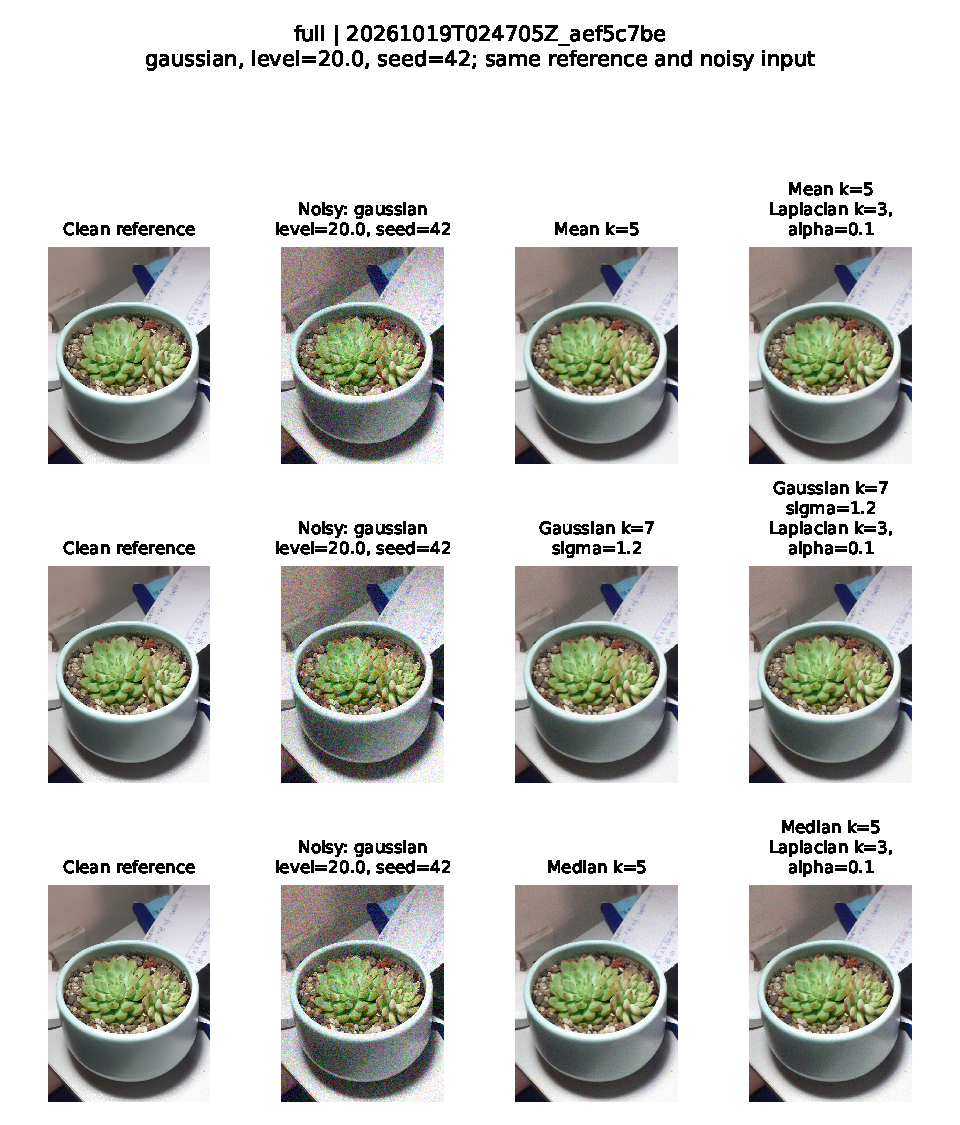
\includegraphics[width=0.98\textwidth,trim=0 15pt 0 90pt,clip]{../results/part_a/official/20261019T024705Z_aef5c7be/figures/gaussian_grid.pdf}
\caption{Gaussian noise $\sigma_n=20$, seed 42. Rows compare the selected mean, Gaussian, and median denoisers. Columns show original, noisy, denoised, and sharpened images. The fourth column uses illustrative Laplacian $k=3$, $\alpha=0.1$; the selected chains in Table~\ref{tab:a-chains} use separately selected parameters.}
\label{fig:a-gaussian-grid}
\end{figure}
\begin{figure}[htbp]
\centering
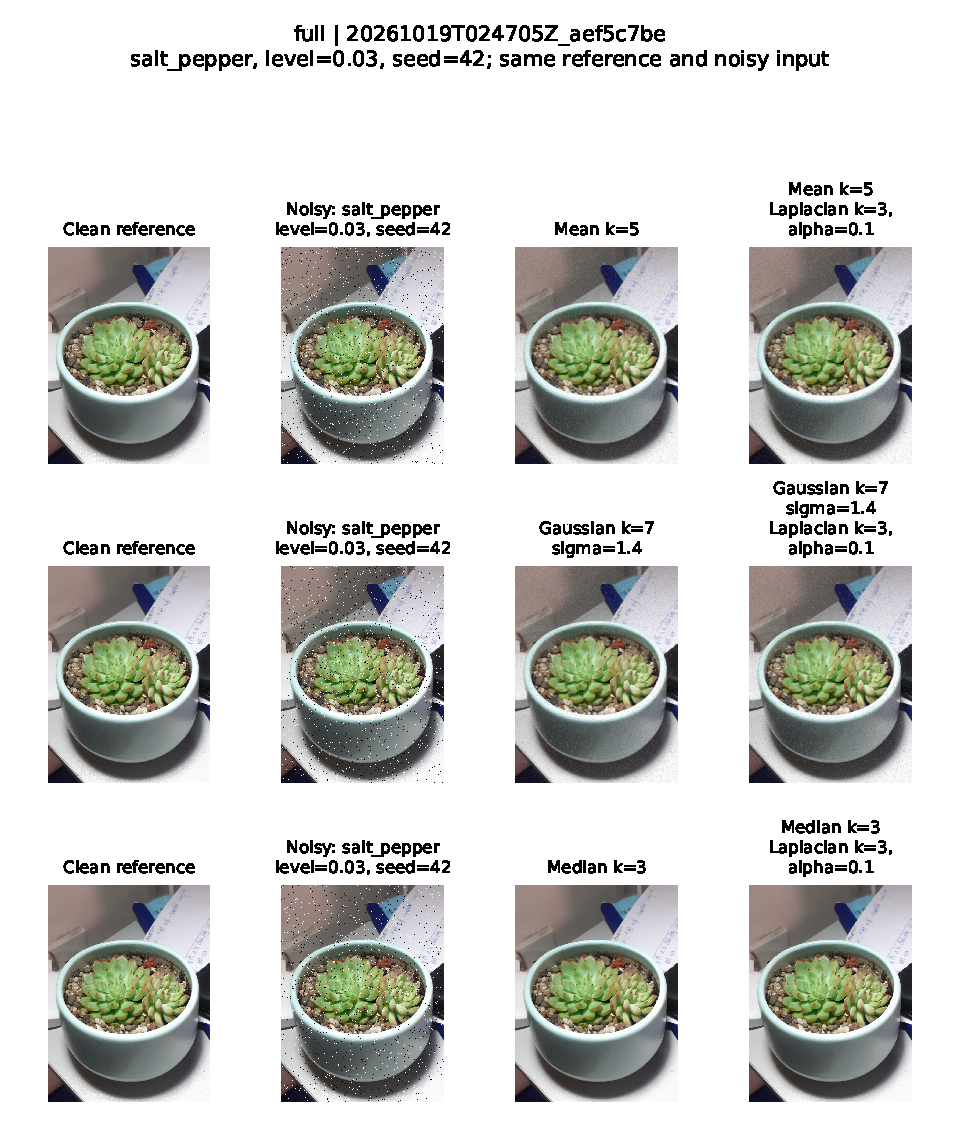
\includegraphics[width=0.98\textwidth,trim=0 15pt 0 90pt,clip]{../results/part_a/official/20261019T024705Z_aef5c7be/figures/salt_pepper_grid.pdf}
\caption{Salt-and-pepper noise $p=3\%$, seed 42, with the same column order and illustrative sharpening parameters as Figure~\ref{fig:a-gaussian-grid}.}
\label{fig:a-impulse-grid}
\end{figure}
\begin{figure}[htbp]
\centering
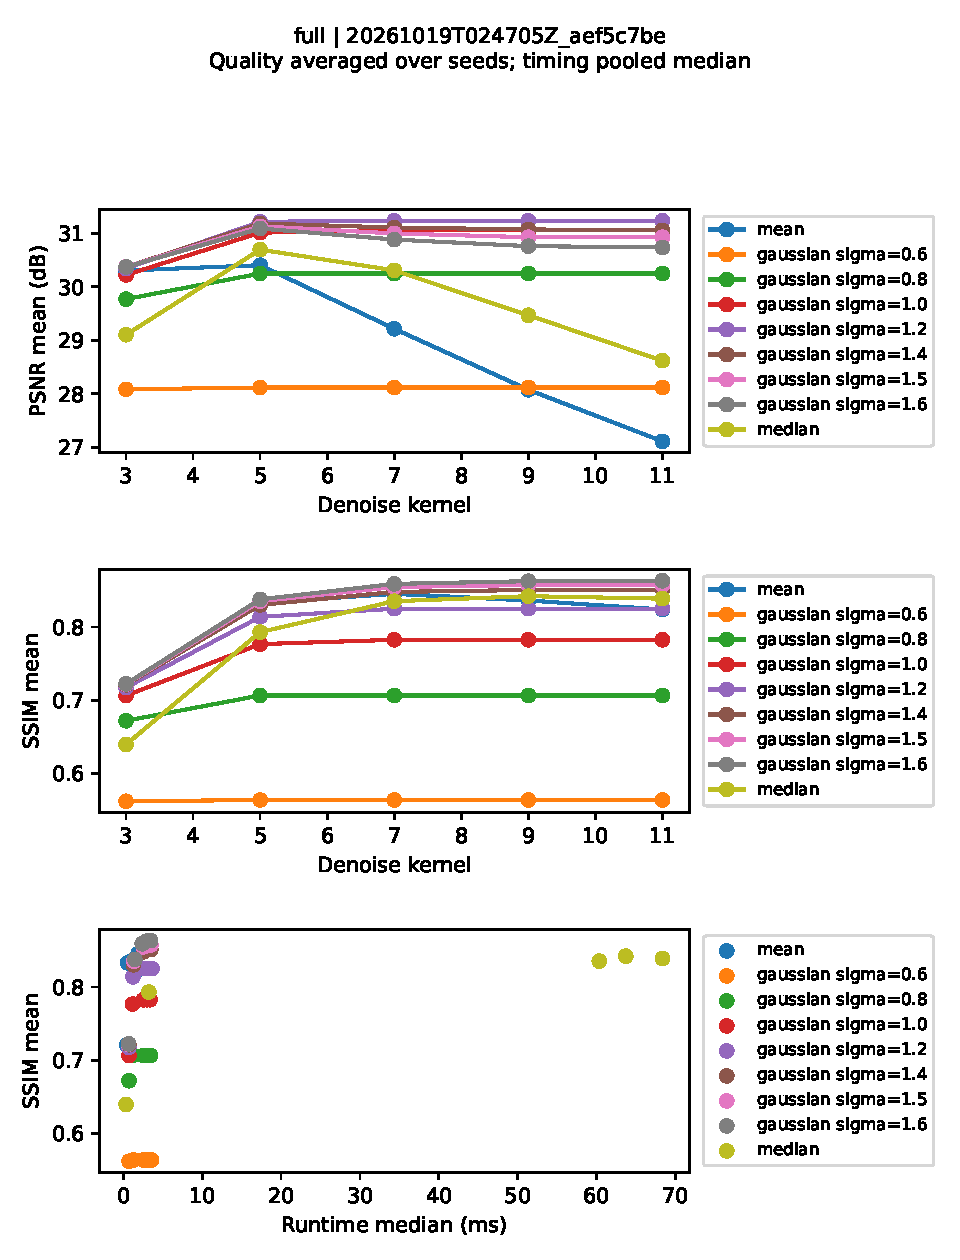
\includegraphics[width=0.68\textwidth,trim=0 0 0 55pt,clip]{../results/part_a/official/20261019T024705Z_aef5c7be/figures/gaussian_sensitivity.pdf}
\caption{Kernel sensitivity and quality/runtime trade-offs at Gaussian noise $\sigma_n=20$. Quality averages the three seeds; time is the pooled median.}
\label{fig:a-sensitivity}
\end{figure}

\textbf{Selected denoising--sharpening chains.}\par
Table~\ref{tab:a-chains} lists the highest mean PSNR at each noise level, selected from the measured denoised outputs and complete sharpening chains. Direct controls are excluded from this selection. The accompanying results package maps each selected configuration to its seed-42 output image and checksum.
\begin{table}[htbp]
\centering
\small
\setlength{\tabcolsep}{2.5pt}
\caption{Selected complete chains. G denotes Gaussian noise (level $\sigma_n$); SP denotes impulse density. Filter sizes are square; Gaussian settings show kernel width / $\sigma_f$. $L$ is the Laplacian aperture. Quality is mean $\pm$ sample standard deviation; time is median (IQR).}
\label{tab:a-chains}
\begin{tabular}{lllrrrr}
\toprule
\multicolumn{1}{c}{Noise} & \multicolumn{1}{c}{Denoiser} & \multicolumn{1}{c}{$L;\alpha$} & \multicolumn{1}{c}{PSNR (dB)} & \multicolumn{1}{c}{SSIM} & \multicolumn{1}{c}{MSE} & \multicolumn{1}{c}{Time (ms)} \\
\midrule
G10 & Gauss 5/.8 & 7; 0.1 & 34.4378 $\pm$ 0.0015 & 0.87848 $\pm$ 0.00002 & 23.40 $\pm$ 0.01 & 11.814 (1.477) \\
G20 & Gauss 7/1.2 & 7; 0.1 & 31.3128 $\pm$ 0.0087 & 0.82536 $\pm$ 0.00014 & 48.06 $\pm$ 0.10 & 12.552 (1.664) \\
G30 & Gauss 9/1.5 & 7; 0.1 & 29.4742 $\pm$ 0.0035 & 0.79435 $\pm$ 0.00017 & 73.39 $\pm$ 0.06 & 12.570 (1.028) \\
SP 1\% & Med 3 & 5; 0.25 & 38.7671 $\pm$ 0.0048 & 0.96794 $\pm$ 0.00002 & 8.64 $\pm$ 0.01 & 9.217 (0.772) \\
SP 3\% & Med 3 & 5; 0.25 & 38.2426 $\pm$ 0.0459 & 0.96655 $\pm$ 0.00006 & 9.75 $\pm$ 0.10 & 12.210 (4.236) \\
SP 5\% & Med 3 & 5; 0.2 & 37.7493 $\pm$ 0.0626 & 0.96474 $\pm$ 0.00004 & 10.92 $\pm$ 0.16 & 12.355 (2.826) \\
\bottomrule
\end{tabular}
\end{table}

The selected chains improve PSNR over their denoised inputs by 0.1423, 0.0809, and 0.0515 dB for Gaussian $\sigma_n=10,20,30$, and by 0.5192, 0.3956, and 0.3009 dB for impulse densities 1\%, 3\%, and 5\%. Gaussian-noise improvements are modest relative to the added cost: at $\sigma_n=20$, the selected denoiser takes 2.456 ms, compared with 12.552 ms for the complete chain. Denoising alone is a reasonable choice when processing speed matters more than this small fidelity gain.

\subsection{Comparative Analysis}

\textbf{Noise removal and edge preservation.}\par
Gaussian filtering gives the highest selected denoising PSNR at all three Gaussian noise levels. At $\sigma_n=20$, Gaussian $7\times7$, $\sigma_f=1.2$ reaches 31.2319 dB, compared with 30.4018 dB for mean $5\times5$ and 30.6926 dB for median $5\times5$. Mean filtering is faster but its equal weighting blurs fine gravel and leaf tips. The PSNR-selected Gaussian setting does not maximize every metric: mean $5\times5$ gives higher SSIM at this level, 0.83307 versus 0.82511.

Median $3\times3$ has the highest selected PSNR and SSIM at every tested impulse density. At 3\%, it increases PSNR from 20.2892 to 37.8470 dB and SSIM from 0.44027 to 0.96393. Its median runtime is 0.449 ms, compared with 2.725 ms for the selected Gaussian filter. Median filtering rejects sparse extrema without spreading them across the neighbourhood. Larger median kernels remove small gravel structures and are unnecessary at these tested densities. Runtime also depends strongly on aperture: the selected median $7\times7$ at Gaussian $\sigma_n=30$ takes 60.777 ms, compared with 3.045 ms for Gaussian $9\times9$, $\sigma_f=1.5$.

\textbf{Smooth regions, texture, and the optimization objective.}\par
Three fixed diagnostic regions cover the pot surface, leaf boundaries, and gravel (Figure~\ref{fig:a-rois}). They use the same coordinates for every method and are not alternative experiment inputs. Whole-image metrics remain the primary selection criterion. The pot surface makes residual grain visible, leaf boundaries expose blur and contrast changes, and gravel exposes fine-texture loss.
\begin{figure}[htbp]
\centering
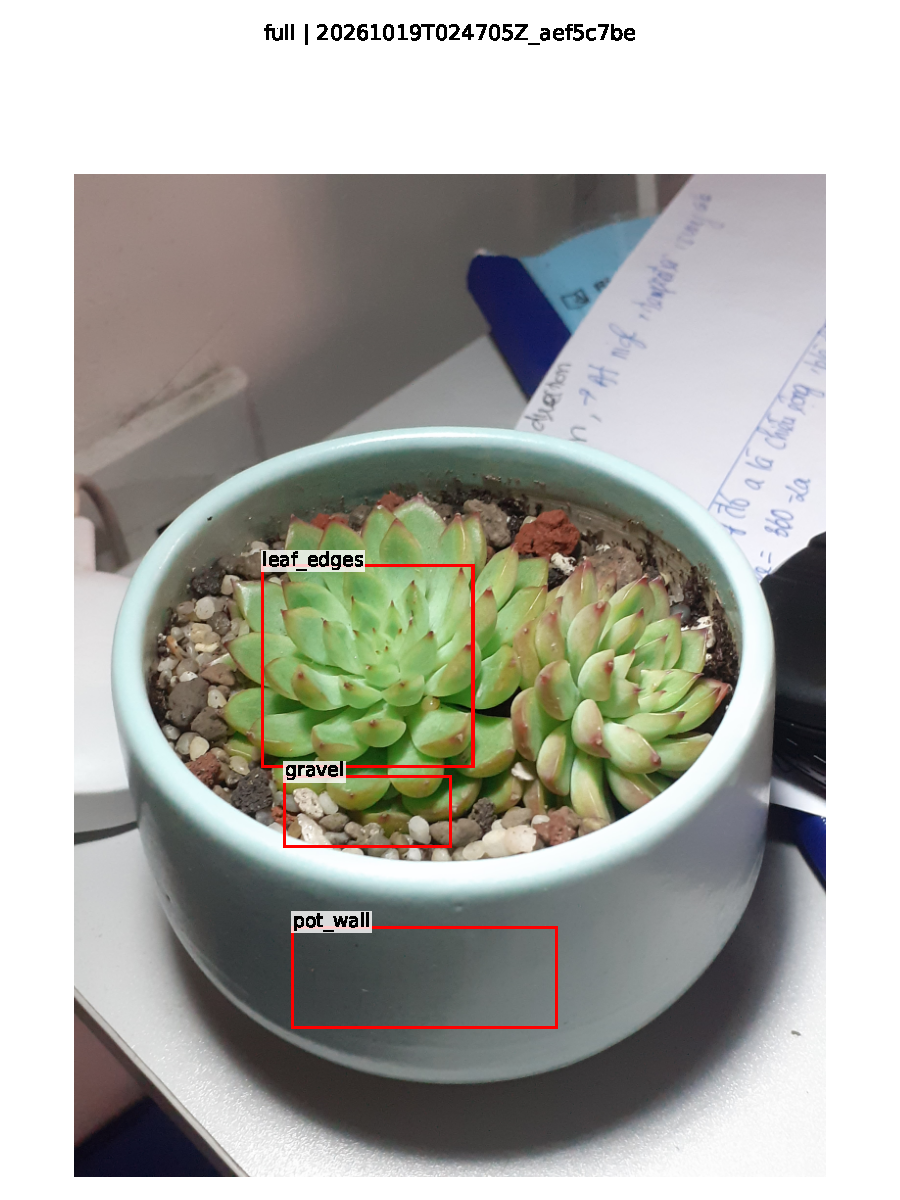
\includegraphics[width=0.54\textwidth,trim=0 70pt 0 58pt,clip]{../results/part_a/official/20261019T024705Z_aef5c7be/figures/reference_rois.pdf}
\caption{Reference image and the three fixed diagnostic regions. The experiment reference remains uncropped.}
\label{fig:a-rois}
\end{figure}

At Gaussian $\sigma_n=20$, the highest whole-image denoising SSIM in the final grid is obtained by Gaussian $11\times11$, $\sigma_f=1.6$: SSIM 0.86334 and PSNR 30.7340 dB. The PSNR-selected $7\times7$, $\sigma_f=1.2$ instead gives SSIM 0.82511 and PSNR 31.2319 dB. Table~\ref{tab:a-roi} compares their regional scores for seed 42 only.
\begin{table}[htbp]
\centering
\small
\setlength{\tabcolsep}{4pt}
\caption{Regional quality for seed 42 only. PSNR choice: Gaussian $7\times7$, $\sigma_f=1.2$; SSIM choice: Gaussian $11\times11$, $\sigma_f=1.6$. These are not three-seed means.}
\label{tab:a-roi}
\begin{tabular}{llrr}
\toprule
\multicolumn{1}{c}{Selection} & \multicolumn{1}{c}{Region} & \multicolumn{1}{c}{PSNR (dB)} & \multicolumn{1}{c}{SSIM} \\
\midrule
PSNR & Pot surface & 34.4065 & 0.80543 \\
PSNR & Leaf edges & 30.2437 & 0.83638 \\
PSNR & Gravel & 27.4009 & 0.83000 \\
SSIM & Pot surface & 36.6267 & 0.89023 \\
SSIM & Leaf edges & 29.3627 & 0.83990 \\
SSIM & Gravel & 25.8209 & 0.78849 \\
\bottomrule
\end{tabular}
\end{table}

Broader Gaussian smoothing raises pot-surface PSNR from 34.4065 to 36.6267 dB, while reducing gravel PSNR from 27.4009 to 25.8209 dB and gravel SSIM from 0.83000 to 0.78849. Better smooth-region scores can therefore accompany damaged texture. Leaf SSIM is slightly higher with broader smoothing, so neither setting dominates every regional metric. The PSNR choice retains more gravel fidelity, although residual Gaussian grain remains visible.
\begin{figure}[H]
\centering
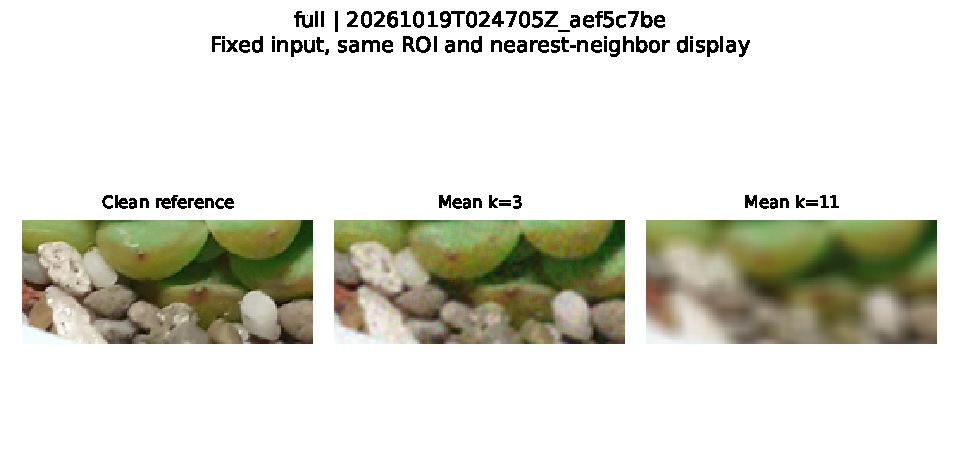
\includegraphics[width=0.80\textwidth,trim=0 35pt 0 65pt,clip]{../results/part_a/official/20261019T024705Z_aef5c7be/figures/gaussian_kernel_comparison_gravel.pdf}
\caption{Mean $3\times3$ versus $11\times11$ in the gravel region at Gaussian $\sigma_n=20$, seed 42. The broader kernel merges fine structures and softens nearby boundaries; the notebook compares all five kernel sizes.}
\label{fig:a-kernel}
\end{figure}

\textbf{Sharpening and failure cases.}\par
Sharpening does not consistently improve reference fidelity. At Gaussian $\sigma_n=20$, the illustrative Laplacian $k=3$, $\alpha=0.1$ after the selected Gaussian denoiser changes PSNR from 31.2319 to 31.2305 dB and reduces SSIM from 0.82511 to 0.81441. The selected $k=7$, $\alpha=0.1$ chain performs better, showing that aperture and strength must be assessed together.
\begin{figure}[H]
\centering
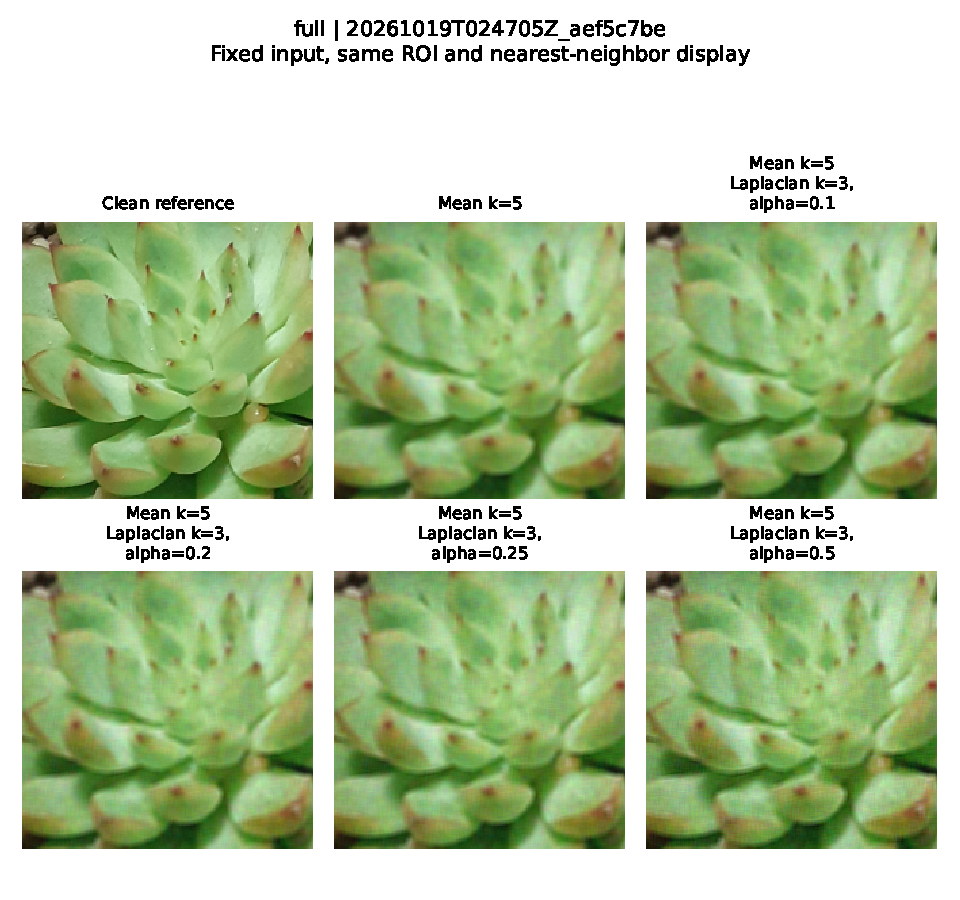
\includegraphics[width=0.64\textwidth,trim=0 80pt 0 75pt,clip]{../results/part_a/official/20261019T024705Z_aef5c7be/figures/gaussian_sharpening_comparison_leaf_edges.pdf}
\caption{Mean $5\times5$ followed by Laplacian $k=3$ with increasing $\alpha$, at Gaussian $\sigma_n=20$, seed 42. Stronger sharpening increases residual variation and local edge contrast.}
\label{fig:a-sharpening}
\end{figure}

Stronger enhancement makes leaf boundaries harsher and amplifies residual variation. Light/dark overshoot is a halo risk, but these crops do not establish repeated oscillatory ringing. Increased boundary contrast should therefore be compared with the reference rather than automatically interpreted as recovered detail.
\begin{figure}[H]
\centering
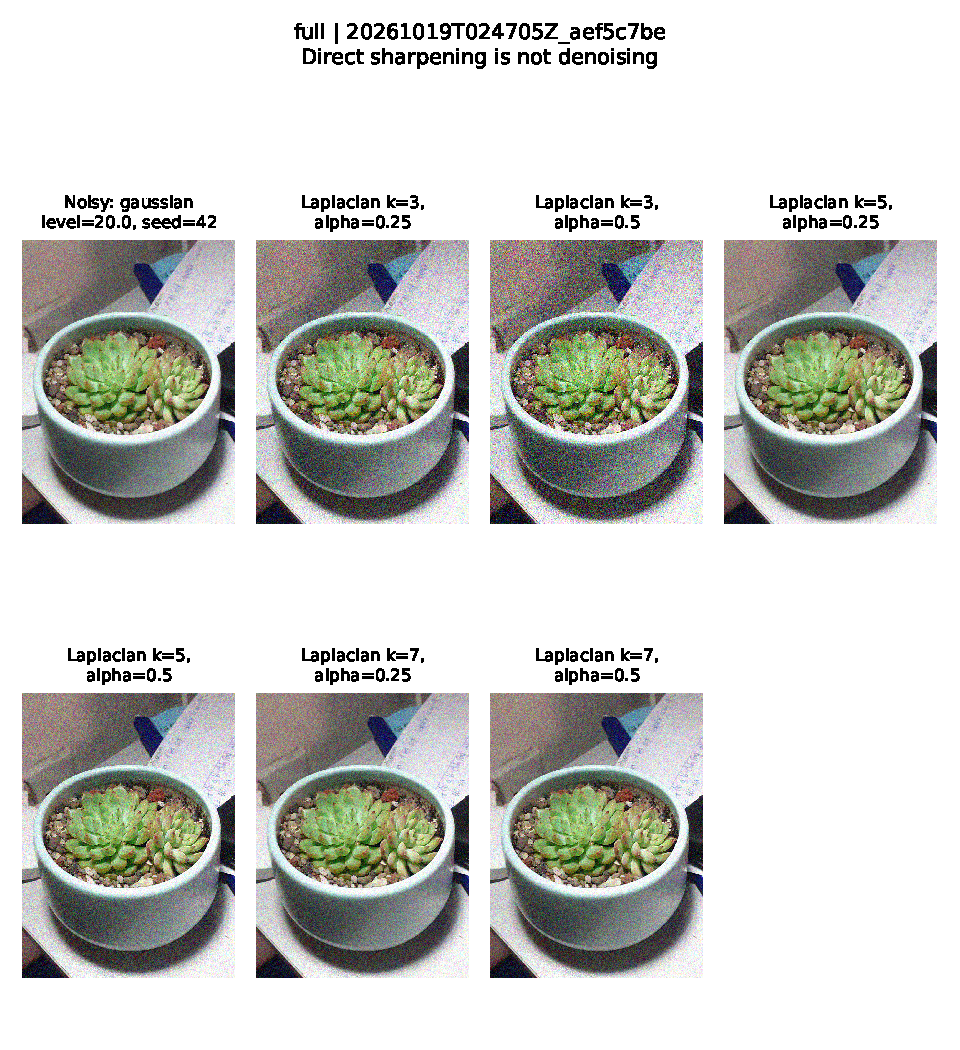
\includegraphics[width=0.94\textwidth,height=0.44\textheight,trim=0 25pt 0 75pt,clip,keepaspectratio]{../results/part_a/official/20261019T024705Z_aef5c7be/figures/gaussian_sharpening_direct.pdf}
\caption{Direct Laplacian sharpening of Gaussian-corrupted input at $\sigma_n=20$, seed 42. Panels read left to right, top to bottom; labels identify the measured settings.}
\label{fig:a-direct}
\end{figure}

Applying Laplacian $k=3$, $\alpha=0.5$ directly to the noisy image reduces whole-image PSNR from 22.3294 to 16.4111 dB and SSIM from 0.28528 to 0.13111. This failure supports denoising before enhancement. The accompanying results include direct-sharpening measurements for both noise types, all three apertures, and both tested strengths.

\textbf{Scope and limitations.}\par
Parameters are selected and evaluated using the same reference image and three seeds. The choices describe the best measured configurations for this image and objective; they do not establish performance on unseen photographs. In the broader search, Gaussian $9\times9$, $\sigma_f=1.5$ and $7\times7$, $\sigma_f=1.6$ differ by only about 0.0023 dB at $\sigma_n=30$, so the selected aperture does not imply a substantial perceptual advantage. Resizing and the large smooth background influence the measured trade-offs. Runtime belongs to the recorded environment and includes validation and conversion overhead. Additional images and independent evaluation seeds would help assess generalization.

\clearpage
\section{Part B: 3D Reconstruction}
\label{sec:part-b}
\subsection{Methodology}

\subsubsection{Input pair and processing workflow}
The experiment uses the Venus sequence from the Middlebury Optical Flow dataset. The left/reference image is \texttt{frame10.png}; the right/target image is \texttt{frame11.png}. Both are RGB images of size $420\times380$. They are exact crops of the corresponding rectified Venus stereo views: the left crop starts at $(10,0)$ and the right crop at $(0,0)$ in the $434\times383$ source images. No additional resizing or warping is applied. The accompanying \texttt{flow10.flo} field has zero vertical displacement over all $159{,}600$ pixels. For this verified horizontally rectified pair, its horizontal component gives disparity ground truth as $d_{\mathrm{GT}}=-u$, where $u$ is horizontal optical flow. This conversion is specific to the documented pair; an optical-flow file does not generally represent stereo disparity.\footnote{Middlebury, \emph{Optical Flow: Other Datasets}, \url{https://vision.middlebury.edu/flow/data/}. The source stereo views and crop coordinates were checked against the Venus archive at \url{https://vision.middlebury.edu/stereo/data/scenes2001/data/venus/venus.zip}.}

\begin{center}
\small
\fbox{Rectified Venus pair and flow-derived disparity}\\[3pt]
$\downarrow$\\[3pt]
\fbox{SIFT correspondences and RANSAC fundamental matrix}\\[3pt]
$\downarrow$\\[3pt]
\fbox{BM and SGBM parameter comparisons}\\[3pt]
$\downarrow$\\[3pt]
\fbox{Left--right consistency, GT metrics, and assumed-model reprojection}
\end{center}

\subsubsection{Sparse geometry}
SIFT detects up to 5,000 features in each image. Brute-force L2 matching retrieves the two nearest neighbours for each query descriptor; a match is retained when $d_1<0.75d_2$. The resulting correspondences estimate a $3\times3$ fundamental matrix $F$ with USAC\_MAGSAC, confidence $0.999$, at most 5,000 iterations, and pixel thresholds of $0.5$, $1$, and $2$. The native USAC random state is zero; the project seed is 42. Ground-truth flow is used only for independent diagnostics and disparity evaluation, not to estimate $F$.\footnote{OpenCV, \emph{USAC: Universal RANSAC}, \url{https://docs.opencv.org/4.x/de/d3e/tutorial_usac.html}; OpenCV, \emph{Camera Calibration and 3D Reconstruction}, \url{https://docs.opencv.org/4.x/d9/d0c/group__calib3d.html}.}

For homogeneous image points $\mathbf{x}_L$ and $\mathbf{x}_R$, corresponding points satisfy
\begin{equation}
\mathbf{x}_R^{\mathsf T}F\mathbf{x}_L=0,\qquad
\boldsymbol{\ell}_R=F\mathbf{x}_L,\quad
\boldsymbol{\ell}_L=F^{\mathsf T}\mathbf{x}_R.
\end{equation}
The reported symmetric point-to-line error is the mean of the distances in the two images,
\begin{equation}
e_{\mathrm{epi}}=\frac{|\mathbf{x}_R^{\mathsf T}F\mathbf{x}_L|}{2}
\left(\frac{1}{\sqrt{\ell_{R,1}^2+\ell_{R,2}^2}}+
\frac{1}{\sqrt{\ell_{L,1}^2+\ell_{L,2}^2}}\right).
\end{equation}
The Sampson distance is also computed as a first-order geometric approximation. Epipolar lines are drawn in both views for visual inspection. The estimated matrices and inlier masks are retained with the experiment outputs.

\subsubsection{Dense disparity and 3D reprojection}
Block Matching (BM) and Semi-Global Block Matching (SGBM) are evaluated with $\texttt{numDisparities}\in\{32,64\}$, $\texttt{blockSize}\in\{5,9,15\}$, and $\texttt{minDisparity}=-16$. BM uses an XSobel prefilter; SGBM uses the three-way mode with $P_1=8b^2$ and $P_2=32b^2$, where $b$ is the block size. Both use a uniqueness ratio of 10. OpenCV returns fixed-point disparities at 1/16-pixel precision, so each map is divided by 16 before comparison or reprojection. A right-to-left match check retains pixels whose disparity disagreement is at most 1 pixel.\footnote{OpenCV stereo matching API: \url{https://docs.opencv.org/5.0/main_modules/stereo.html}. For a review of dense two-frame stereo methods, see D. Scharstein and R. Szeliski, “A Taxonomy and Evaluation of Dense Two-Frame Stereo Correspondence Algorithms,” \emph{International Journal of Computer Vision}, vol. 47, pp. 7--42, 2002, \url{https://vision.middlebury.edu/stereo/taxonomy-IJCV.pdf}.}

For a calibrated rectified pair, depth is related to disparity by
\begin{equation}
Z=\frac{fB}{d+d_{\mathrm{offs}}},\qquad
X=\frac{(x-c_{x,L})B}{d+d_{\mathrm{offs}}},\qquad
Y=\frac{(y-c_y)B}{d+d_{\mathrm{offs}}},
\label{eq:b-reprojection}
\end{equation}
where $f$ is focal length, $B$ is baseline, and $d_{\mathrm{offs}}=c_{x,R}-c_{x,L}$. No measured calibration was available. The point clouds therefore use an explicitly assumed pinhole model: a $30^\circ$ horizontal field of view on the source frame, square pixels, zero skew, parallel axes, centered source principal points, and normalized baseline $B=1$. This gives $f=434/(2\tan15^\circ)=809.855$ pixels, cropped principal points $(206.5,191)$ and $(216.5,191)$, and $d_{\mathrm{offs}}=10$ pixels. The resulting coordinates are in normalized-baseline units and do not establish physical depth accuracy. The field-of-view choice follows Basha et al.; the remaining camera parameters are project assumptions.\footnote{T. Basha, Y. Moses, and N. Kiryati, “Multi-view Scene Flow Estimation: A View Centered Variational Approach,” \emph{International Journal of Computer Vision}, vol. 101, pp. 6--21, 2013, Sec. 4.1, \url{https://doi.org/10.1007/s11263-012-0542-7}.}

\subsection{Implementation and Results}

\subsubsection{Dataset, environment, and evaluation}
The input files, source metadata, and result artifacts are recorded in the completed run \texttt{20261019T103316Z\_9fe8bb55}. The evaluation domain contains $157{,}906$ GT-valid pixels whose flow target remains inside the right image; valid-disparity ratios use all $159{,}600$ image pixels. RMSE and bad-pixel rate are conditional on the intersection of the GT domain and the left--right-consistent prediction mask. A bad pixel has absolute disparity error greater than 1 pixel. No occlusion ground-truth mask is available, so left--right consistency is a reliability estimate rather than an occlusion label.

For prediction $d$ and ground truth $d_{\mathrm{GT}}$, the reported quantities are
\begin{equation}
\mathrm{ValidRatio}=100\frac{N_{\mathrm{LR}}}{WH},\quad
\mathrm{RMSE}=\sqrt{\frac{1}{N}\sum_{i\in\mathcal{E}}(d_i-d_{\mathrm{GT},i})^2},\quad
\mathrm{BadRate}=100\frac{N_{\mathrm{bad}}}{N},
\end{equation}
where $\mathcal{E}$ is the prediction-valid intersection with the GT evaluation domain, $N=|\mathcal{E}|$, and $N_{\mathrm{bad}}$ counts errors greater than 1 pixel. Coverage in Table~\ref{tab:b-dense} is $100N/157{,}906$; it is distinct from the all-image valid ratio. Each dense configuration has three warm-ups and 20 timed repetitions. OpenCV 5.0.0 ran with one thread and OpenCL disabled; the environment used Python 3.13.14 and NumPy 2.5.4. The reported median time includes matcher construction, both matching directions, disparity conversion, and consistency checking; it excludes file I/O, metric computation, figures, and 3D reprojection.

\begin{figure}[htbp]
\centering
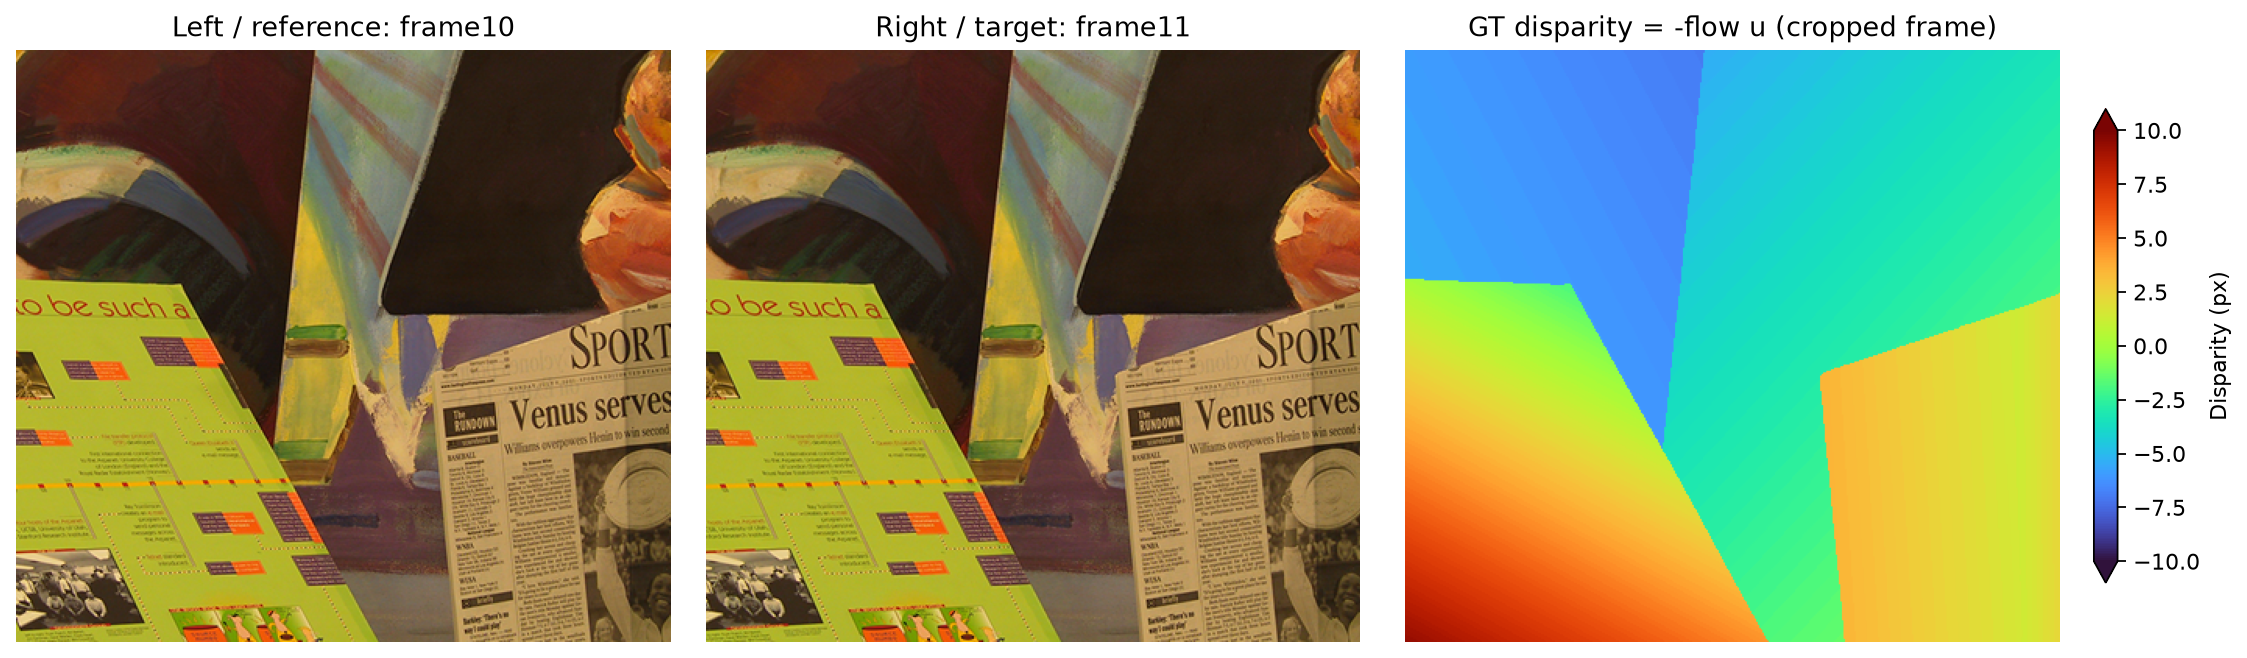
\includegraphics[width=0.98\textwidth]{../results/part_b/20261019T103316Z_9fe8bb55/figures/input_and_ground_truth.png}
\caption{Venus stereo pair and flow-derived disparity. The disparity display is clipped to $[-10,10]$ pixels for visualization; the original flow values are used for evaluation.}
\label{fig:b-input}
\end{figure}

\subsubsection{Fundamental matrix and epipolar geometry}
The detector returned 629 left and 567 right keypoints. KNN produced 629 candidate pairs; 411 passed the ratio test. Table~\ref{tab:b-geometry} reports all three RANSAC thresholds. As the threshold increases, more matches are retained as inliers, while the mean error among those inliers also increases. Independent GT-domain checks yield mean symmetric epipolar errors close to 0.11 pixels. The 95th-percentile absolute epipolar-line angle is below $2^\circ$ in both views for every estimate, a project diagnostic for this rectified pair rather than a grading threshold.

\begin{table}[htbp]
\centering
\footnotesize
\setlength{\tabcolsep}{4pt}
\caption{Sparse geometry results. Each estimate uses the same 411 ratio-test matches. GT-domain error is evaluated independently on the 157,906 flow-derived correspondences.}
\label{tab:b-geometry}
\begin{tabular}{rrrrr}
\toprule
\multicolumn{1}{c}{Threshold (px)} & \multicolumn{1}{c}{Inliers} & \multicolumn{1}{c}{Inlier ratio (\%)} & \multicolumn{1}{c}{Inlier epi. mean (px)} & \multicolumn{1}{c}{GT-domain epi. mean (px)} \\
\midrule
0.5 & 378 & 91.97 & 0.0921 & 0.1150 \\
1.0 & 385 & 93.67 & 0.1049 & 0.1124 \\
2.0 & 392 & 95.38 & 0.1392 & 0.1150 \\
\bottomrule
\end{tabular}
\end{table}

Feature detection and matching took 120.743 ms in a single measurement; the three RANSAC fits took 8.828, 3.704, and 3.083 ms at thresholds 0.5, 1, and 2 pixels, respectively. These sparse-stage timings are single samples and are separate from the repeated dense-matching measurements.

\begin{figure}[htbp]
\centering
\begin{subfigure}{0.48\textwidth}
  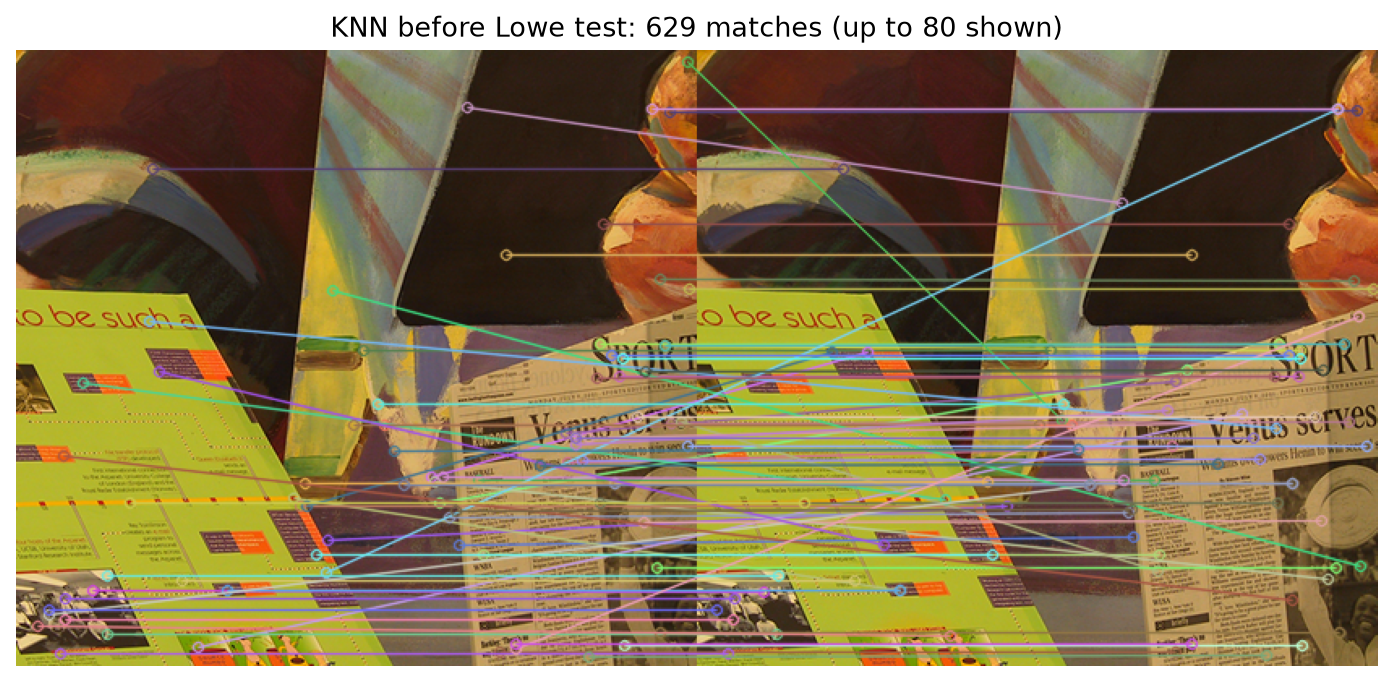
\includegraphics[width=\linewidth]{../results/part_b/20261019T103316Z_9fe8bb55/figures/initial_matches.png}
  \caption{Initial descriptor matches.}
\end{subfigure}\hfill
\begin{subfigure}{0.48\textwidth}
  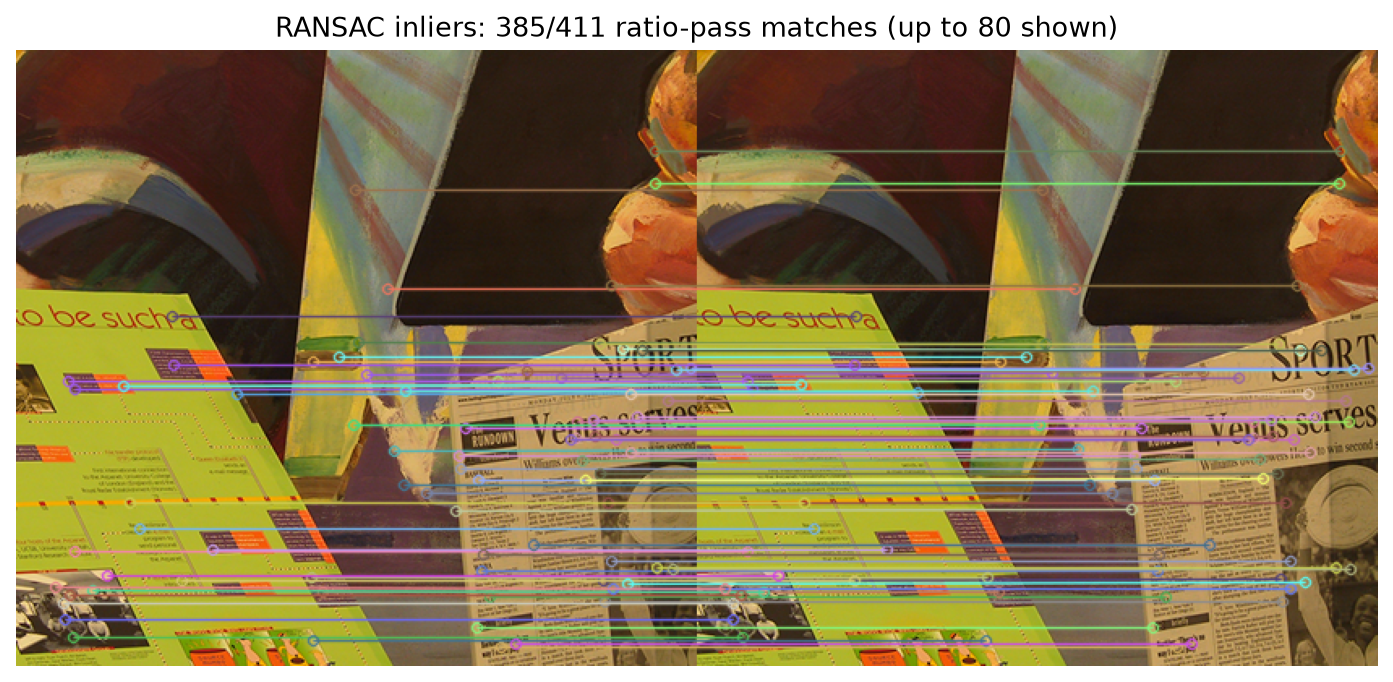
\includegraphics[width=\linewidth]{../results/part_b/20261019T103316Z_9fe8bb55/figures/inlier_matches.png}
  \caption{RANSAC inliers.}
\end{subfigure}
\caption{SIFT correspondences before and after robust fundamental-matrix estimation.}
\label{fig:b-matches}
\end{figure}

\begin{figure}[htbp]
\centering
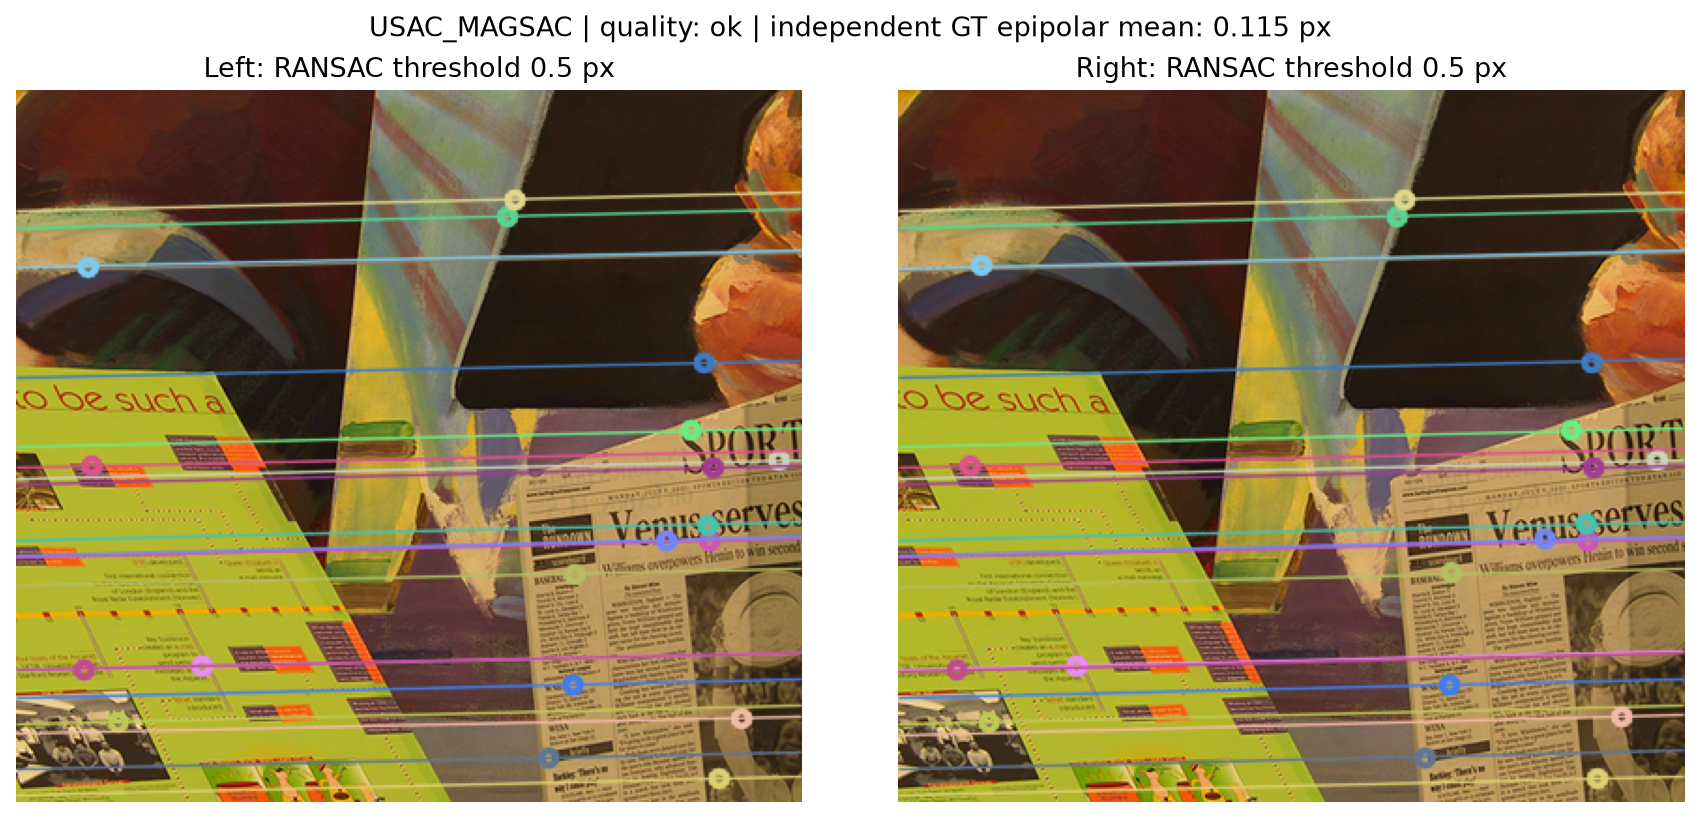
\includegraphics[width=0.98\textwidth]{../results/part_b/20261019T103316Z_9fe8bb55/figures/ransac_t0p5_epipolar.png}
\caption{Epipolar lines generated by the $0.5$-pixel USAC\_MAGSAC estimate, shown in both images. Its independent GT-domain mean symmetric epipolar error is 0.115 pixels.}
\label{fig:b-epipolar}
\end{figure}

\subsubsection{Dense matching results}
Table~\ref{tab:b-dense} summarizes all 12 configurations. SGBM provides greater valid coverage and lower conditional error than BM for each tested parameter pair, at a higher measured runtime. Figure~\ref{fig:b-bm} and Figure~\ref{fig:b-sgbm} show the left--right-consistent maps. Gray regions are invalid; the color display saturates outside $[-10,10]$ pixels, while the saved floating-point disparities remain unchanged.

\begin{table}[htbp]
\centering
\footnotesize
\setlength{\tabcolsep}{3pt}
\caption{Dense disparity comparison. LR-valid ratio is over all image pixels; coverage, RMSE, and bad-pixel rate use the GT-domain intersection with LR-consistent predictions. Runtime is the median of 20 repetitions in milliseconds.}
\label{tab:b-dense}
\begin{tabular}{lrrrrr}
\toprule
\shortstack{Method / $n_{\mathrm{disp}}$\\block} & \multicolumn{1}{c}{LR-valid ratio (\%)} & \multicolumn{1}{c}{Coverage (\%)} & \multicolumn{1}{c}{RMSE (px)} & \multicolumn{1}{c}{Bad $>1$ px (\%)} & \multicolumn{1}{c}{Median (ms)} \\
\midrule
BM / 32 / 5  & 68.483 & 69.218 & 1.7335 & 5.101 & 15.942 \\
BM / 32 / 9  & 78.730 & 79.575 & 0.8964 & 2.929 & 16.663 \\
BM / 32 / 15 & 82.562 & 83.448 & 0.8116 & 3.322 & 32.676 \\
BM / 64 / 5  & 53.749 & 54.325 & 3.6564 & 5.682 & 36.027 \\
BM / 64 / 9  & 64.126 & 64.814 & 1.0868 & 3.280 & 18.381 \\
BM / 64 / 15 & 68.690 & 69.427 & 0.8509 & 3.733 & 18.003 \\
SGBM / 32 / 5  & 90.510 & 91.481 & 0.5341 & 1.521 & 27.308 \\
SGBM / 32 / 9  & 90.532 & 91.503 & 0.6109 & 2.011 & 27.725 \\
SGBM / 32 / 15 & 90.538 & 91.510 & 0.7162 & 2.851 & 49.016 \\
SGBM / 64 / 5  & 76.409 & 77.228 & 0.5538 & 1.697 & 67.800 \\
SGBM / 64 / 9  & 76.415 & 77.235 & 0.6341 & 2.266 & 61.293 \\
SGBM / 64 / 15 & 76.445 & 77.266 & 0.7458 & 3.236 & 68.425 \\
\bottomrule
\end{tabular}
\end{table}

\begin{figure}[htbp]
\centering
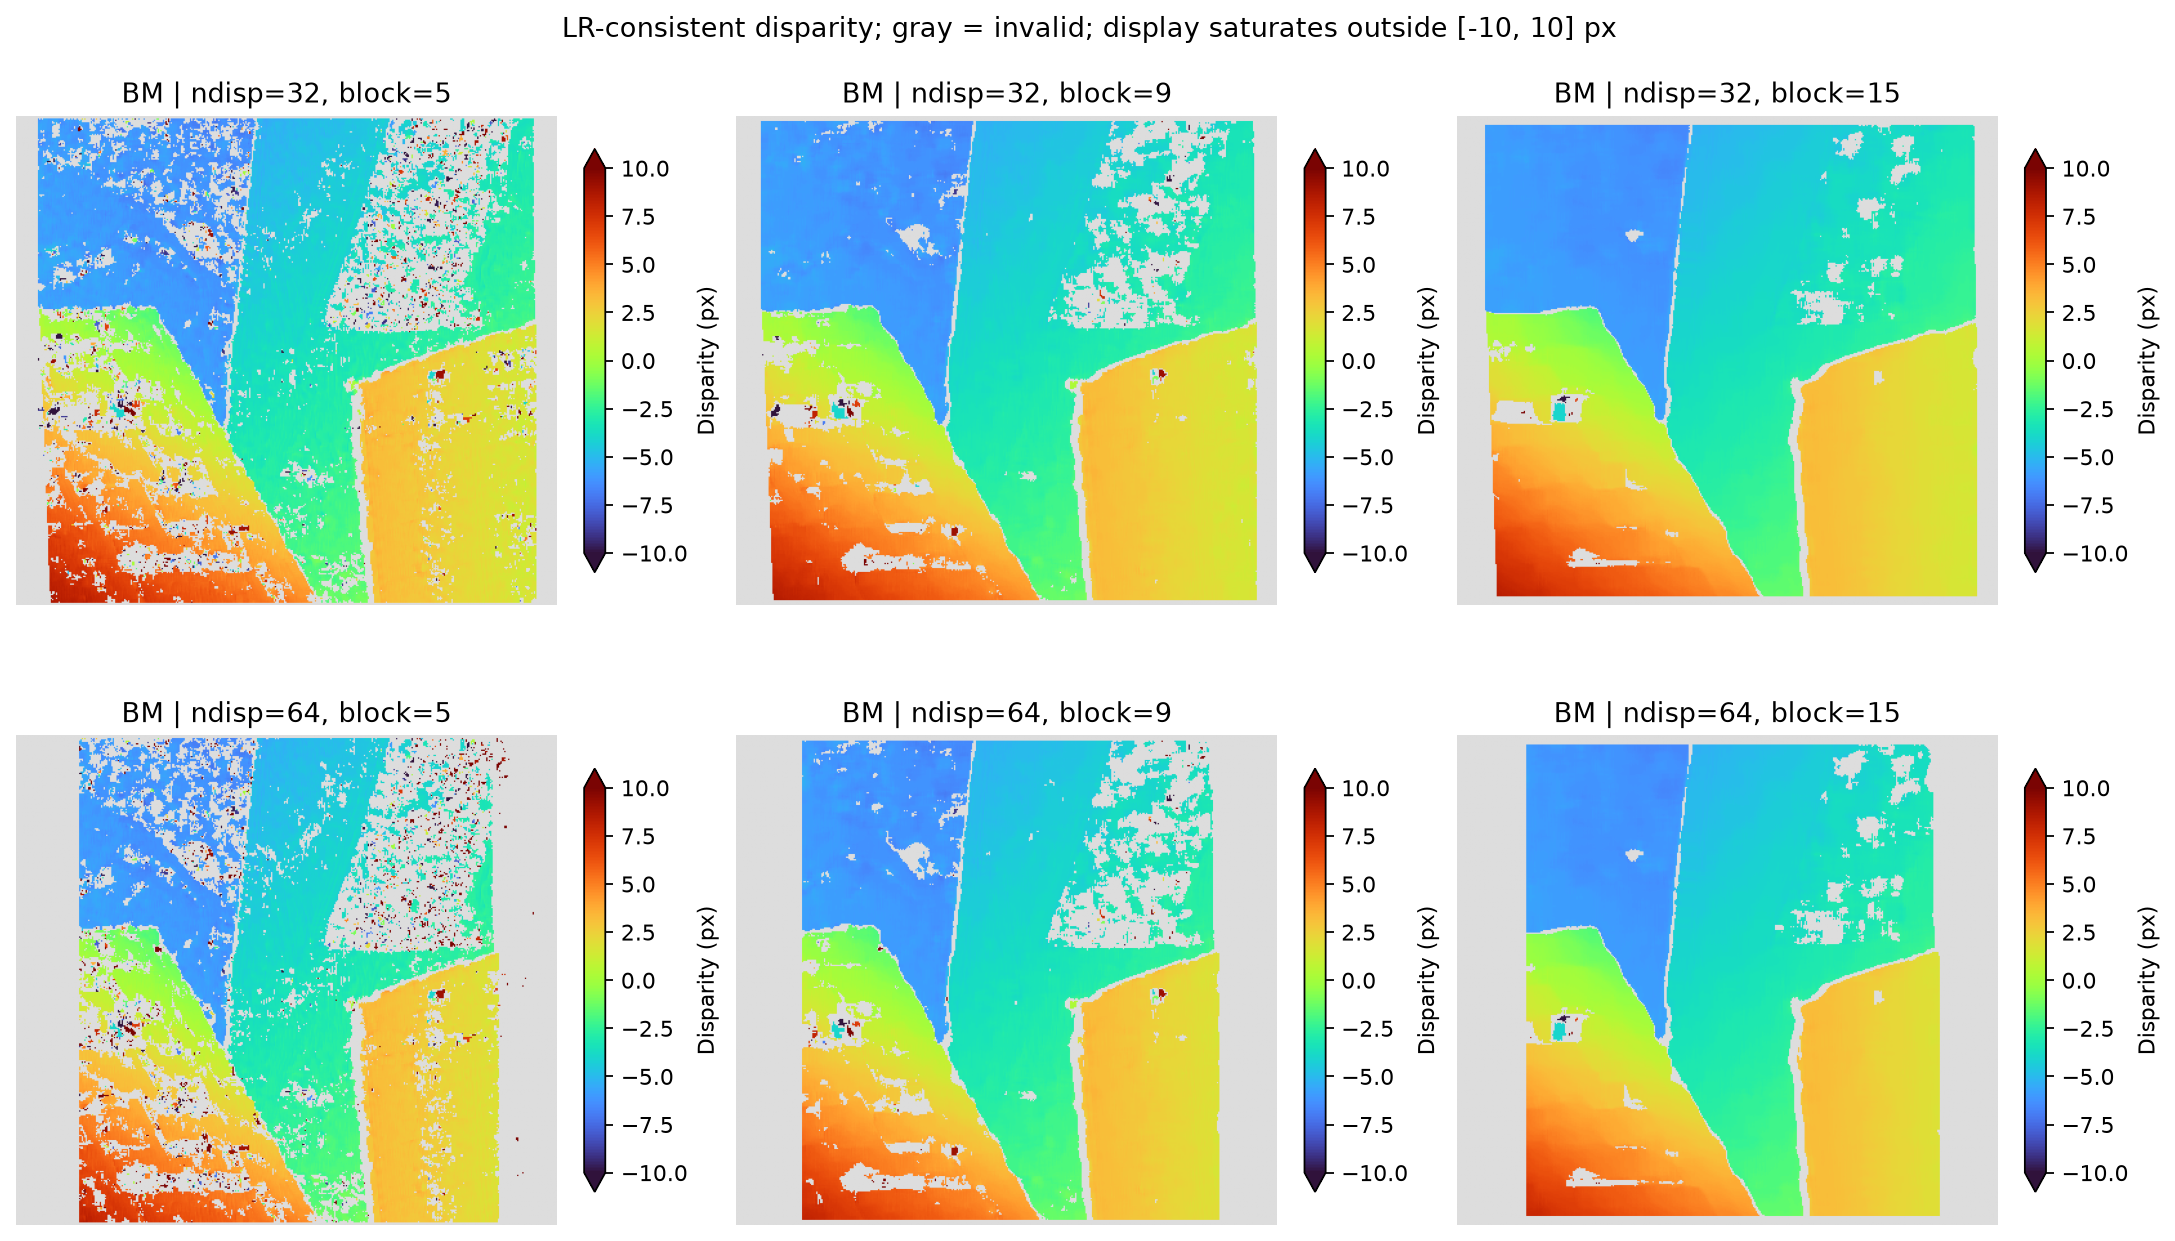
\includegraphics[width=0.98\textwidth]{../results/part_b/20261019T103316Z_9fe8bb55/figures/bm_disparity_grid.png}
\caption{BM left--right-consistent disparity maps for the six tested combinations of disparity range and block size.}
\label{fig:b-bm}
\end{figure}

\begin{figure}[htbp]
\centering
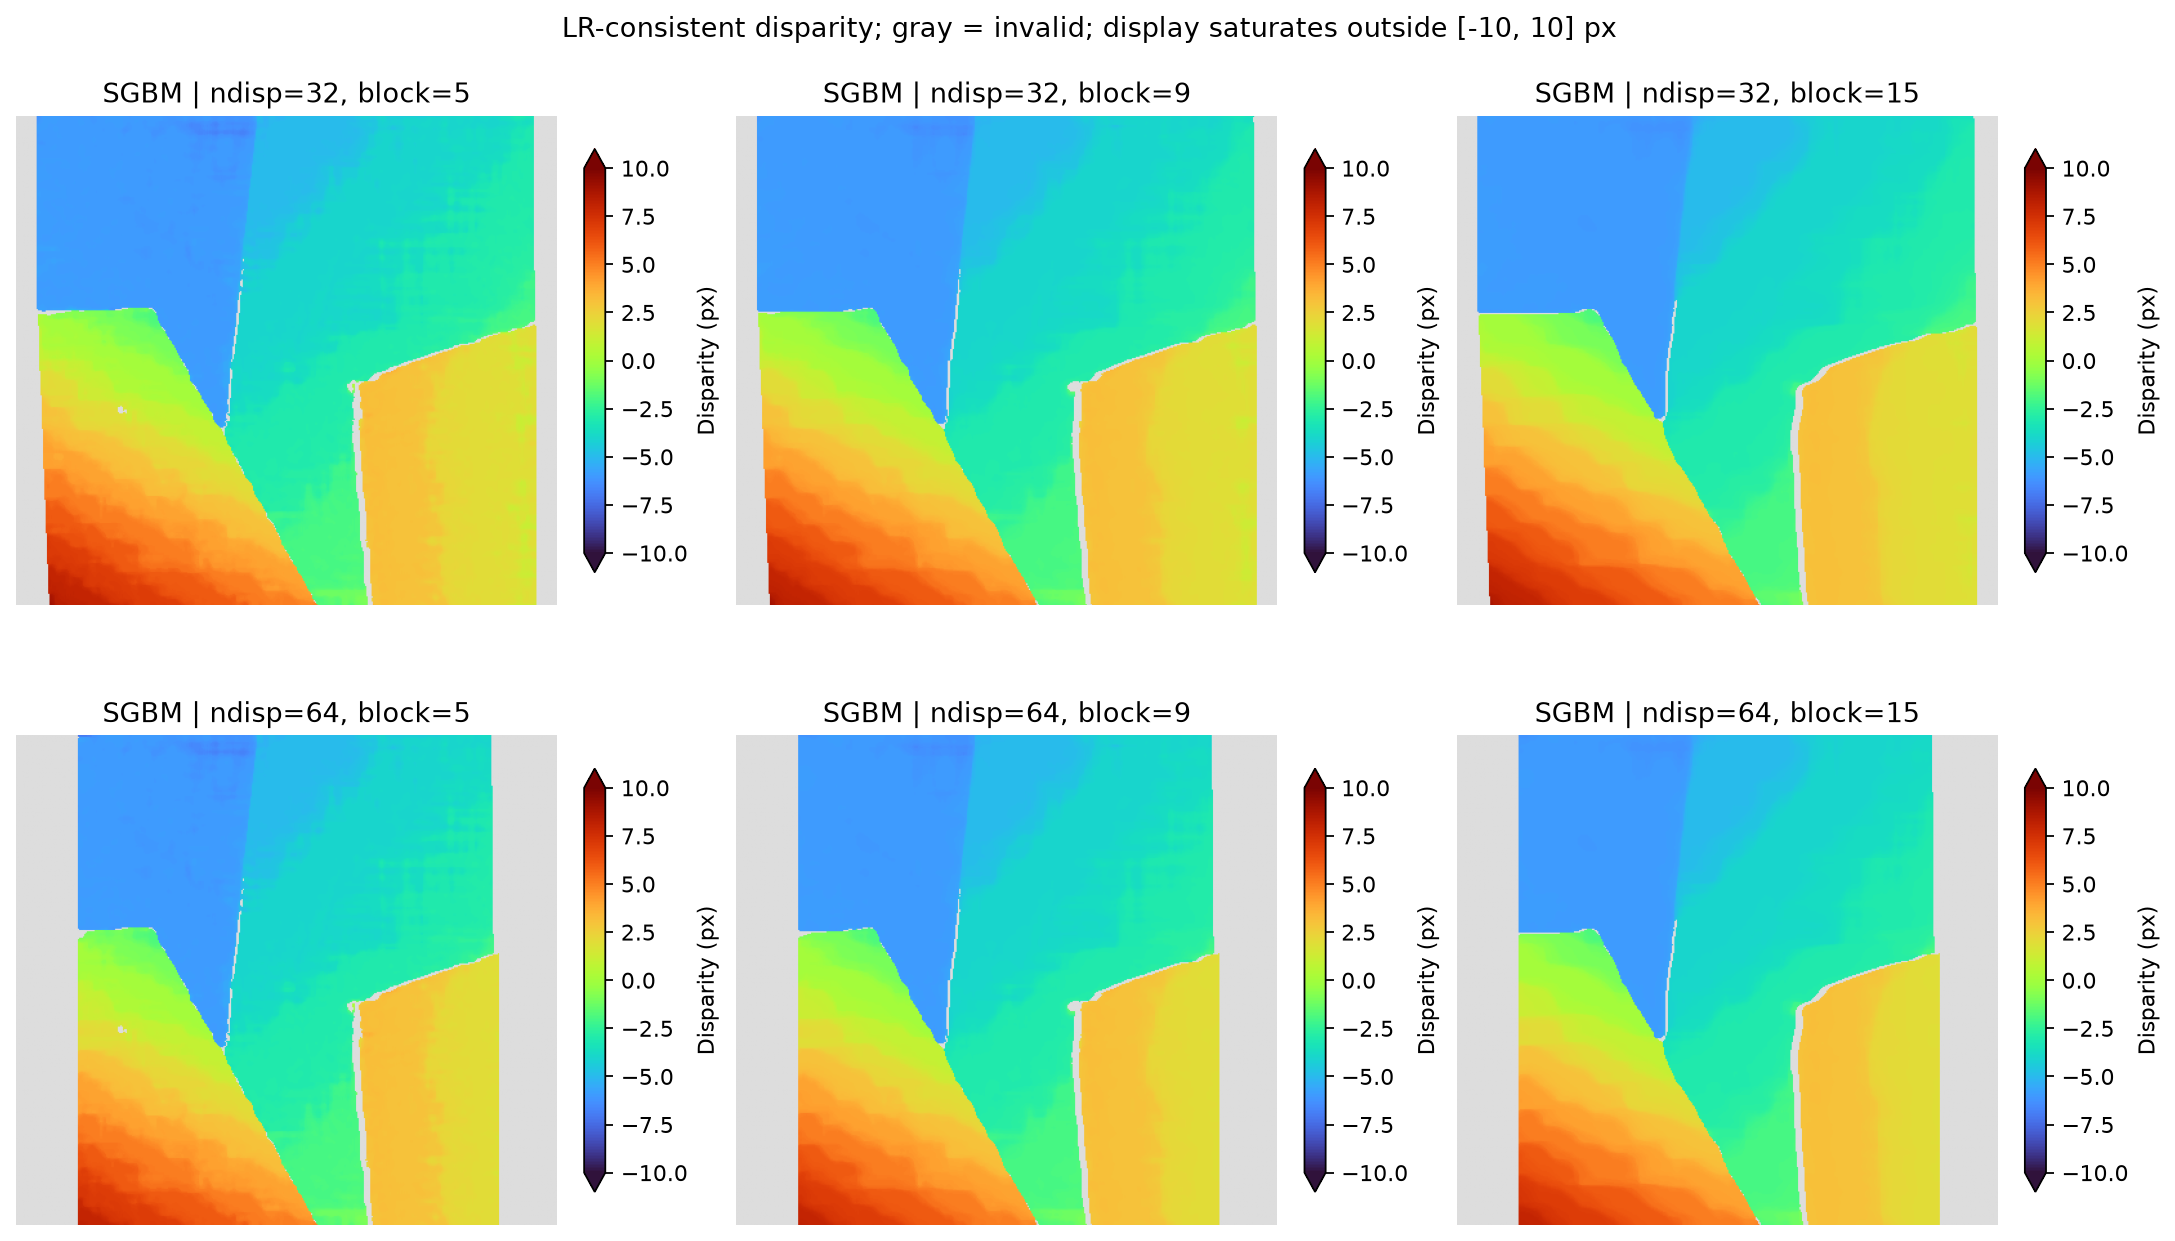
\includegraphics[width=0.98\textwidth]{../results/part_b/20261019T103316Z_9fe8bb55/figures/sgbm_disparity_grid.png}
\caption{SGBM left--right-consistent disparity maps for the six tested combinations of disparity range and block size.}
\label{fig:b-sgbm}
\end{figure}

\subsubsection{Point-cloud reconstruction}
For a direct point-cloud comparison, BM and SGBM use $\texttt{numDisparities}=32$ and $\texttt{blockSize}=9$. Reprojection keeps LR-consistent pixels with a positive denominator and finite positive depth. A connected-component filter removes disparity components of at most 100 pixels when adjacent disparity differences are at most 1 pixel; it does not use the GT. The BM cloud contains 125,575 raw points, of which 980 are removed, leaving 124,595. The SGBM cloud contains 144,489 points and the filter removes none. Figure~\ref{fig:b-cloud} shows the filtered SGBM cloud from three viewpoints; the full point sets are retained in the result artifacts.

\begin{figure}[htbp]
\centering
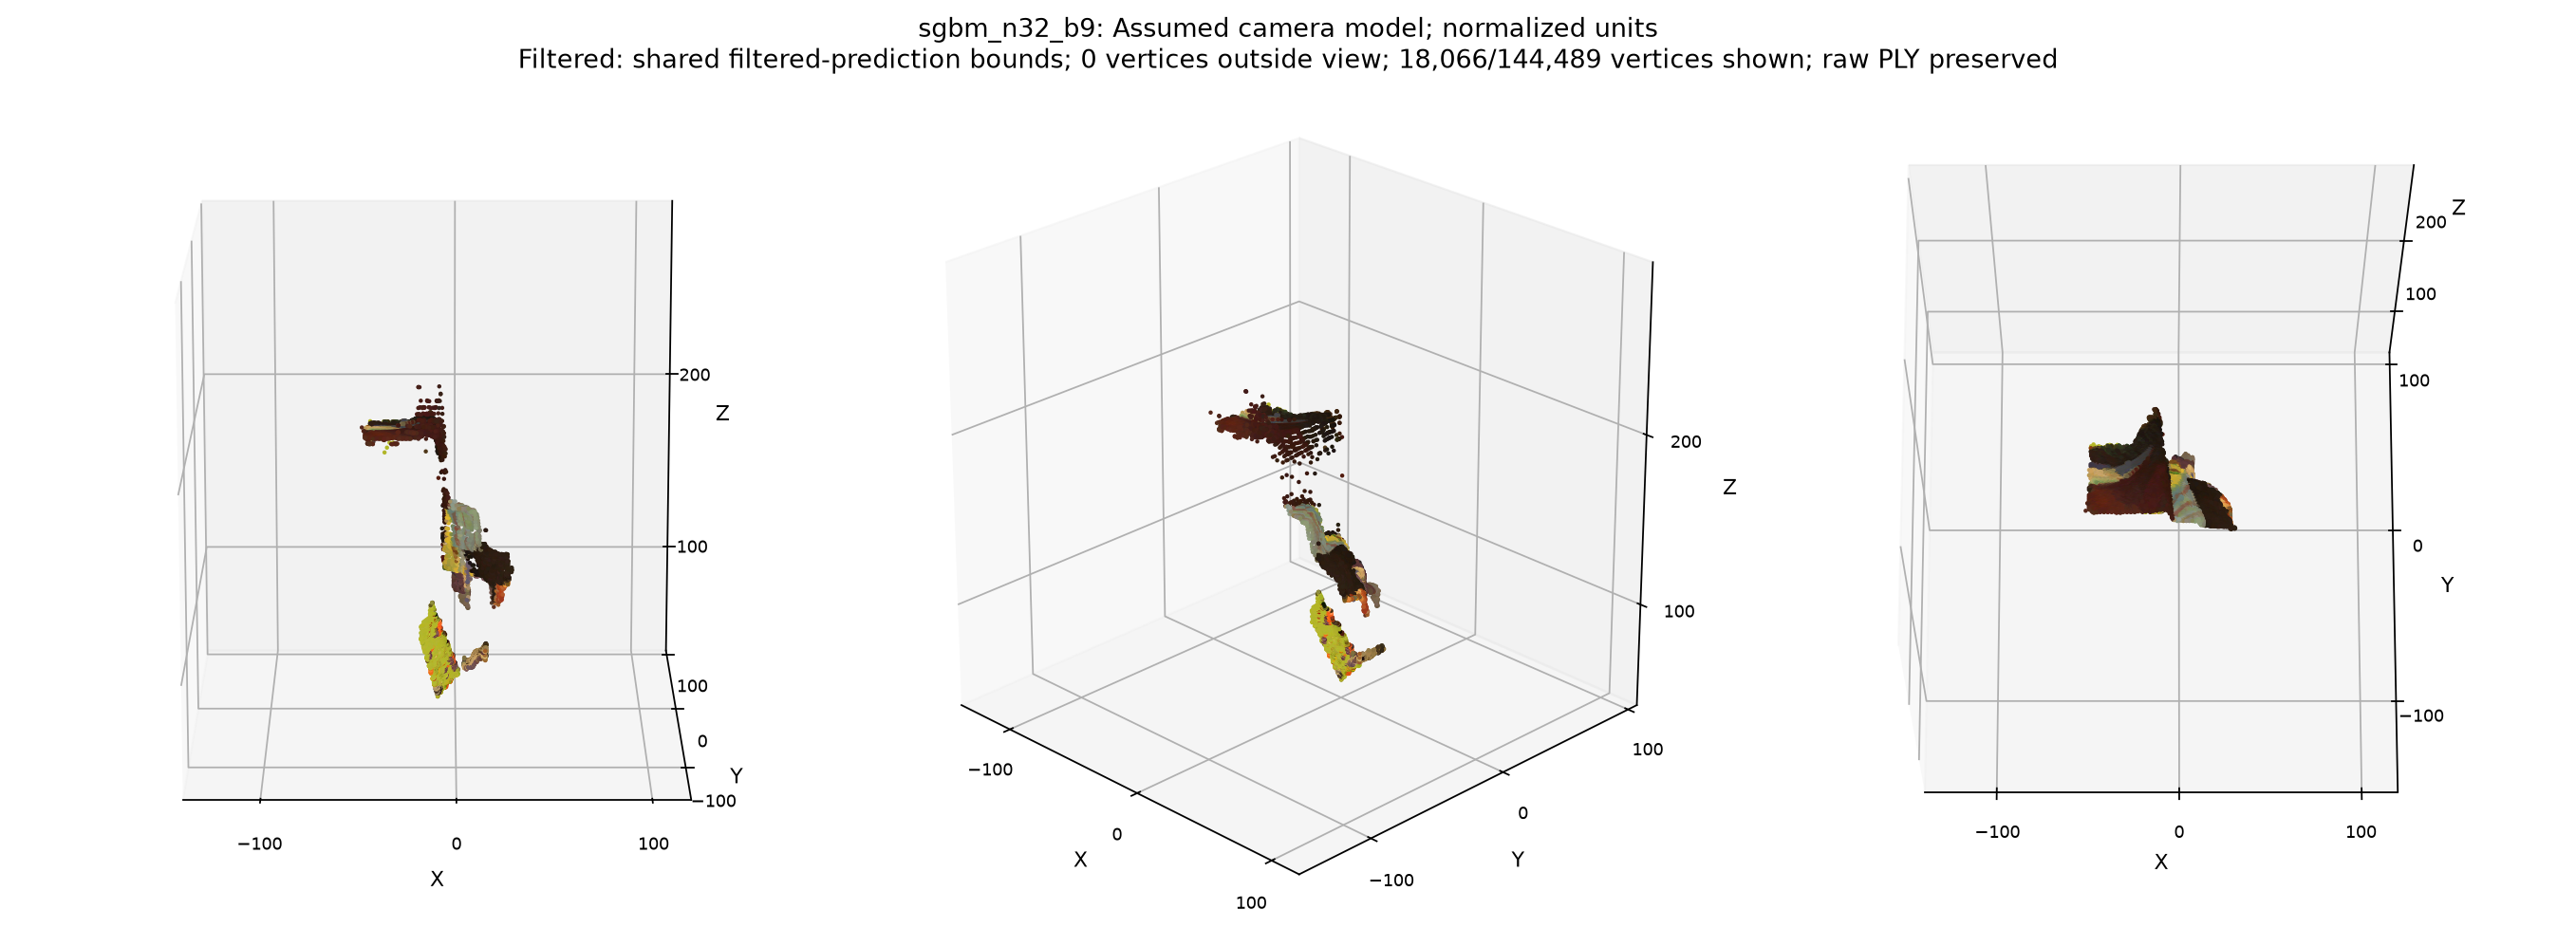
\includegraphics[width=0.98\textwidth]{../results/part_b/20261019T103316Z_9fe8bb55/figures/sgbm_n32_b9_point_cloud_filtered.png}
\caption{SGBM point cloud for $n_{\mathrm{disp}}=32$, block size 9, shown from three viewpoints. Axes are in normalized-baseline units under the assumed camera model; the plot samples points for display, while the complete cloud is preserved.}
\label{fig:b-cloud}
\end{figure}

\subsection{Comparative Analysis}

\subsubsection{Accuracy, coverage, and runtime}
SGBM's advantage is consistent across the tested grid: its best RMSE is 0.5341 pixels at $n_{\mathrm{disp}}=32$, block size 5, compared with the best BM RMSE of 0.8116 pixels at $n_{\mathrm{disp}}=32$, block size 15. SGBM also has the lower bad-pixel rate in each paired setting. At $n_{\mathrm{disp}}=32$, its LR-valid ratio is about 90.5\%, compared with 68.5--82.6\% for BM. The difference remains when both methods are evaluated on exactly the same pixels at block size 9: RMSE is 0.5959 pixels for SGBM and 0.8792 pixels for BM; bad-pixel rates are 1.93\% and 2.74\%, respectively, over the common 125,276-pixel domain. Thus the lower SGBM error is not explained solely by its larger valid region.

This accuracy and coverage come with greater cost in this run. The fastest SGBM case takes 27.308 ms, while the fastest BM case takes 15.942 ms under the same timing protocol. Increasing the disparity range to 64 reduces coverage in both methods for this pair and gives no better RMSE than the best 32-disparity setting. Within SGBM, larger blocks slightly increase coverage but also raise RMSE and bad-pixel rate. BM block size 15 gives the lowest RMSE among BM cases, but its bad-pixel rate is higher than BM at block size 9. These measurements support a trade-off rather than one parameter setting that optimizes every metric.

\subsubsection{Visual quality and limitations}
The disparity grids show BM's block- and range-dependent invalid areas and speckled responses, especially with a 5-pixel block. Larger BM blocks produce more continuous regions but smooth local variation. SGBM maps are more spatially regular and preserve higher valid coverage, although boundaries are softened and invalid strips remain near some occlusions and image borders. These observations describe the displayed Venus pair; no occlusion ground truth is available to classify every invalid or mismatched pixel.

With assumed focal length, principal points, crop offset, and $B=1$, these clouds show qualitative normalized depth. Measured camera calibration remains unavailable, so calibrated 3D reconstruction and physical depth accuracy remain unverified. The point-cloud demonstration does not establish completion of the calibrated-reconstruction requirement. Runtimes apply only to this recorded environment.

\clearpage

\section{Part C: Image Stitching}
\label{sec:part-c}

\subsection{Methodology}

\subsubsection{Image sequence and coordinate frame}
The experiment uses four ordered, overlapping 1920$\times$1080 PNG images of the interior of Chua Minh Thanh, photographed by the student during a trip to Gia Lai. The input files are \texttt{pagoda\_01.png} through \texttt{pagoda\_04.png}; image 3 defines the common coordinate frame. Images 1, 2, and 4 are each mapped directly to image 3, while image 3 uses the identity transform. The inputs are not resized, cropped, or rectified. The run snapshot preserves the source images and their SHA-256 checksums. Figure~\ref{fig:c-pipeline} summarizes the stitching and evaluation stages.

\begin{figure}[htbp]
\centering
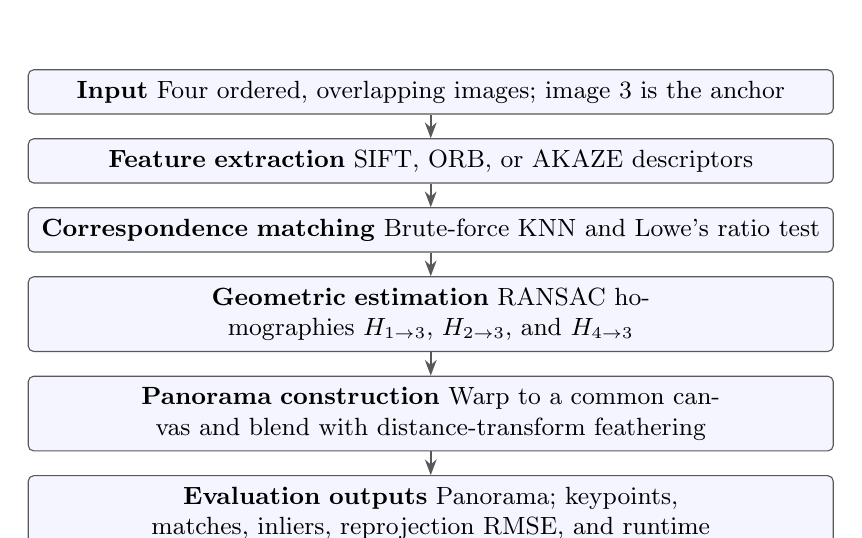
\begin{tikzpicture}[
  process/.style={draw=black!65, rounded corners=2pt, fill=blue!4,
    text width=0.82\textwidth, align=center, inner sep=4pt, font=\small},
  flow/.style={-{Stealth[length=2mm]}, semithick, draw=black!65},
  node distance=3mm
]
\node[process] (input) {\textbf{Input}\ Four ordered, overlapping images; image 3 is the anchor};
\node[process, below=of input] (features) {\textbf{Feature extraction}\ SIFT, ORB, or AKAZE descriptors};
\node[process, below=of features] (matching) {\textbf{Correspondence matching}\ Brute-force KNN and Lowe's ratio test};
\node[process, below=of matching] (geometry) {\textbf{Geometric estimation}\ RANSAC homographies $H_{1\to3}$, $H_{2\to3}$, and $H_{4\to3}$};
\node[process, below=of geometry] (render) {\textbf{Panorama construction}\ Warp to a common canvas and blend with distance-transform feathering};
\node[process, below=of render] (evaluation) {\textbf{Evaluation outputs}\ Panorama; keypoints, matches, inliers, reprojection RMSE, and runtime};
\draw[flow] (input) -- (features);
\draw[flow] (features) -- (matching);
\draw[flow] (matching) -- (geometry);
\draw[flow] (geometry) -- (render);
\draw[flow] (render) -- (evaluation);
\end{tikzpicture}
\caption{Part C pipeline from the ordered image set to panorama construction and comparative evaluation.}
\label{fig:c-pipeline}
\end{figure}

\subsubsection{Features, matching, and homography}
The experiment compares SIFT, ORB, and AKAZE using OpenCV. SIFT uses up to 5,000 features and the L2 descriptor distance. ORB uses up to 5,000 features, \texttt{WTA\_K=2}, and Hamming distance. AKAZE uses the oriented MLDB descriptor, threshold 0.001, and a limit of 5,000 features, with Hamming distance. If a detector returns more than the limit, features are stably sorted by response and the corresponding descriptor rows are retained in the same order. Feature extraction runs on grayscale images; geometric warping uses the original colour images.

For each source image and image 3, a brute-force matcher requests the two nearest neighbours, $d_1$ and $d_2$. A match passes Lowe's ratio test when
\begin{equation}
d_1 < r d_2,
\end{equation}
where $r\in\{0.72,0.75,0.78\}$. The initial-match count is the number of KNN rows with both neighbours, before applying this test. Descriptor distance is L2 for SIFT and Hamming for ORB and AKAZE.

For each source-to-anchor pair, RANSAC estimates a homography with confidence 0.995, at most 5,000 iterations, and reprojection threshold $\tau\in\{3,4,5,6\}$ pixels:
\begin{equation}
\lambda\begin{bmatrix}u'\\v'\\1\end{bmatrix}
=H_{i\rightarrow3}\begin{bmatrix}u\\v\\1\end{bmatrix},
\qquad (u',v')=\left(\frac{q_1}{q_3},\frac{q_2}{q_3}\right),
\end{equation}
where $q=H_{i\rightarrow3}[u,v,1]^T$ and $\lambda=q_3$. The pipeline checks that point sets are non-collinear, the estimated matrix is finite and full rank, at least four inliers remain, and the projected image does not cross a projective horizon. It also checks that the common canvas is finite and contains no more than 40 million pixels. Failed configurations retain their status and reason.

\subsubsection{Warping, blending, and evaluation}
The main comparison warps all four images into the image-3 frame and uses distance-transform feather weights. Each source colour is multiplied by its weight before warping; the weighted colours and weights are accumulated separately:
\begin{equation}
P(x,y)=\frac{\sum_i \mathcal{W}_i[w_i I_i](x,y)}
{\sum_i \mathcal{W}_i[w_i](x,y)},
\end{equation}
where $\mathcal{W}_i$ warps a source array into the common canvas and $w_i$ is its source feather weight. Both the premultiplied colour $w_i I_i$ and the weight $w_i$ are warped before accumulation; division is evaluated only on valid support. The support mask comes from the weights, so black image content is not mistaken for an empty region. The output is cropped to the rectangular extent of valid support; unsupported corners within the rectangle remain masked.

Initial matches are counted before the ratio test. The inlier ratio uses all ratio-pass correspondences across the three pairs as its denominator. For pair $p$, let $n_p$ be the RANSAC inlier count and $S_p$ the sum of squared forward reprojection errors from source to image 3. The pooled measures are
\begin{equation}
\mathrm{InlierRatio}=100\frac{\sum_p n_p}{\sum_p M_p},
\qquad
\mathrm{RMSE}=\sqrt{\frac{\sum_p S_p}{\sum_p n_p}},
\end{equation}
where $M_p$ is the number of ratio-pass matches. RMSE is in pixels; pair RMSE values are not averaged directly. Keypoint totals count each of the four images once. Convex-hull coverage is reported as a spatial-support diagnostic, not as ground-truth alignment accuracy.

Each selected or baseline pipeline is measured after one warm-up and five full repetitions, with extraction and matching repeated each time. Total stitching time runs from detector creation and grayscale conversion through the cropped panorama; it excludes file I/O, metric calculation, and figure generation. The reported value is the median and IQR of five samples. OpenCV runs single-threaded with OpenCL disabled. A separate comparison holds homographies fixed and measures canvas setup, warp, blending, and crop for feathering and multi-band blending with 3, 5, and 7 bands. These stage-only timings are not added to or subtracted from the full-pipeline timings.

\subsection{Implementation and Results}

\subsubsection{Environment and parameter grid}
The pipeline uses OpenCV for feature detection, descriptor matching, homography estimation, warping, and blending. Measurements were collected with Python 3.13.14, NumPy 2.5.4, OpenCV 5.0.0 from opencv-contrib-python-headless 5.0.0.93, and Matplotlib 3.11.2 on Linux x86\_64. The accompanying reproducibility package preserves the inputs, configurations, source snapshot, homographies, masks, timings, and output checksums. The experiment tested all 12 combinations of three Lowe ratios and four RANSAC thresholds for each detector, giving 36 configurations in total. Every configuration produced a panorama, and all 108 pair records passed validation. The selected settings were reviewed visually within this image sequence and parameter grid; they are not asserted to be universal optima.

\begin{table}[htbp]
\centering
\small
\caption{Detected and retained features per image. Each detector uses at most 5,000 features; SIFT returned 5,001 on image 3 before the stable response limit.}
\label{tab:c-keypoints}
\begin{tabular}{lccc}
\toprule
Image & SIFT detected / used & ORB detected / used & AKAZE detected / used \\
\midrule
1 & 5,000 / 5,000 & 5,000 / 5,000 & 5,000 / 5,000 \\
2 & 5,000 / 5,000 & 5,000 / 5,000 & 5,000 / 5,000 \\
3 & 5,001 / 5,000 & 5,000 / 5,000 & 5,000 / 5,000 \\
4 & 5,000 / 5,000 & 5,000 / 5,000 & 5,000 / 5,000 \\
\bottomrule
\end{tabular}
\end{table}

\begin{figure}[htbp]
\centering
\begin{subfigure}[t]{0.32\textwidth}
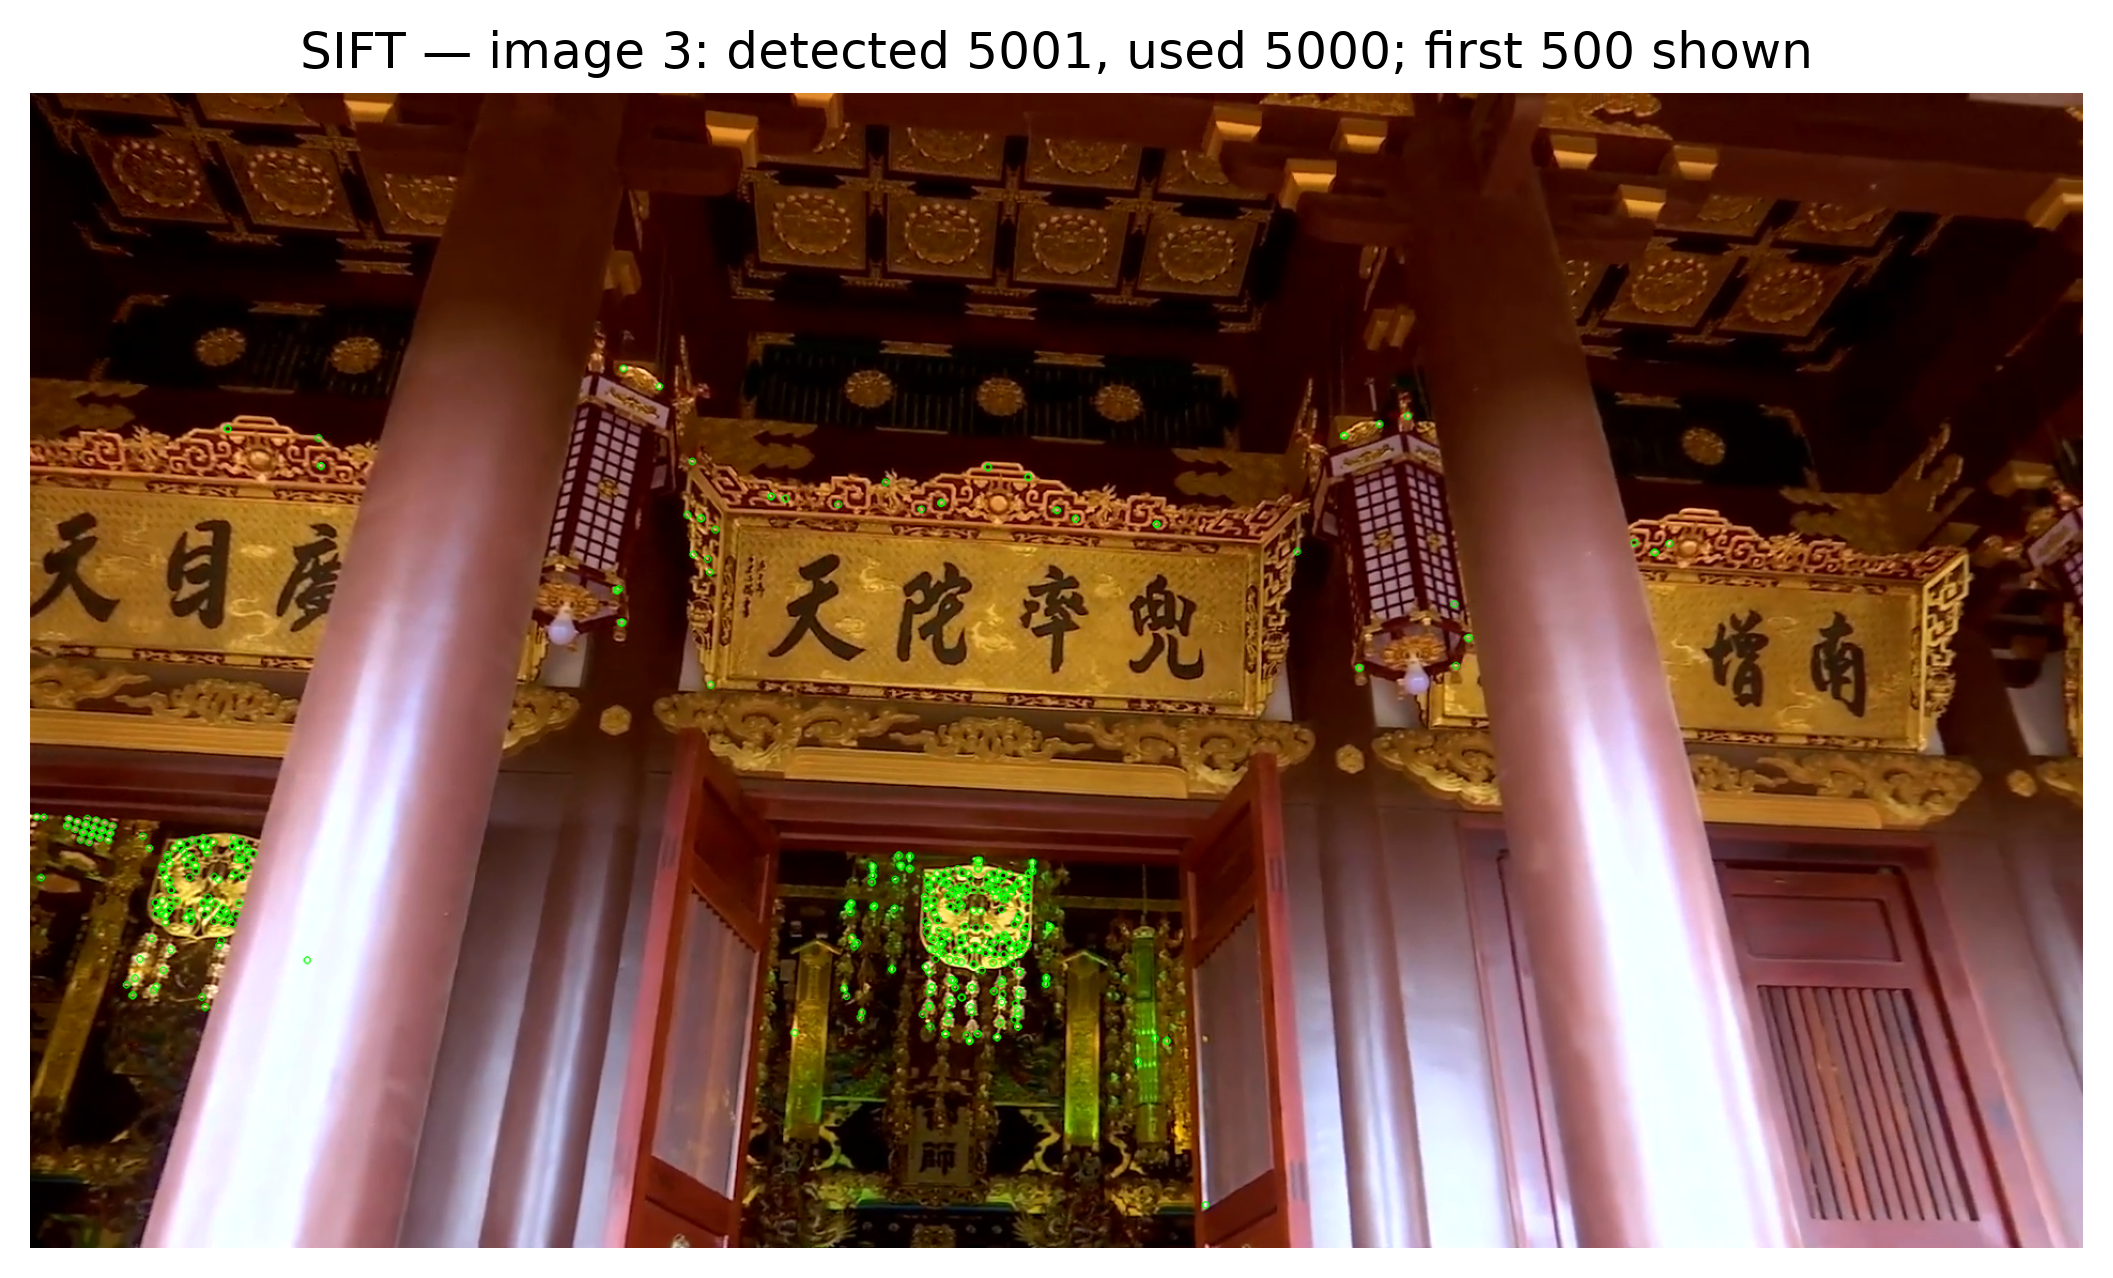
\includegraphics[width=\linewidth]{../results/part_c/refinement/20261019T105909Z_fe7aa242/figures/sift_keypoints_3.png}
\caption{SIFT}
\end{subfigure}\hfill
\begin{subfigure}[t]{0.32\textwidth}
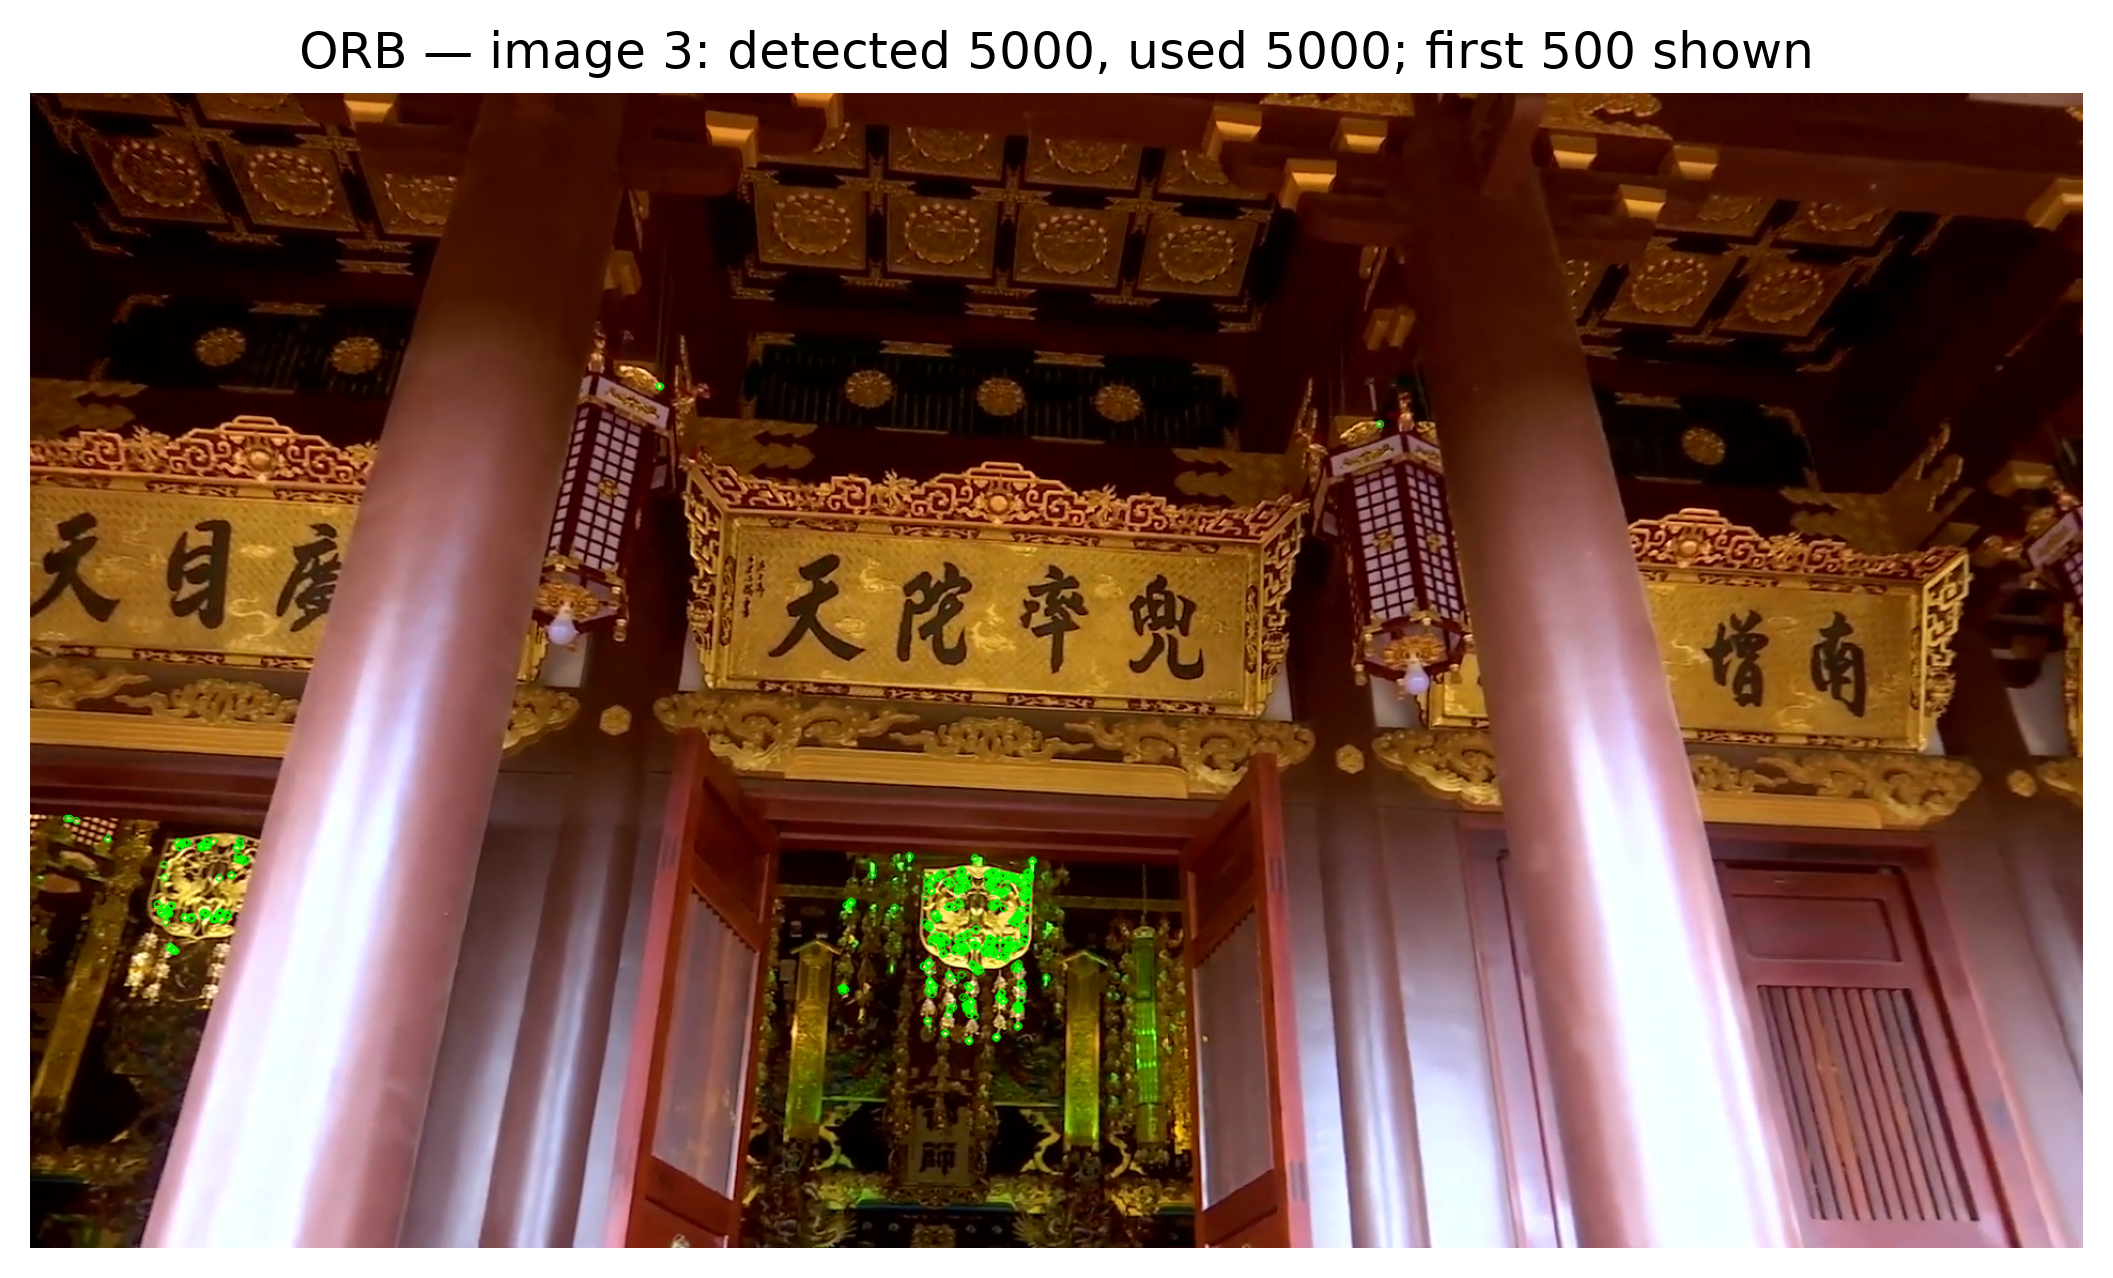
\includegraphics[width=\linewidth]{../results/part_c/refinement/20261019T105909Z_fe7aa242/figures/orb_keypoints_3.png}
\caption{ORB}
\end{subfigure}\hfill
\begin{subfigure}[t]{0.32\textwidth}
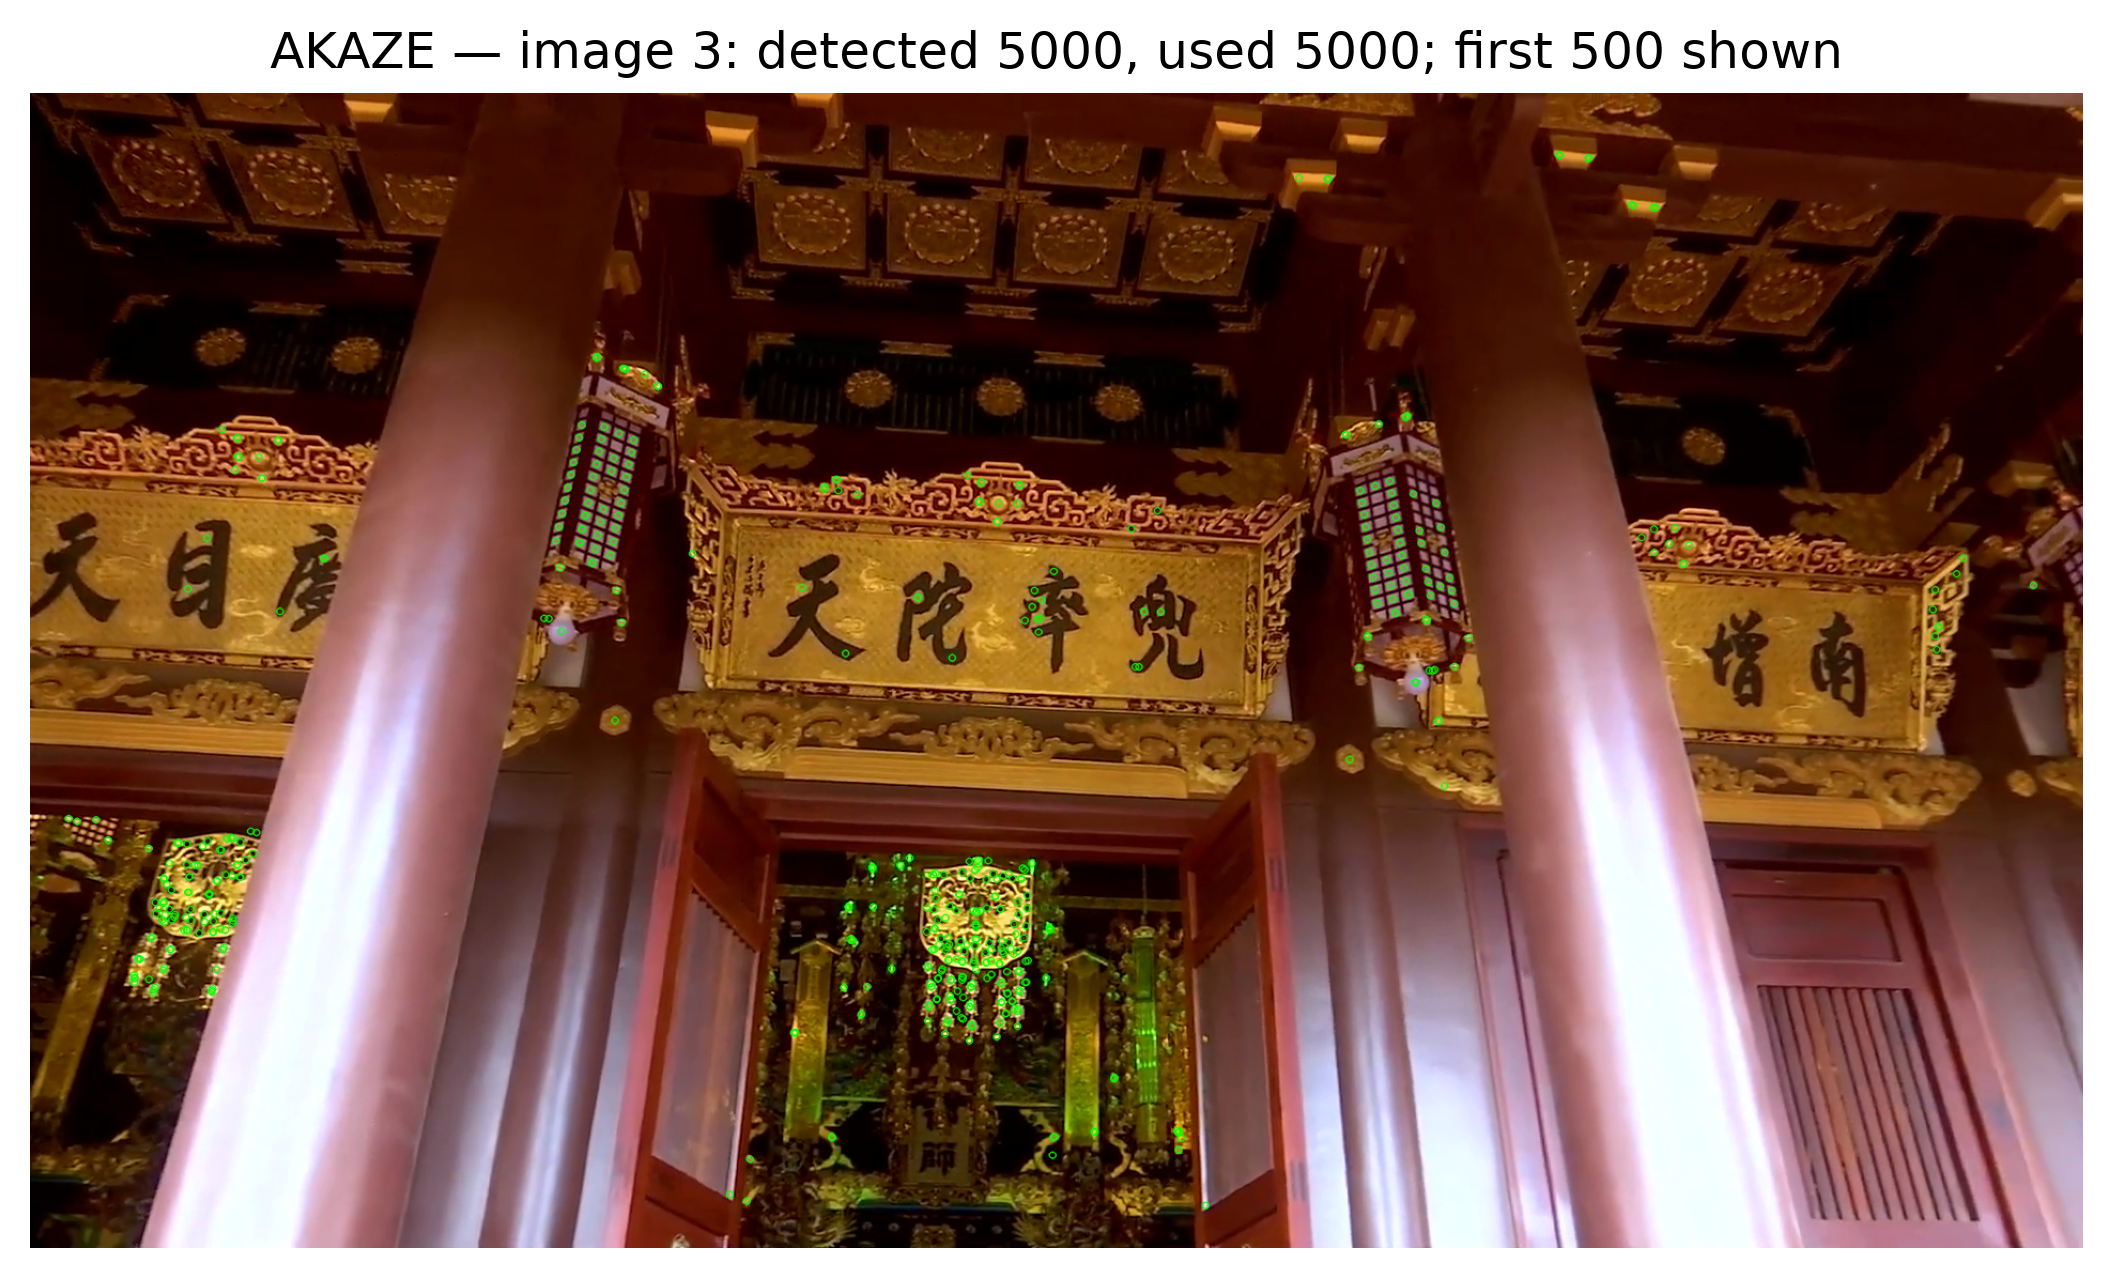
\includegraphics[width=\linewidth]{../results/part_c/refinement/20261019T105909Z_fe7aa242/figures/akaze_keypoints_3.png}
\caption{AKAZE}
\end{subfigure}
\caption{Detected keypoints on image 3. The first 500 retained points are drawn for readability; counts for all four images are in Table~\ref{tab:c-keypoints}.}
\label{fig:c-keypoints}
\end{figure}

\subsubsection{Baseline and selected comparisons}
The common baseline is ratio 0.75 and threshold 3 px. Visual review selected SIFT 0.75/5 px, ORB 0.78/5 px, and AKAZE 0.78/5 px. Table~\ref{tab:c-main} gives the pooled counts, forward reprojection error, and repeated total pipeline time. Initial matches precede the ratio test; the ratio-pass count is shown so the inlier-ratio denominator is explicit.

\begin{table}[htbp]
\centering
\small
\scriptsize
\setlength{\tabcolsep}{3pt}
\caption{Baseline and selected end-to-end stitching results. B and S denote baseline and selected settings. Initial matches count complete KNN rows before Lowe's ratio test; P/R are ratio-pass matches and RANSAC inliers. Each configuration has 15,000 initial matches across the three source-to-anchor pairs. Runtime is the median (IQR) in milliseconds over five repetitions after one warm-up.}
\label{tab:c-main}
\begin{tabular}{llcccrrr}
\toprule
\multicolumn{1}{c}{Detector} & \multicolumn{1}{c}{Param.} & \multicolumn{1}{c}{Features D/U} & \multicolumn{1}{c}{Initial KNN} & \multicolumn{1}{c}{Matches P/R} & \multicolumn{1}{c}{Inlier (\%)} & \multicolumn{1}{c}{RMSE (px)} & \multicolumn{1}{c}{Time (ms)} \\
\midrule
SIFT & B 0.75/3 & 20,001/20,000 & 15,000 & 6,582/5,927 & 90.05 & 0.707 & 2,898.192 (66.391) \\
SIFT & S 0.75/5 & 20,001/20,000 & 15,000 & 6,582/5,950 & 90.40 & 0.726 & 2,838.351 (163.371) \\
ORB & B 0.75/3 & 20,000/20,000 & 15,000 & 5,828/5,332 & 91.49 & 1.215 & 975.079 (39.572) \\
ORB & S 0.78/5 & 20,000/20,000 & 15,000 & 6,442/6,017 & 93.40 & 1.401 & 1,025.075 (69.450) \\
AKAZE & B 0.75/3 & 20,000/20,000 & 15,000 & 6,806/6,416 & 94.27 & 0.832 & 2,114.515 (34.142) \\
AKAZE & S 0.78/5 & 20,000/20,000 & 15,000 & 7,184/6,797 & 94.61 & 0.963 & 1,965.790 (126.001) \\
\bottomrule
\end{tabular}
\end{table}

\begin{figure}[htbp]
\centering
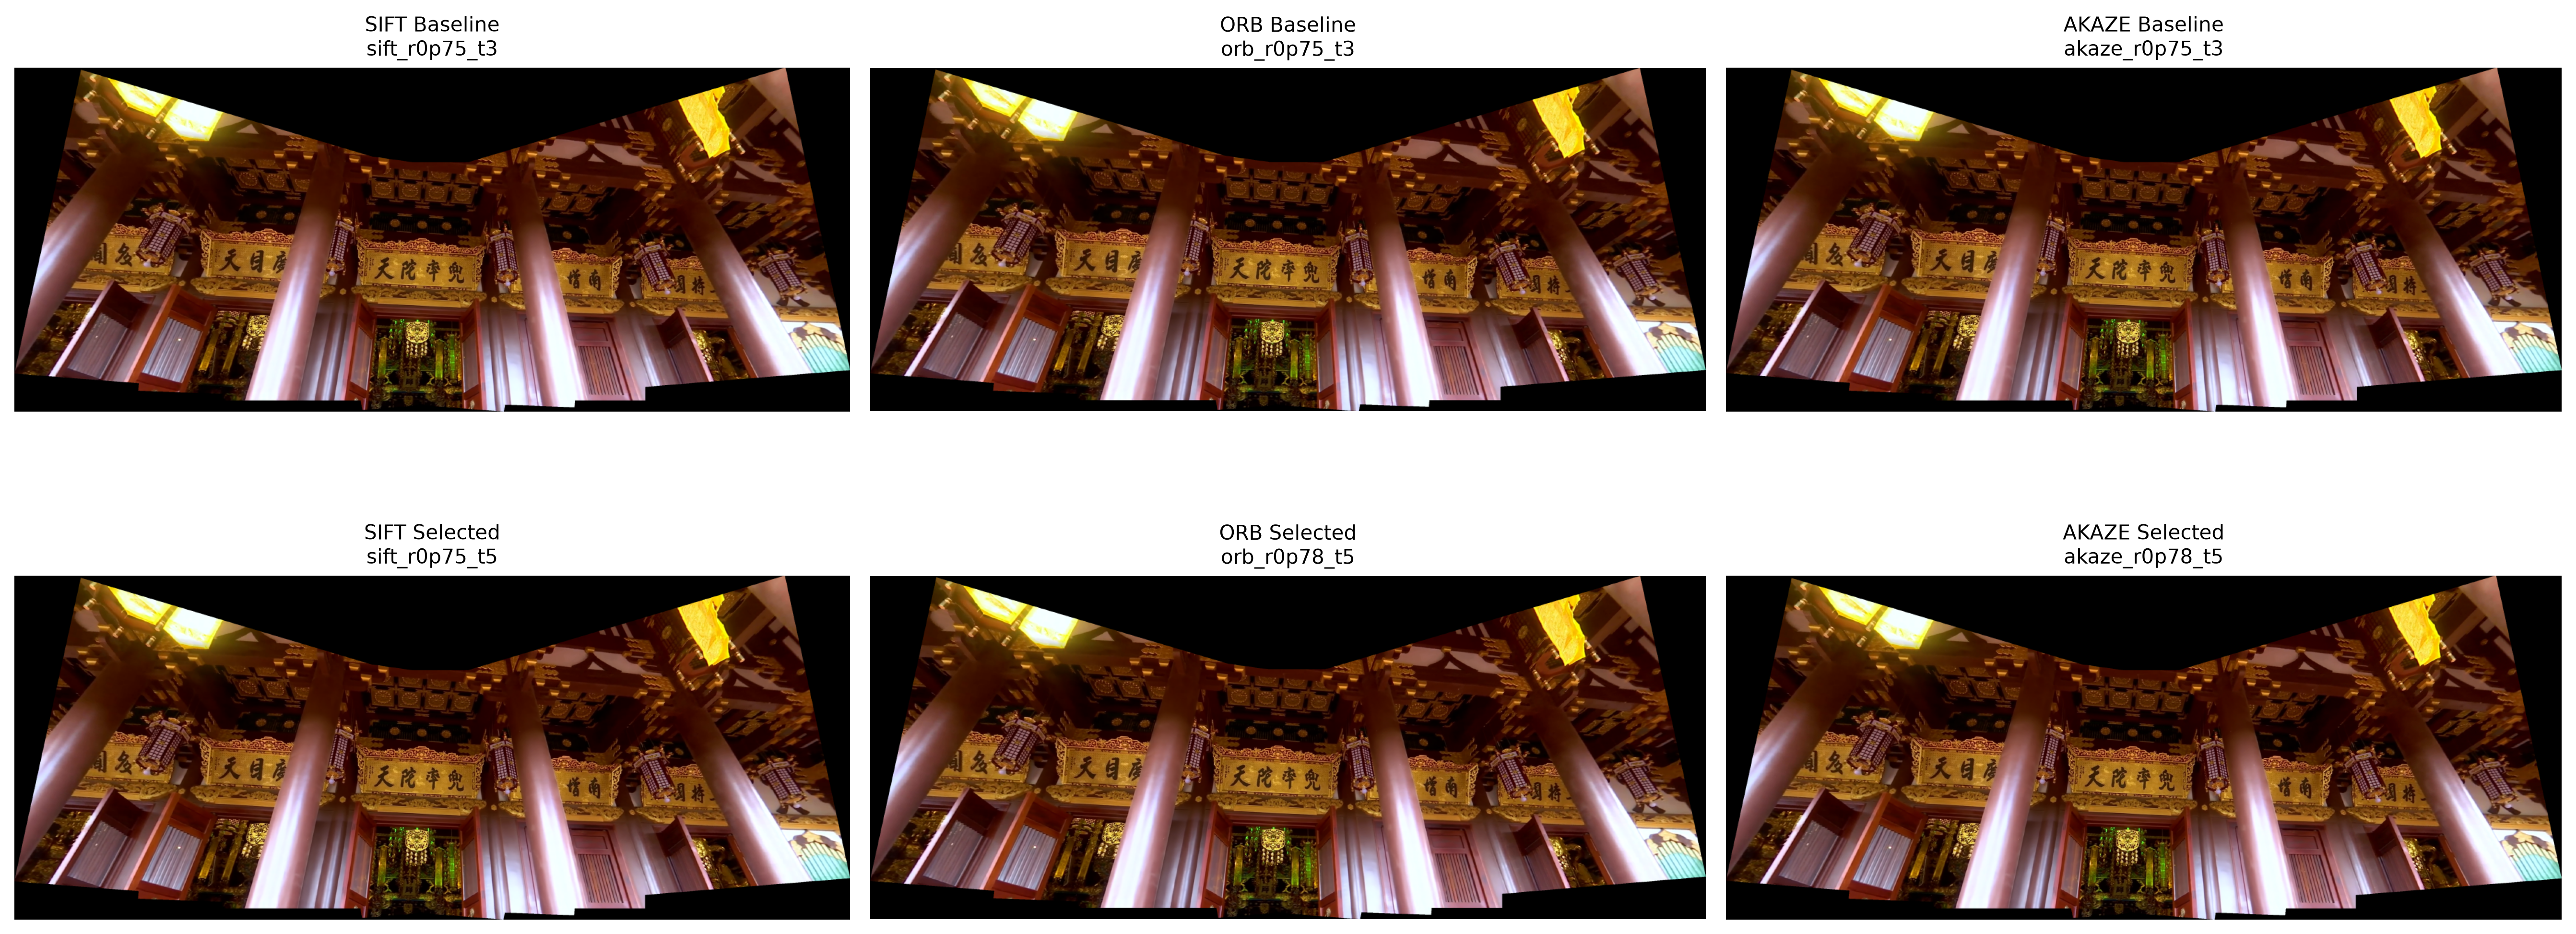
\includegraphics[width=\textwidth]{../results/part_c/refinement/20261019T105909Z_fe7aa242/figures/baseline_selected_panoramas.png}
\caption{Baseline (top) and selected (bottom) feather-blended panoramas for SIFT, ORB, and AKAZE in the image-3 coordinate frame. Black regions lie outside valid image support.}
\label{fig:c-panoramas}
\end{figure}

\begin{figure}[htbp]
\centering
\begin{subfigure}[t]{0.48\textwidth}
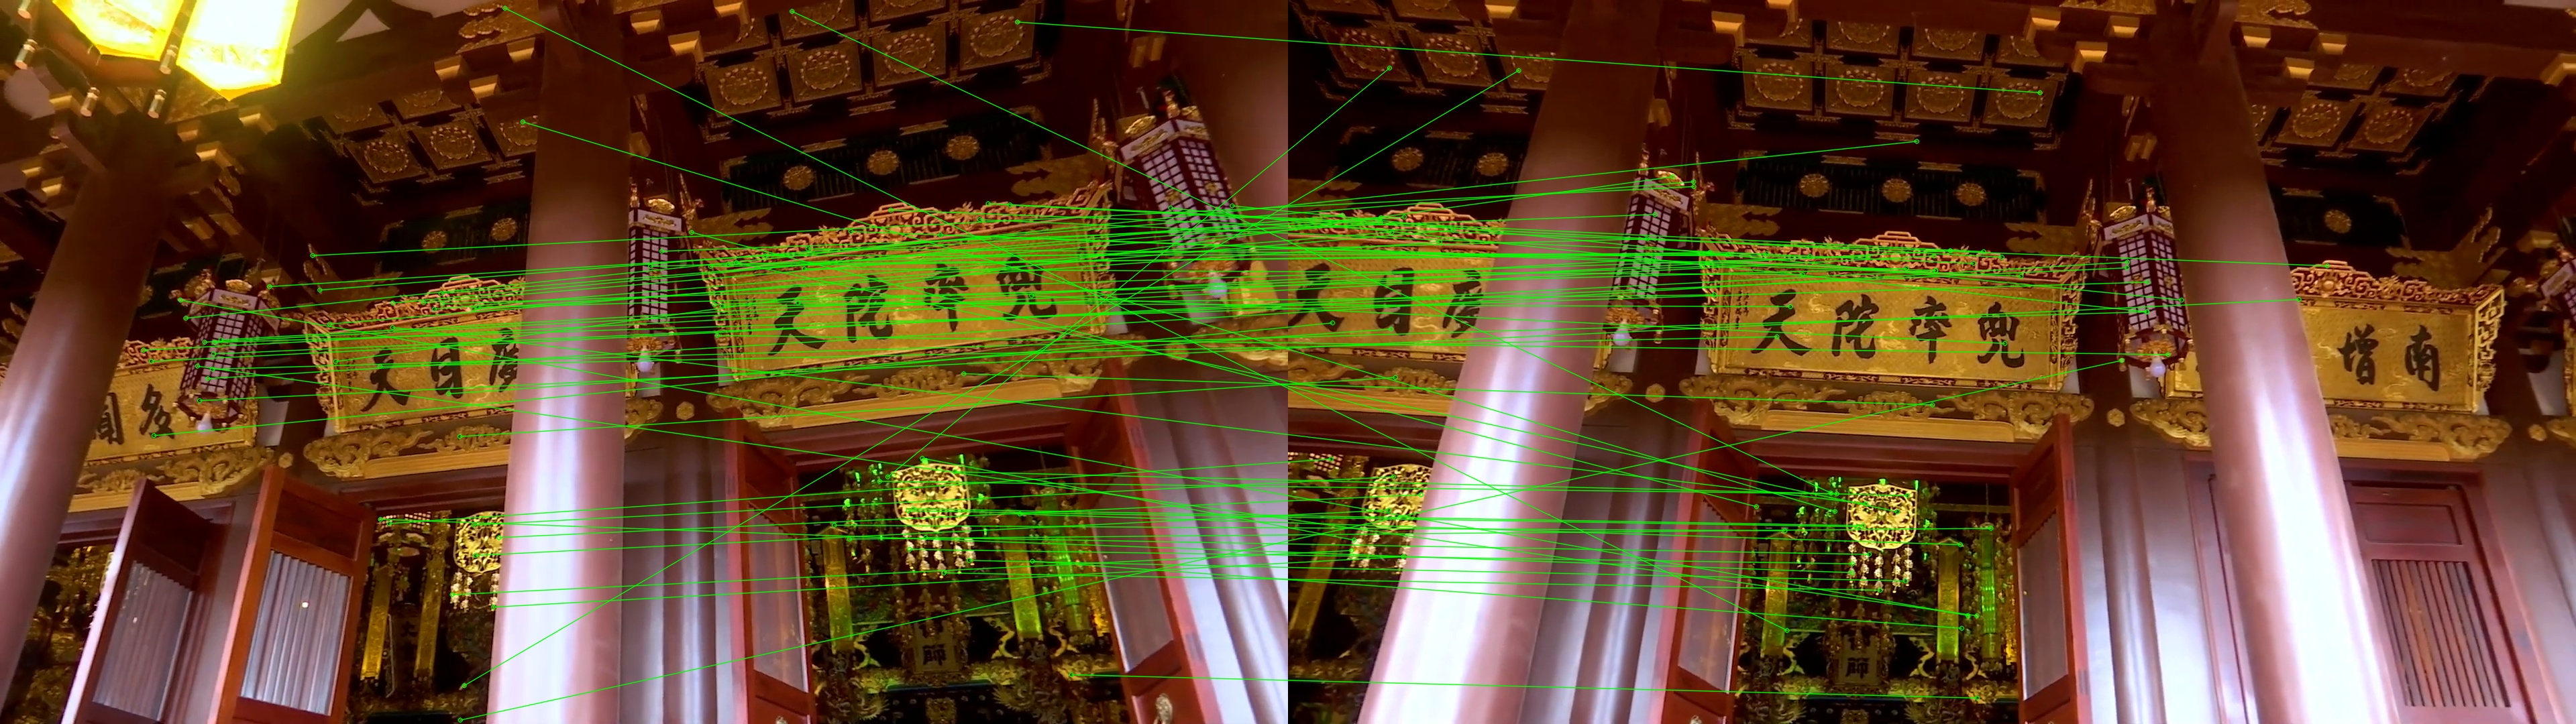
\includegraphics[width=\linewidth]{../results/part_c/refinement/20261019T105909Z_fe7aa242/figures/sift_r0p75_t5_1_to_3_initial.jpg}
\caption{Initial SIFT KNN matches}
\end{subfigure}\hfill
\begin{subfigure}[t]{0.48\textwidth}
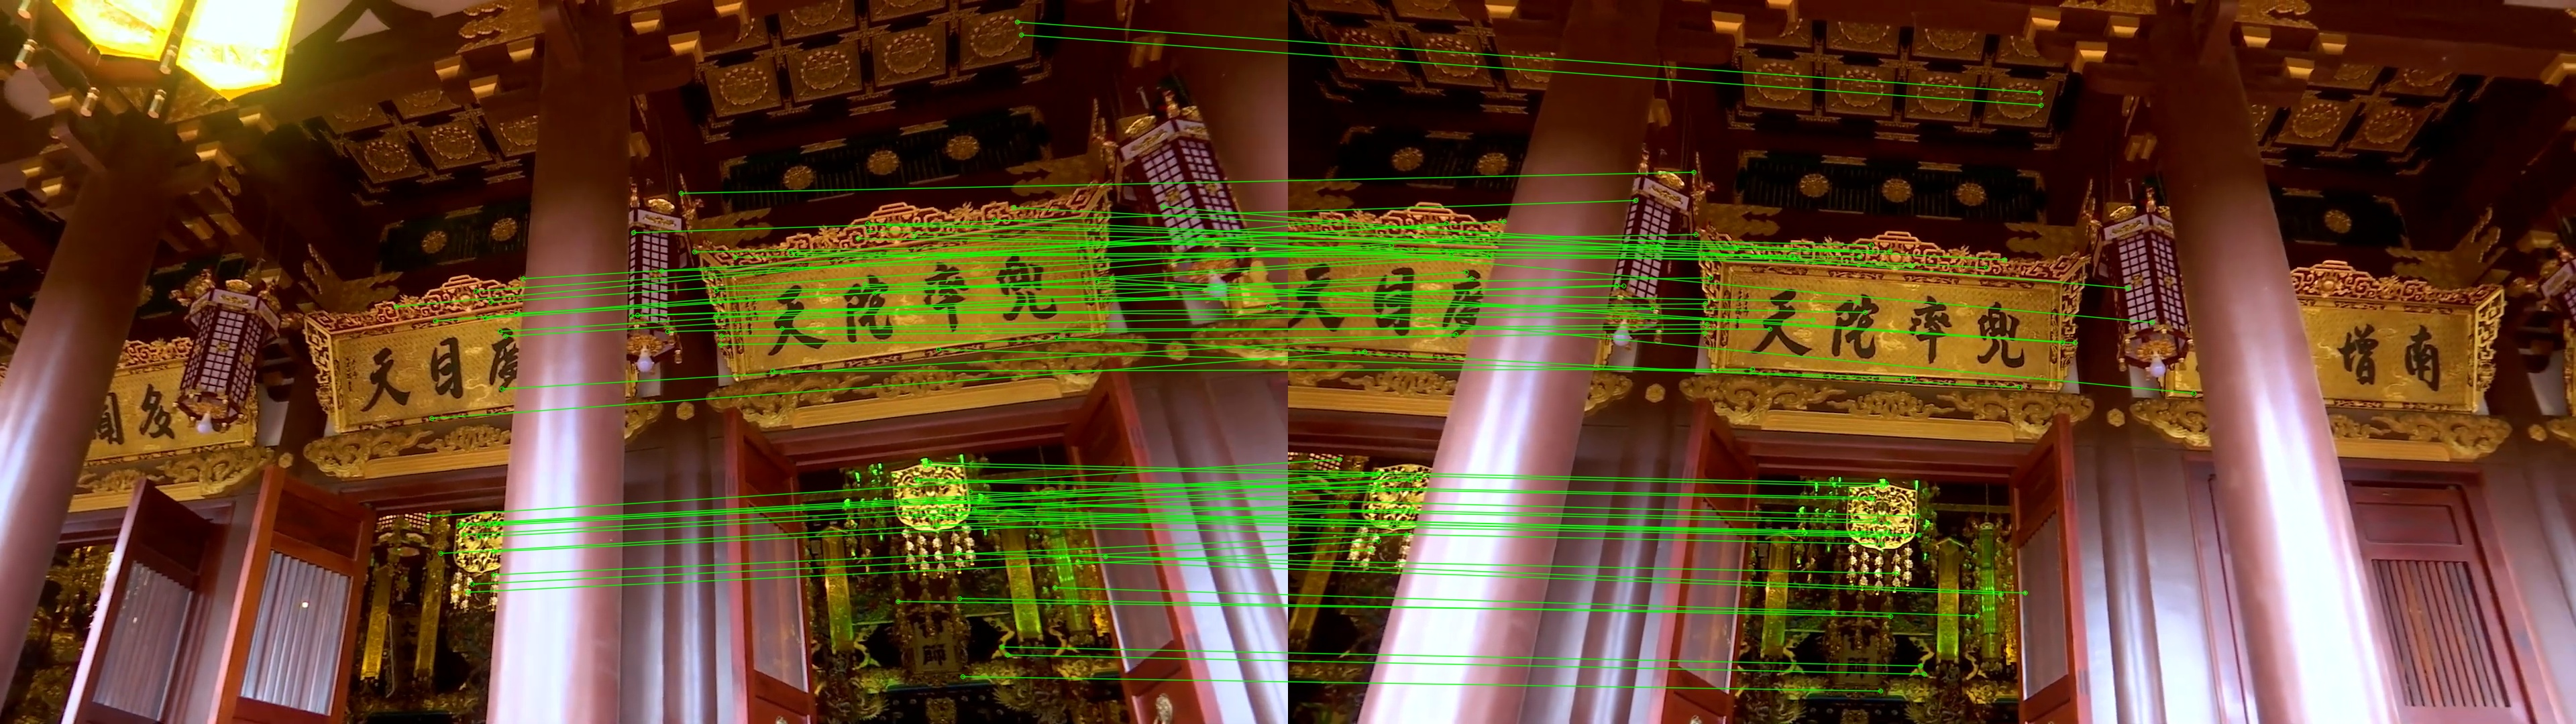
\includegraphics[width=\linewidth]{../results/part_c/refinement/20261019T105909Z_fe7aa242/figures/sift_r0p75_t5_1_to_3_inlier.jpg}
\caption{SIFT RANSAC inliers}
\end{subfigure}
\caption{Example initial and inlier correspondences from image 1 to image 3. Up to 80 matches are drawn for readability; full arrays, homographies, and inlier masks are retained in the run.}
\label{fig:c-matches}
\end{figure}

The selected canvas dimensions are $3793\times1560$ for SIFT, $3779\times1554$ for ORB, and $3791\times1560$ for AKAZE. Selected pooled convex-hull support ranges from 55.52\% to 69.11\% for SIFT, 41.28\% to 44.22\% for ORB, and 53.26\% to 68.55\% for AKAZE across the source and anchor views. This diagnostic shows that the accepted points cover different spatial extents; it does not prove absolute alignment accuracy.

\subsection{Comparative Analysis}

\subsubsection{Parameter sensitivity and geometric stability}
Table~\ref{tab:c-ratio-sensitivity} compares the tested Lowe-ratio endpoints at a fixed 3 px RANSAC threshold. A larger ratio admits more correspondences and inliers but lowers the accepted inlier percentage. Table~\ref{tab:c-threshold-sensitivity} compares 3 px and 6 px thresholds at ratio 0.75. Increasing the threshold accepts additional points and increases fitted RMSE. Corner deviation does not change monotonically with fitted RMSE, so the quantities describe different aspects of the fit.

\begin{table}[htbp]
\centering
\small
\caption{Lowe-ratio endpoints at fixed RANSAC threshold 3 px. Counts pool the three source-to-anchor pairs.}
\label{tab:c-ratio-sensitivity}
\begin{tabular}{lrrr}
\toprule
\multicolumn{1}{c}{Detector} & \multicolumn{1}{c}{\shortstack{Ratio-pass\\matches}} & \multicolumn{1}{c}{Inliers} & \multicolumn{1}{c}{\shortstack{Inlier ratio\\(\%)}} \\
\midrule
SIFT & 6,300$\rightarrow$6,901 & 5,785$\rightarrow$6,078 & 91.83$\rightarrow$88.07 \\
ORB & 5,339$\rightarrow$6,442 & 4,930$\rightarrow$5,741 & 92.34$\rightarrow$89.12 \\
AKAZE & 6,484$\rightarrow$7,184 & 6,168$\rightarrow$6,692 & 95.13$\rightarrow$93.15 \\
\bottomrule
\end{tabular}
\end{table}

\begin{table}[htbp]
\centering
\small
\caption{RANSAC-threshold endpoints at fixed Lowe ratio 0.75. Corner change is the maximum projected-corner deviation observed across three correspondence permutations.}
\label{tab:c-threshold-sensitivity}
\begin{tabular}{lrrr}
\toprule
\multicolumn{1}{c}{Detector} & \multicolumn{1}{c}{Inliers} & \multicolumn{1}{c}{RMSE (px)} & \multicolumn{1}{c}{Max corner change (px)} \\
\midrule
SIFT & 5,927$\rightarrow$5,950 & 0.707$\rightarrow$0.723 px & 4.038$\rightarrow$0.937 px \\
ORB & 5,332$\rightarrow$5,546 & 1.215$\rightarrow$1.406 px & 20.084$\rightarrow$30.301 px \\
AKAZE & 6,416$\rightarrow$6,537 & 0.832$\rightarrow$0.983 px & 12.224$\rightarrow$2.932 px \\
\bottomrule
\end{tabular}
\end{table}

\begin{figure}[htbp]
\centering
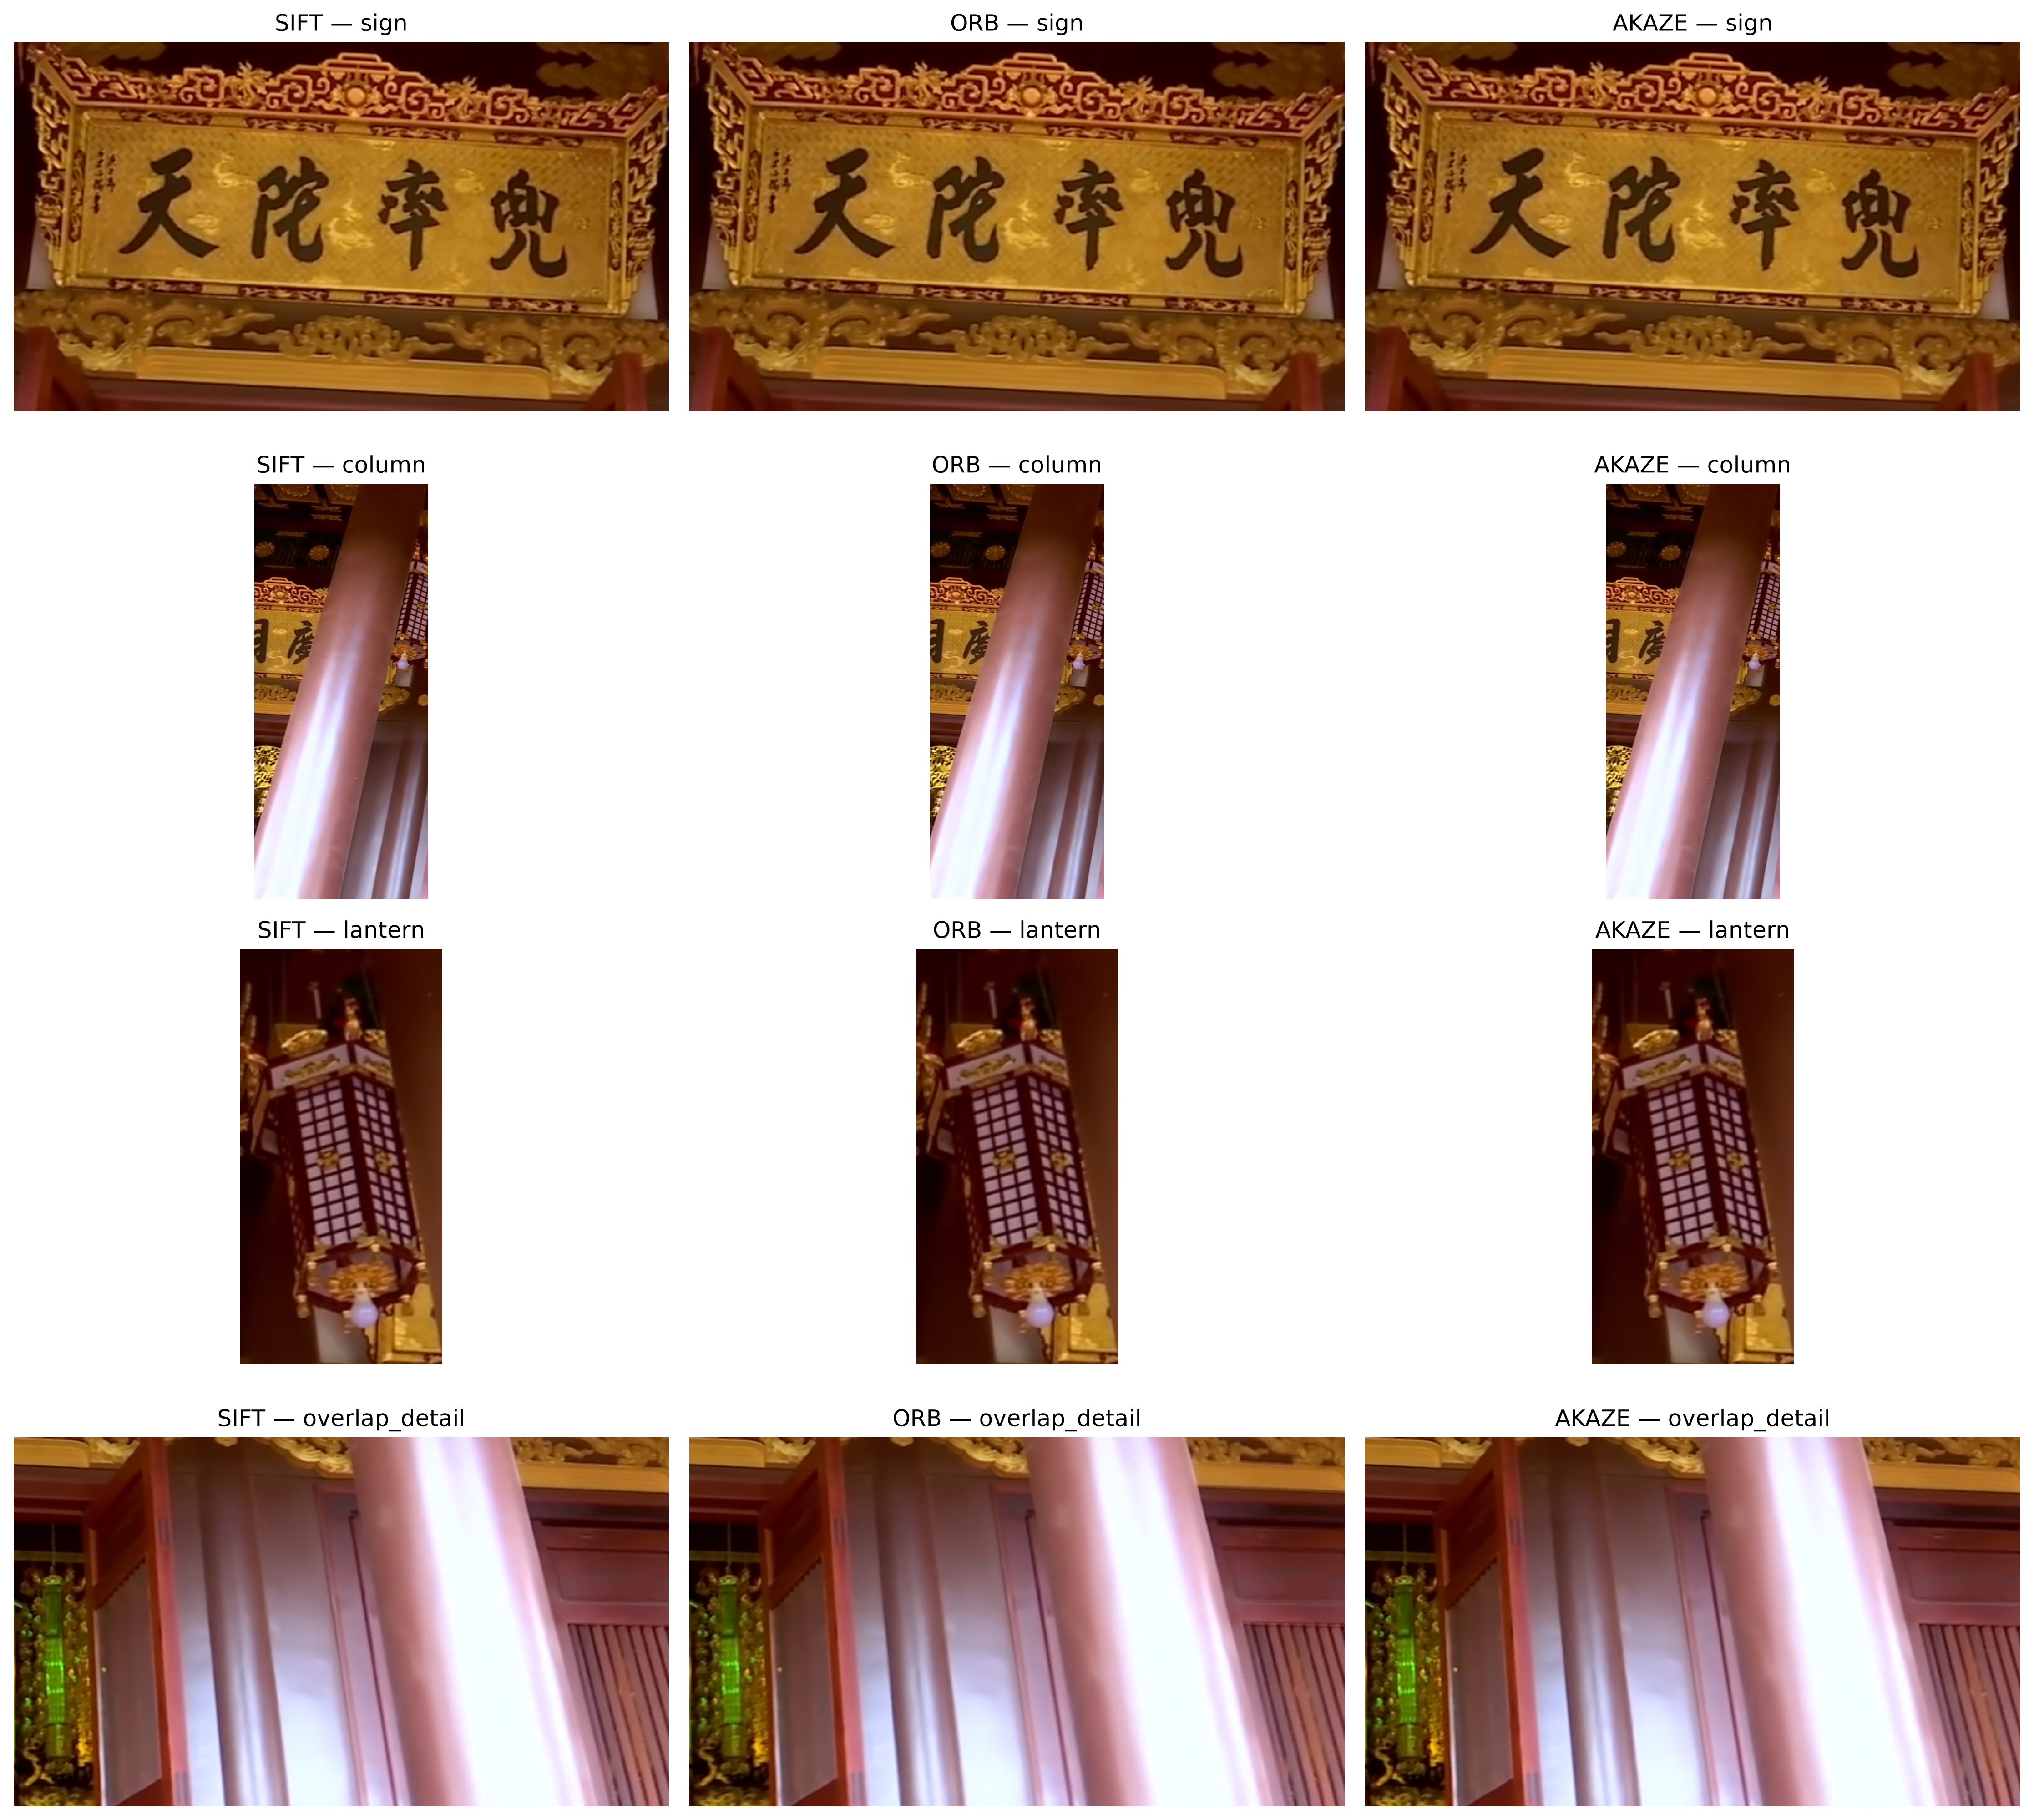
\includegraphics[width=0.88\textwidth]{../results/part_c/refinement/20261019T105909Z_fe7aa242/figures/selected_crop_comparison.png}
\caption{Fixed crops in image-3 coordinates: sign, column, lantern, and overlap detail for the selected detectors.}
\label{fig:c-crops}
\end{figure}

The selected homographies were also refitted from saved correspondences after permutations with NumPy seeds 42, 123, and 2026. Across the three direct source-to-anchor pairs, all 108 homography-and-canvas geometry checks passed. This procedure measures fitted reprojection and projected-corner changes; it does not rerun feature extraction, matching, or blending. Maximum corner changes are 1.565 px for SIFT, 24.328 px for ORB, and 6.038 px for AKAZE. ORB is substantially more sensitive at extrapolated corners despite its high inlier ratio. SIFT gives the lowest selected pooled RMSE and smallest selected corner variation, while AKAZE retains the most selected inliers.

In the inspected native sign crops, lettering and ornament remain continuous across the selected results. Feathering avoids an obvious hard seam at the central sign, while fine overlap detail softens and column ghosting remains visible. The panoramas show leaning outer columns and roof stretching from the planar projection. Bright streaks and saturated yellow highlights persist and are not recovered by changing the blend alone.

\subsubsection{Feather and multi-band blending}
A supplementary experiment holds the selected homographies, support masks, and crop fixed while comparing feathering with 3-, 5-, and 7-band multi-band blending. Table~\ref{tab:c-blending} reports stage-only timing for canvas setup, warping, blending, and cropping. Mean absolute colour change is measured from feathering on common valid support; it is descriptive and not a quality score.

\begin{table}[htbp]
\centering
\small
\setlength{\tabcolsep}{4pt}
\caption{Fixed-homography blending comparison. Time is the median (IQR) over five repetitions after one warm-up.}
\label{tab:c-blending}
\begin{tabular}{llrr}
\toprule
Detector & Blend & Time (ms) & Mean absolute change \\
\midrule
SIFT & Feather & 815.838 (70.504) & 0.000 \\
SIFT & Multi-band, 3 & 1,001.501 (67.641) & 0.662 \\
SIFT & Multi-band, 5 & 1,028.602 (46.028) & 0.779 \\
SIFT & Multi-band, 7 & 1,027.439 (97.292) & 1.315 \\
ORB & Feather & 687.850 (208.455) & 0.000 \\
ORB & Multi-band, 3 & 978.913 (58.832) & 0.738 \\
ORB & Multi-band, 5 & 1,114.966 (43.292) & 0.854 \\
ORB & Multi-band, 7 & 1,238.949 (51.768) & 1.390 \\
AKAZE & Feather & 769.430 (76.210) & 0.000 \\
AKAZE & Multi-band, 3 & 1,196.965 (92.689) & 0.659 \\
AKAZE & Multi-band, 5 & 1,158.733 (41.575) & 0.775 \\
AKAZE & Multi-band, 7 & 1,093.339 (145.709) & 1.312 \\
\bottomrule
\end{tabular}
\end{table}

\begin{figure}[htbp]
\centering
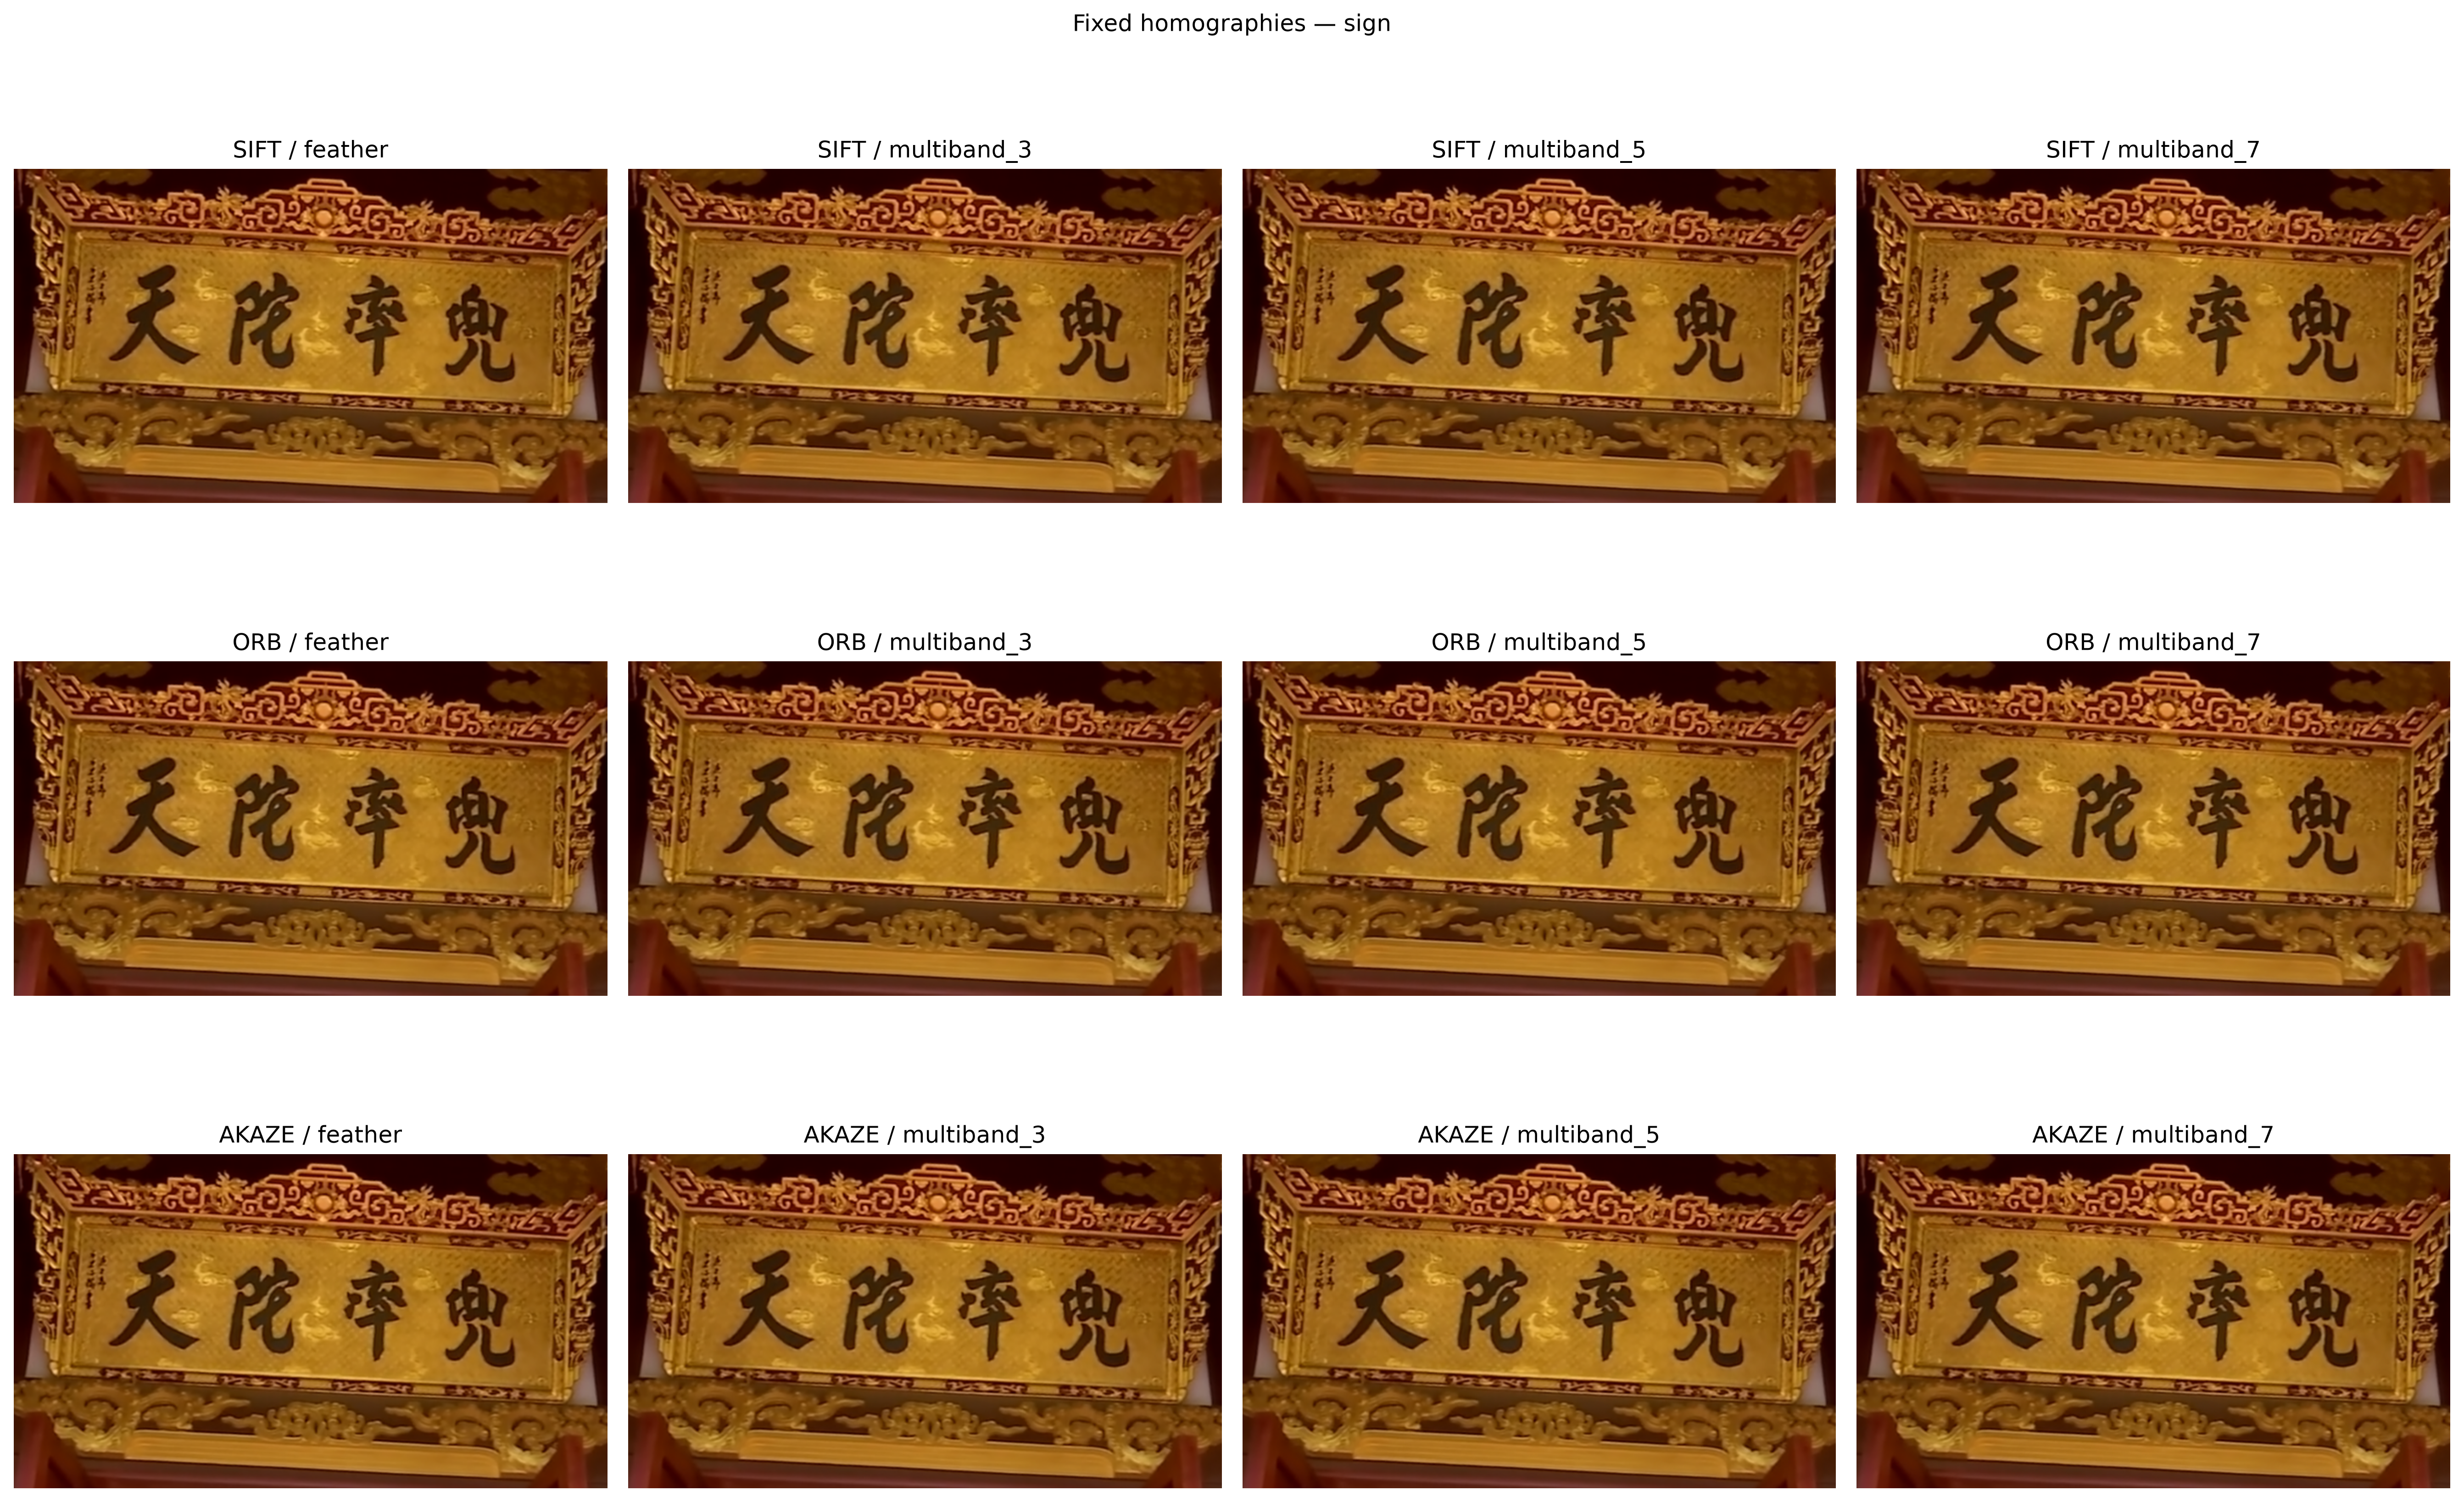
\includegraphics[width=\textwidth]{../results/part_c/refinement/20261019T105909Z_fe7aa242/blending/comparison_sign.png}
\caption{Sign crops from feathering and multi-band blending at fixed homographies. The blending methods preserve similar central lettering while changing local brightness and texture.}
\label{fig:c-blending}
\end{figure}

On the inspected sign, the blending options preserve similar lettering. SIFT 5-band blending takes 1,028.602 ms compared with 815.838 ms for feathering in the separate stage-only measurement. Seven bands produce the largest mean colour change for each detector, but neither this change nor the band count shows a quality improvement. Feathering remains the shared baseline for the detector comparison. Multi-band blending does not remove projective stretching or recover saturated detail.

Overall, ORB has the lowest selected total stitching time at 1,025.075 ms, SIFT has the lowest selected pooled reprojection RMSE at 0.726 px and the smallest tested corner variation, and AKAZE retains the most selected inliers at 6,797 (94.61\%). These results show distinct speed, fit, and support trade-offs on this four-image sequence. They do not establish performance on other scenes or absolute geometric accuracy.

\section{Conclusion}
Across the tested inputs, classical methods produced clear but task-dependent results. Gaussian filtering gave the strongest PSNR for Gaussian noise, while median filtering best suppressed salt-and-pepper noise; sharpening gains were modest and parameter-sensitive. On the Venus pair, SGBM improved disparity coverage and error over BM at a higher runtime. For stitching, SIFT gave the most stable geometric fit, ORB was fastest but more sensitive at extrapolated corners, and AKAZE retained the most inliers. The reconstructed point clouds remain qualitative because the camera model is assumed.

Further work should use measured stereo calibration and occlusion-aware ground truth, then evaluate additional scenes. Filtering could be tested on more reference images and noise distributions, including edge-aware methods. For stitching, exposure compensation and local or non-planar alignment may address illumination changes and perspective distortion; more sequences are needed to determine whether the observed detector trade-offs generalize.

\section{References}
\begingroup
\small
\sloppy
\raggedright
\setlength{\parskip}{0pt}
\begin{enumerate}[label={[\arabic*]},leftmargin=*,itemsep=0.25em,topsep=0.25em,parsep=0pt]
\item OpenCV. ``Image Filtering.'' OpenCV 4.x API Reference. \url{https://docs.opencv.org/4.x/d4/d86/group__imgproc__filter.html}.
\item OpenCV. ``Laplace Operator.'' OpenCV 4.x Tutorials. \url{https://docs.opencv.org/4.x/d5/db5/tutorial_laplace_operator.html}.
\item scikit-image contributors. ``skimage.metrics.structural\_similarity.'' API Reference. \url{https://scikit-image.org/docs/stable/api/skimage.metrics.html#skimage.metrics.structural_similarity}.
\item Middlebury College. ``Optical Flow: Other Datasets.'' \url{https://vision.middlebury.edu/flow/data/}.
\item Middlebury College. ``Venus Stereo Data Archive.'' \url{https://vision.middlebury.edu/stereo/data/scenes2001/data/venus/venus.zip}.
\item OpenCV. ``USAC: Universal RANSAC.'' OpenCV 4.x Tutorials. \url{https://docs.opencv.org/4.x/de/d3e/tutorial_usac.html}.
\item OpenCV. ``Camera Calibration and 3D Reconstruction.'' OpenCV 4.x API Reference, calib3d module. \url{https://docs.opencv.org/4.x/d9/d0c/group__calib3d.html}.
\item OpenCV. ``Stereo Correspondence.'' OpenCV 5.0 API Reference. \url{https://docs.opencv.org/5.0/main_modules/stereo.html}.
\item D. Scharstein and R. Szeliski, ``A Taxonomy and Evaluation of Dense Two-Frame Stereo Correspondence Algorithms,'' \emph{International Journal of Computer Vision}, vol. 47, pp. 7--42, 2002. \url{https://doi.org/10.1023/A:1014573219977}.
\item T. Basha, Y. Moses, and N. Kiryati, ``Multi-view Scene Flow Estimation: A View Centered Variational Approach,'' \emph{International Journal of Computer Vision}, vol. 101, pp. 6--21, 2013. \url{https://doi.org/10.1007/s11263-012-0542-7}.
\end{enumerate}
\endgroup

\appendix
\section{Appendix: Python Code}
\lstset{basicstyle=\ttfamily\footnotesize}
\subsection{Part A: Image Filtering}
The excerpts below show the core Part A algorithms and metrics. They omit input checks and run orchestration; the accompanying source package contains the complete executable implementation.
\begin{lstlisting}
import hashlib
import math
import cv2
import numpy as np
from skimage.metrics import structural_similarity

def make_noisy_image(reference, noise_type, noise_level, seed):
    noise_code = 0 if noise_type == "gaussian" else 1
    level_digest = hashlib.sha256(float(noise_level).hex().encode()).digest()
    level_code = int.from_bytes(level_digest[:8], "big")
    rng = np.random.default_rng(np.random.SeedSequence([seed, noise_code, level_code]))
    if noise_type == "gaussian":
        noise = rng.normal(0, noise_level, reference.shape)
        return np.rint(np.clip(reference.astype(np.float64) + noise, 0, 255)).astype(np.uint8)

    height, width = reference.shape[:2]
    count = round(noise_level * height * width)
    indices = rng.choice(height * width, size=count, replace=False)
    salt_count = round(count / 2)
    result = reference.copy()
    flat = result.reshape(-1, 3)
    flat[indices[:salt_count]] = 255
    flat[indices[salt_count:]] = 0
    return result

def denoise(image, method, kernel_size, sigma=None):
    if method == "mean":
        return cv2.blur(image, (kernel_size, kernel_size), borderType=cv2.BORDER_REPLICATE)
    if method == "gaussian":
        return cv2.GaussianBlur(image, (kernel_size, kernel_size),
                                sigmaX=sigma, sigmaY=sigma,
                                borderType=cv2.BORDER_REPLICATE)
    return cv2.medianBlur(image, kernel_size)

def sharpen_laplacian(image, laplacian_kernel_size, alpha):
    working = image.astype(np.float32)
    scale = 2.0 ** (4 - 2 * laplacian_kernel_size)
    laplacian = cv2.Laplacian(working, cv2.CV_32F,
                              ksize=laplacian_kernel_size, scale=scale,
                              borderType=cv2.BORDER_REPLICATE)
    return np.rint(np.clip(working - alpha * laplacian, 0, 255)).astype(np.uint8)

def compute_metrics(reference, result):
    difference = reference.astype(np.float64) - result.astype(np.float64)
    mse = float(np.mean(difference ** 2))
    psnr = math.inf if mse == 0 else 10 * math.log10(255 ** 2 / mse)
    ssim = structural_similarity(
        reference, result, data_range=255, channel_axis=-1,
        gaussian_weights=True, sigma=1.5, use_sample_covariance=False
    )
    return {"mse": mse, "psnr_db": psnr, "ssim": float(ssim)}
\end{lstlisting}
\clearpage
\subsection{Part B: 3D Reconstruction}
The excerpt shows feature matching and RANSAC estimation, BM/SGBM disparity computation, ground-truth evaluation, and reprojection. The Venus disparity ground truth is derived from horizontal flow for the verified rectified pair. The camera model is assumed, so the point cloud has normalized baseline units and is qualitative rather than metric.
\begin{lstlisting}
import cv2
import numpy as np

def estimate_fundamental(left, right, threshold):
    sift = cv2.SIFT_create(nfeatures=5000)
    kp_l, des_l = sift.detectAndCompute(left, None)
    kp_r, des_r = sift.detectAndCompute(right, None)
    pairs = cv2.BFMatcher(cv2.NORM_L2).knnMatch(des_l, des_r, k=2)
    good = [m for m, n in pairs if m.distance < 0.75 * n.distance]
    pts_l = np.float32([kp_l[m.queryIdx].pt for m in good])
    pts_r = np.float32([kp_r[m.trainIdx].pt for m in good])
    cv2.setRNGSeed(42)
    F, inliers = cv2.findFundamentalMat(
        pts_l, pts_r, cv2.USAC_MAGSAC, threshold, 0.999, 5000)
    return F, pts_l, pts_r, inliers.ravel().astype(bool)

def matcher(method, disparities, block, minimum):
    if method == "bm":
        stereo = cv2.StereoBM_create(disparities, block)
        stereo.setMinDisparity(minimum)
        stereo.setTextureThreshold(10)
        stereo.setPreFilterType(cv2.STEREO_BM_PREFILTER_XSOBEL)
        stereo.setPreFilterSize(9)
    else:
        stereo = cv2.StereoSGBM_create(
            minimum, disparities, block, P1=8 * block ** 2,
            P2=32 * block ** 2, mode=cv2.STEREO_SGBM_MODE_SGBM_3WAY)
    stereo.setUniquenessRatio(10)
    stereo.setPreFilterCap(31)
    stereo.setSpeckleWindowSize(0)
    stereo.setSpeckleRange(0)
    stereo.setDisp12MaxDiff(1_000_000)
    return stereo

def compute_disparity(left, right, method, disparities, block, minimum=-16):
    gray_left = cv2.cvtColor(left, cv2.COLOR_BGR2GRAY)
    gray_right = cv2.cvtColor(right, cv2.COLOR_BGR2GRAY)
    minimum_r = -minimum - disparities + 1
    raw_l = matcher(method, disparities, block, minimum).compute(gray_left, gray_right)
    raw_r = matcher(method, disparities, block, minimum_r).compute(gray_right, gray_left)
    d_l, d_r = raw_l.astype(np.float32) / 16, raw_r.astype(np.float32) / 16
    valid_l = (raw_l > (minimum - 1) * 16) & (d_l >= minimum) & (d_l < minimum + disparities)
    valid_r = (raw_r > (minimum_r - 1) * 16) & (d_r >= minimum_r) & (d_r < minimum_r + disparities)
    y, x = np.indices(d_l.shape)
    x_r = x - d_l
    inside = valid_l & (x_r >= 0) & (x_r <= d_l.shape[1] - 1)
    nearest = np.clip(np.rint(x_r).astype(int), 0, d_l.shape[1] - 1)
    consistent = inside & valid_r[y, nearest] & (np.abs(d_l + d_r[y, nearest]) <= 1.0)
    return d_l, consistent

def flow_ground_truth(flow):
    valid = np.isfinite(flow).all(axis=2) & (np.abs(flow) <= 1e9).all(axis=2)
    valid &= np.abs(flow[:, :, 1]) <= 1e-4
    y, x = np.indices(valid.shape)
    x_r, y_r = x + flow[:, :, 0], y + flow[:, :, 1]
    inside = ((x_r >= 0) & (x_r < valid.shape[1]) &
              (y_r >= 0) & (y_r < valid.shape[0]))
    return -flow[:, :, 0].astype(np.float32), valid & inside

def disparity_metrics(disparity, lr_valid, gt_disparity, gt_domain):
    error = np.abs(disparity.astype(np.float64) - gt_disparity)
    values = error[lr_valid & gt_domain]
    rmse = np.sqrt(np.mean(values ** 2)) if values.size else None
    bad_pct = 100 * np.mean(values > 1.0) if values.size else None
    return rmse, bad_pct

def reproject(disparity, valid, reprojection_matrix):
    points = cv2.reprojectImageTo3D(disparity.astype(np.float32), reprojection_matrix)
    valid = valid & np.isfinite(points).all(axis=2) & (points[:, :, 2] > 0)
    points[~valid] = np.nan
    return points, valid
\end{lstlisting}

\clearpage
\subsection{Part C: Image Stitching}
The excerpt shows feature detection, KNN matching with Lowe's ratio test, RANSAC homographies to image 3, and distance-transform feather blending. Input loading, failure handling, and experiment bookkeeping are omitted.
\begin{lstlisting}
import cv2
import numpy as np

def create_detector(method, maximum=5000):
    if method == "sift":
        return cv2.SIFT_create(nfeatures=maximum), cv2.NORM_L2
    if method == "orb":
        return cv2.ORB_create(nfeatures=maximum, WTA_K=2), cv2.NORM_HAMMING
    return (cv2.xfeatures2d.AKAZE_create(threshold=0.001, max_points=maximum),
            cv2.NORM_HAMMING)

def extract_features(images, method):
    detector, norm = create_detector(method)
    features = []
    for image in images:
        gray = cv2.cvtColor(image, cv2.COLOR_BGR2GRAY)
        keypoints, descriptors = detector.detectAndCompute(gray, None)
        order = sorted(range(len(keypoints)),
                       key=lambda i: -keypoints[i].response)[:5000]
        features.append(([keypoints[i] for i in order], descriptors[order]))
    return features, norm

def match_features(source, destination, norm, ratio=0.75):
    key_s, desc_s = source
    key_d, desc_d = destination
    pairs = cv2.BFMatcher(norm, crossCheck=False).knnMatch(desc_s, desc_d, k=2)
    complete = [pair for pair in pairs if len(pair) == 2]
    good = [first for first, second in complete
            if first.distance < ratio * second.distance]
    points_s = np.float32([key_s[m.queryIdx].pt for m in good])
    points_d = np.float32([key_d[m.trainIdx].pt for m in good])
    return points_s, points_d, len(complete), len(good)

def estimate_homography(points_s, points_d, threshold):
    H, mask = cv2.findHomography(
        points_s, points_d, cv2.RANSAC, threshold,
        maxIters=5000, confidence=0.995)
    inliers = mask.ravel().astype(bool)
    H = H / H[2, 2]
    projected = cv2.perspectiveTransform(
        points_s[inliers].reshape(-1, 1, 2), H).reshape(-1, 2)
    rmse = np.sqrt(np.mean(np.sum((projected - points_d[inliers]) ** 2, axis=1)))
    return H, inliers, rmse

def stitch_four(images, method, ratio=0.75, threshold=3.0):
    features, norm = extract_features(images, method)
    anchor = 2
    transforms = [np.eye(3) for _ in images]
    pair_results = []
    for index in (0, 1, 3):
        source, destination, initial, passed = match_features(
            features[index], features[anchor], norm, ratio)
        H, inliers, rmse = estimate_homography(source, destination, threshold)
        transforms[index] = H
        inlier_count = int(inliers.sum())
        pair_results.append((initial, passed, inlier_count,
                             100 * inlier_count / passed, rmse))
    panorama = feather_blend(images, transforms)
    return panorama, pair_results

def feather_blend(images, transforms):
    corners = []
    for image, H in zip(images, transforms):
        h, w = image.shape[:2]
        xy = np.float32([[0, 0], [w, 0], [w, h], [0, h]]).reshape(-1, 1, 2)
        corners.append(cv2.perspectiveTransform(xy, H).reshape(-1, 2))
    all_corners = np.concatenate(corners)
    lower = np.floor(all_corners.min(axis=0))
    upper = np.ceil(all_corners.max(axis=0))
    width, height = (upper - lower).astype(int)
    translate = np.array([[1, 0, -lower[0]], [0, 1, -lower[1]], [0, 0, 1]])
    color_sum = np.zeros((height, width, 3), np.float32)
    weight_sum = np.zeros((height, width), np.float32)
    for image, H in zip(images, transforms):
        mask = np.pad(np.ones(image.shape[:2], np.uint8), 1)
        weight = cv2.distanceTransform(mask, cv2.DIST_L2,
                                       cv2.DIST_MASK_PRECISE)[1:-1, 1:-1]
        weight /= weight.max()
        matrix = translate @ H
        color_sum += cv2.warpPerspective(
            image.astype(np.float32) * weight[:, :, None], matrix,
            (width, height), flags=cv2.INTER_LINEAR)
        weight_sum += cv2.warpPerspective(weight, matrix, (width, height))
    valid = weight_sum > 1e-8
    np.divide(
        color_sum, weight_sum[:, :, None], out=color_sum,
        where=valid[:, :, None]
    )
    panorama = np.rint(np.clip(color_sum, 0, 255)).astype(np.uint8)
    y, x = np.nonzero(valid)
    return panorama[y.min():y.max()+1, x.min():x.max()+1]
\end{lstlisting}
\clearpage
\section{Part A: Complete Final-Grid Results}
\label{app:a-full}
These tables reproduce all 528 configuration groups from the final Part A run.\par
Source: \texttt{20261019T024705Z\_aef5c7be/summary.csv}.\par Quality is mean $\pm$ sample standard deviation over seeds 42, 43, and 44. Time is median (IQR), in ms, over 30 samples per processed configuration; noisy inputs have no processing runtime. The earlier parameter-search experiments are outside this final grid.
Configuration notation: M = mean, G = Gaussian, Med = median; $k$ is denoising kernel width and $s$ is Gaussian filter sigma. $+L(k,a)$ denotes denoising followed by Laplacian aperture $k$ and strength $a$; L alone denotes direct sharpening of the noisy input. Laplacian scale is $2^{4-2k}$. All kernel sizes are square.
\subsection{Gaussian noise: standard deviation 10}
\begingroup
\footnotesize
\setlength{\tabcolsep}{4pt}
\begin{longtable}{lrrrr}
\caption{Complete final-grid results: Gaussian noise, $\sigma_n=10$.}\\
\toprule Configuration & PSNR (dB) & SSIM & MSE & Time (ms) \\ \midrule
\endfirsthead
\toprule Configuration & PSNR (dB) & SSIM & MSE & Time (ms) \\ \midrule
\endhead
\midrule \multicolumn{5}{r}{Continued on next page}\\
\endfoot
\bottomrule
\endlastfoot
Noisy input & 28.2319 $\pm$ 0.0001 & 0.54723 $\pm$ 0.00010 & 97.70 $\pm$ 0.00 & N/A \\
M 3 & 33.7557 $\pm$ 0.0018 & 0.87724 $\pm$ 0.00005 & 27.38 $\pm$ 0.01 & 0.422 (0.037) \\
M 3 + L(3, 0.1) & 33.6172 $\pm$ 0.0012 & 0.85861 $\pm$ 0.00007 & 28.27 $\pm$ 0.01 & 8.714 (1.424) \\
M 3 + L(3, 0.2) & 33.3516 $\pm$ 0.0008 & 0.83704 $\pm$ 0.00007 & 30.06 $\pm$ 0.01 & 7.967 (2.712) \\
M 3 + L(3, 0.25) & 33.1784 $\pm$ 0.0011 & 0.82555 $\pm$ 0.00009 & 31.28 $\pm$ 0.01 & 7.387 (1.201) \\
M 3 + L(3, 0.5) & 32.0252 $\pm$ 0.0029 & 0.76279 $\pm$ 0.00018 & 40.79 $\pm$ 0.03 & 8.328 (1.495) \\
M 3 + L(5, 0.1) & 33.9140 $\pm$ 0.0010 & 0.87715 $\pm$ 0.00002 & 26.40 $\pm$ 0.01 & 9.435 (1.170) \\
M 3 + L(5, 0.2) & 33.8397 $\pm$ 0.0004 & 0.86593 $\pm$ 0.00002 & 26.86 $\pm$ 0.00 & 10.166 (2.778) \\
M 3 + L(5, 0.25) & 33.8103 $\pm$ 0.0004 & 0.86137 $\pm$ 0.00003 & 27.04 $\pm$ 0.00 & 9.484 (1.177) \\
M 3 + L(5, 0.5) & 33.5633 $\pm$ 0.0027 & 0.84176 $\pm$ 0.00006 & 28.63 $\pm$ 0.02 & 9.707 (1.516) \\
M 3 + L(7, 0.1) & 33.8914 $\pm$ 0.0017 & 0.87799 $\pm$ 0.00004 & 26.54 $\pm$ 0.01 & 10.874 (1.646) \\
M 3 + L(7, 0.2) & 33.9027 $\pm$ 0.0005 & 0.87361 $\pm$ 0.00002 & 26.47 $\pm$ 0.00 & 11.124 (1.182) \\
M 3 + L(7, 0.25) & 33.8703 $\pm$ 0.0004 & 0.86960 $\pm$ 0.00002 & 26.67 $\pm$ 0.00 & 11.668 (1.360) \\
M 3 + L(7, 0.5) & 33.7212 $\pm$ 0.0013 & 0.85517 $\pm$ 0.00003 & 27.60 $\pm$ 0.01 & 10.640 (1.145) \\
M 5 & 31.5249 $\pm$ 0.0038 & 0.89101 $\pm$ 0.00010 & 45.77 $\pm$ 0.04 & 0.546 (0.110) \\
M 7 & 29.6966 $\pm$ 0.0024 & 0.87008 $\pm$ 0.00003 & 69.73 $\pm$ 0.04 & 1.384 (0.810) \\
M 9 & 28.3464 $\pm$ 0.0025 & 0.84862 $\pm$ 0.00005 & 95.16 $\pm$ 0.06 & 1.557 (0.857) \\
M 11 & 27.2953 $\pm$ 0.0026 & 0.83092 $\pm$ 0.00004 & 121.21 $\pm$ 0.07 & 1.059 (0.631) \\
G 3 / 0.6 & 33.4188 $\pm$ 0.0012 & 0.80630 $\pm$ 0.00007 & 29.59 $\pm$ 0.01 & 0.660 (0.118) \\
G 3 / 0.8 & 34.2654 $\pm$ 0.0010 & 0.86351 $\pm$ 0.00001 & 24.35 $\pm$ 0.01 & 0.643 (0.165) \\
G 3 / 1.0 & 34.2581 $\pm$ 0.0010 & 0.87654 $\pm$ 0.00002 & 24.39 $\pm$ 0.01 & 0.651 (0.264) \\
G 3 / 1.2 & 34.1518 $\pm$ 0.0009 & 0.87962 $\pm$ 0.00002 & 25.00 $\pm$ 0.01 & 0.642 (0.055) \\
G 3 / 1.4 & 34.0580 $\pm$ 0.0014 & 0.88008 $\pm$ 0.00004 & 25.54 $\pm$ 0.01 & 0.655 (0.081) \\
G 3 / 1.5 & 34.0230 $\pm$ 0.0017 & 0.88004 $\pm$ 0.00004 & 25.75 $\pm$ 0.01 & 0.650 (0.098) \\
G 3 / 1.6 & 33.9858 $\pm$ 0.0019 & 0.87988 $\pm$ 0.00004 & 25.97 $\pm$ 0.01 & 0.635 (0.122) \\
G 5 / 0.6 & 33.4290 $\pm$ 0.0011 & 0.80741 $\pm$ 0.00008 & 29.52 $\pm$ 0.01 & 1.001 (0.564) \\
G 5 / 0.8 & 34.2954 $\pm$ 0.0021 & 0.87793 $\pm$ 0.00003 & 24.18 $\pm$ 0.01 & 0.974 (0.294) \\
G 5 / 0.8 + L(3, 0.1) & 34.2319 $\pm$ 0.0006 & 0.86036 $\pm$ 0.00002 & 24.54 $\pm$ 0.00 & 7.559 (1.023) \\
G 5 / 0.8 + L(3, 0.2) & 34.0034 $\pm$ 0.0007 & 0.83983 $\pm$ 0.00003 & 25.87 $\pm$ 0.00 & 7.880 (1.085) \\
G 5 / 0.8 + L(3, 0.25) & 33.8376 $\pm$ 0.0015 & 0.82901 $\pm$ 0.00002 & 26.87 $\pm$ 0.01 & 8.506 (1.289) \\
G 5 / 0.8 + L(3, 0.5) & 32.6201 $\pm$ 0.0036 & 0.76969 $\pm$ 0.00010 & 35.57 $\pm$ 0.03 & 7.949 (1.465) \\
G 5 / 0.8 + L(5, 0.1) & 34.4272 $\pm$ 0.0010 & 0.87578 $\pm$ 0.00002 & 23.46 $\pm$ 0.01 & 9.818 (1.629) \\
G 5 / 0.8 + L(5, 0.2) & 34.2656 $\pm$ 0.0011 & 0.86101 $\pm$ 0.00002 & 24.35 $\pm$ 0.01 & 10.877 (2.167) \\
G 5 / 0.8 + L(5, 0.25) & 34.2094 $\pm$ 0.0009 & 0.85572 $\pm$ 0.00002 & 24.67 $\pm$ 0.01 & 9.527 (1.187) \\
G 5 / 0.8 + L(5, 0.5) & 33.7586 $\pm$ 0.0031 & 0.83003 $\pm$ 0.00007 & 27.37 $\pm$ 0.02 & 9.445 (1.136) \\
G 5 / 0.8 + L(7, 0.1) & 34.4378 $\pm$ 0.0015 & 0.87848 $\pm$ 0.00002 & 23.40 $\pm$ 0.01 & 11.814 (1.477) \\
G 5 / 0.8 + L(7, 0.2) & 34.3880 $\pm$ 0.0008 & 0.87169 $\pm$ 0.00004 & 23.67 $\pm$ 0.00 & 11.486 (0.951) \\
G 5 / 0.8 + L(7, 0.25) & 34.3298 $\pm$ 0.0008 & 0.86687 $\pm$ 0.00004 & 23.99 $\pm$ 0.00 & 11.114 (2.406) \\
G 5 / 0.8 + L(7, 0.5) & 34.0744 $\pm$ 0.0026 & 0.84998 $\pm$ 0.00008 & 25.45 $\pm$ 0.02 & 11.765 (2.527) \\
G 5 / 1.0 & 33.9775 $\pm$ 0.0032 & 0.90001 $\pm$ 0.00006 & 26.02 $\pm$ 0.02 & 0.993 (0.394) \\
G 5 / 1.2 & 33.4499 $\pm$ 0.0036 & 0.90694 $\pm$ 0.00009 & 29.38 $\pm$ 0.02 & 1.004 (0.402) \\
G 5 / 1.4 & 33.0227 $\pm$ 0.0039 & 0.90753 $\pm$ 0.00010 & 32.42 $\pm$ 0.03 & 1.096 (0.407) \\
G 5 / 1.5 & 32.8198 $\pm$ 0.0039 & 0.90689 $\pm$ 0.00010 & 33.97 $\pm$ 0.03 & 1.054 (0.591) \\
G 5 / 1.6 & 32.6960 $\pm$ 0.0036 & 0.90630 $\pm$ 0.00009 & 34.95 $\pm$ 0.03 & 0.956 (0.209) \\
G 7 / 0.6 & 33.4290 $\pm$ 0.0011 & 0.80741 $\pm$ 0.00008 & 29.52 $\pm$ 0.01 & 2.185 (0.679) \\
G 7 / 0.8 & 34.2954 $\pm$ 0.0021 & 0.87793 $\pm$ 0.00003 & 24.18 $\pm$ 0.01 & 2.330 (0.750) \\
G 7 / 1.0 & 33.9042 $\pm$ 0.0032 & 0.90142 $\pm$ 0.00006 & 26.46 $\pm$ 0.02 & 2.348 (0.684) \\
G 7 / 1.2 & 33.2199 $\pm$ 0.0040 & 0.90859 $\pm$ 0.00010 & 30.98 $\pm$ 0.03 & 2.131 (0.628) \\
G 7 / 1.4 & 32.5513 $\pm$ 0.0038 & 0.90842 $\pm$ 0.00009 & 36.14 $\pm$ 0.03 & 2.206 (0.683) \\
G 7 / 1.5 & 32.2570 $\pm$ 0.0037 & 0.90713 $\pm$ 0.00009 & 38.67 $\pm$ 0.03 & 2.165 (0.384) \\
G 7 / 1.6 & 32.0077 $\pm$ 0.0036 & 0.90543 $\pm$ 0.00009 & 40.96 $\pm$ 0.03 & 2.301 (0.701) \\
G 9 / 0.6 & 33.4290 $\pm$ 0.0011 & 0.80741 $\pm$ 0.00008 & 29.52 $\pm$ 0.01 & 2.678 (0.757) \\
G 9 / 0.8 & 34.2954 $\pm$ 0.0021 & 0.87793 $\pm$ 0.00003 & 24.18 $\pm$ 0.01 & 2.975 (0.683) \\
G 9 / 1.0 & 33.9042 $\pm$ 0.0032 & 0.90142 $\pm$ 0.00006 & 26.46 $\pm$ 0.02 & 2.727 (0.478) \\
G 9 / 1.2 & 33.2199 $\pm$ 0.0040 & 0.90859 $\pm$ 0.00010 & 30.98 $\pm$ 0.03 & 2.551 (1.055) \\
G 9 / 1.4 & 32.4436 $\pm$ 0.0038 & 0.90836 $\pm$ 0.00010 & 37.04 $\pm$ 0.03 & 2.907 (1.018) \\
G 9 / 1.5 & 32.0982 $\pm$ 0.0039 & 0.90644 $\pm$ 0.00009 & 40.11 $\pm$ 0.04 & 2.813 (0.687) \\
G 9 / 1.6 & 31.7629 $\pm$ 0.0037 & 0.90415 $\pm$ 0.00009 & 43.33 $\pm$ 0.04 & 2.774 (0.649) \\
G 11 / 0.6 & 33.4290 $\pm$ 0.0011 & 0.80741 $\pm$ 0.00008 & 29.52 $\pm$ 0.01 & 3.222 (0.580) \\
G 11 / 0.8 & 34.2954 $\pm$ 0.0021 & 0.87793 $\pm$ 0.00003 & 24.18 $\pm$ 0.01 & 2.900 (0.800) \\
G 11 / 1.0 & 33.9042 $\pm$ 0.0032 & 0.90142 $\pm$ 0.00006 & 26.46 $\pm$ 0.02 & 3.145 (0.842) \\
G 11 / 1.2 & 33.2199 $\pm$ 0.0040 & 0.90859 $\pm$ 0.00010 & 30.98 $\pm$ 0.03 & 3.191 (0.522) \\
G 11 / 1.4 & 32.4090 $\pm$ 0.0040 & 0.90800 $\pm$ 0.00010 & 37.34 $\pm$ 0.03 & 3.197 (1.170) \\
G 11 / 1.5 & 32.0982 $\pm$ 0.0039 & 0.90644 $\pm$ 0.00009 & 40.11 $\pm$ 0.04 & 3.103 (0.736) \\
G 11 / 1.6 & 31.7198 $\pm$ 0.0039 & 0.90380 $\pm$ 0.00010 & 43.76 $\pm$ 0.04 & 3.293 (0.723) \\
Med 3 & 33.5676 $\pm$ 0.0021 & 0.84035 $\pm$ 0.00002 & 28.60 $\pm$ 0.01 & 0.325 (0.050) \\
Med 3 + L(3, 0.1) & 32.9876 $\pm$ 0.0015 & 0.81017 $\pm$ 0.00009 & 32.68 $\pm$ 0.01 & 7.516 (1.068) \\
Med 3 + L(3, 0.2) & 32.2549 $\pm$ 0.0011 & 0.77700 $\pm$ 0.00017 & 38.69 $\pm$ 0.01 & 7.951 (1.624) \\
Med 3 + L(3, 0.25) & 31.8583 $\pm$ 0.0010 & 0.75991 $\pm$ 0.00019 & 42.39 $\pm$ 0.01 & 7.749 (1.630) \\
Med 3 + L(3, 0.5) & 29.8252 $\pm$ 0.0025 & 0.67309 $\pm$ 0.00029 & 67.70 $\pm$ 0.04 & 8.601 (2.033) \\
Med 3 + L(5, 0.1) & 33.5483 $\pm$ 0.0024 & 0.83679 $\pm$ 0.00003 & 28.72 $\pm$ 0.02 & 10.355 (2.087) \\
Med 3 + L(5, 0.2) & 33.2783 $\pm$ 0.0025 & 0.82211 $\pm$ 0.00002 & 30.57 $\pm$ 0.02 & 10.355 (1.770) \\
Med 3 + L(5, 0.25) & 33.1613 $\pm$ 0.0026 & 0.81651 $\pm$ 0.00004 & 31.40 $\pm$ 0.02 & 10.491 (1.668) \\
Med 3 + L(5, 0.5) & 32.4543 $\pm$ 0.0038 & 0.78937 $\pm$ 0.00007 & 36.95 $\pm$ 0.03 & 9.522 (0.969) \\
Med 3 + L(7, 0.1) & 33.6192 $\pm$ 0.0027 & 0.84047 $\pm$ 0.00002 & 28.26 $\pm$ 0.02 & 10.779 (1.082) \\
Med 3 + L(7, 0.2) & 33.4700 $\pm$ 0.0029 & 0.83259 $\pm$ 0.00003 & 29.25 $\pm$ 0.02 & 11.188 (1.242) \\
Med 3 + L(7, 0.25) & 33.3788 $\pm$ 0.0024 & 0.82785 $\pm$ 0.00002 & 29.87 $\pm$ 0.02 & 10.575 (0.912) \\
Med 3 + L(7, 0.5) & 32.9519 $\pm$ 0.0037 & 0.81049 $\pm$ 0.00006 & 32.95 $\pm$ 0.03 & 11.212 (1.282) \\
Med 5 & 32.9465 $\pm$ 0.0052 & 0.88819 $\pm$ 0.00012 & 32.99 $\pm$ 0.04 & 3.193 (0.597) \\
Med 7 & 31.5483 $\pm$ 0.0047 & 0.88520 $\pm$ 0.00001 & 45.53 $\pm$ 0.05 & 57.561 (0.808) \\
Med 9 & 30.2940 $\pm$ 0.0031 & 0.87387 $\pm$ 0.00003 & 60.77 $\pm$ 0.04 & 61.314 (0.921) \\
Med 11 & 29.2400 $\pm$ 0.0031 & 0.86214 $\pm$ 0.00001 & 77.46 $\pm$ 0.06 & 65.872 (0.798) \\
L(3, 0.25) & 24.5459 $\pm$ 0.0011 & 0.38532 $\pm$ 0.00018 & 228.29 $\pm$ 0.06 & 7.700 (1.608) \\
L(3, 0.5) & 21.8661 $\pm$ 0.0015 & 0.28657 $\pm$ 0.00021 & 423.13 $\pm$ 0.14 & 7.057 (1.703) \\
L(5, 0.25) & 27.3845 $\pm$ 0.0008 & 0.51214 $\pm$ 0.00007 & 118.75 $\pm$ 0.02 & 9.627 (1.216) \\
L(5, 0.5) & 26.4934 $\pm$ 0.0016 & 0.47762 $\pm$ 0.00005 & 145.79 $\pm$ 0.05 & 9.182 (1.029) \\
L(7, 0.25) & 27.8633 $\pm$ 0.0008 & 0.53345 $\pm$ 0.00008 & 106.35 $\pm$ 0.02 & 10.493 (1.265) \\
L(7, 0.5) & 27.4368 $\pm$ 0.0014 & 0.51874 $\pm$ 0.00005 & 117.33 $\pm$ 0.04 & 10.580 (1.345) \\
\end{longtable}
\endgroup
\subsection{Gaussian noise: standard deviation 20}
\begingroup
\footnotesize
\setlength{\tabcolsep}{4pt}
\begin{longtable}{lrrrr}
\caption{Complete final-grid results: Gaussian noise, $\sigma_n=20$.}\\
\toprule Configuration & PSNR (dB) & SSIM & MSE & Time (ms) \\ \midrule
\endfirsthead
\toprule Configuration & PSNR (dB) & SSIM & MSE & Time (ms) \\ \midrule
\endhead
\midrule \multicolumn{5}{r}{Continued on next page}\\
\endfoot
\bottomrule
\endlastfoot
Noisy input & 22.3294 $\pm$ 0.0008 & 0.28528 $\pm$ 0.00013 & 380.31 $\pm$ 0.07 & N/A \\
M 3 & 30.3019 $\pm$ 0.0077 & 0.72094 $\pm$ 0.00009 & 60.66 $\pm$ 0.11 & 0.427 (0.055) \\
M 5 & 30.4018 $\pm$ 0.0064 & 0.83307 $\pm$ 0.00013 & 59.28 $\pm$ 0.09 & 0.532 (0.041) \\
M 5 + L(3, 0.1) & 30.3114 $\pm$ 0.0061 & 0.81635 $\pm$ 0.00012 & 60.53 $\pm$ 0.08 & 7.750 (1.089) \\
M 5 + L(3, 0.2) & 30.1803 $\pm$ 0.0062 & 0.79673 $\pm$ 0.00012 & 62.38 $\pm$ 0.09 & 7.674 (1.332) \\
M 5 + L(3, 0.25) & 30.1035 $\pm$ 0.0058 & 0.78645 $\pm$ 0.00010 & 63.49 $\pm$ 0.08 & 7.503 (0.959) \\
M 5 + L(3, 0.5) & 29.6050 $\pm$ 0.0047 & 0.73014 $\pm$ 0.00007 & 71.22 $\pm$ 0.08 & 7.684 (1.322) \\
M 5 + L(5, 0.1) & 30.4642 $\pm$ 0.0063 & 0.83321 $\pm$ 0.00013 & 58.43 $\pm$ 0.09 & 9.642 (1.140) \\
M 5 + L(5, 0.2) & 30.4426 $\pm$ 0.0064 & 0.82421 $\pm$ 0.00015 & 58.72 $\pm$ 0.09 & 10.083 (1.354) \\
M 5 + L(5, 0.25) & 30.4289 $\pm$ 0.0066 & 0.81963 $\pm$ 0.00016 & 58.91 $\pm$ 0.09 & 9.822 (1.246) \\
M 5 + L(5, 0.5) & 30.3811 $\pm$ 0.0063 & 0.80282 $\pm$ 0.00017 & 59.56 $\pm$ 0.09 & 10.116 (1.901) \\
M 5 + L(7, 0.1) & 30.4652 $\pm$ 0.0064 & 0.83365 $\pm$ 0.00013 & 58.42 $\pm$ 0.09 & 11.465 (3.346) \\
M 5 + L(7, 0.2) & 30.5114 $\pm$ 0.0067 & 0.83179 $\pm$ 0.00015 & 57.80 $\pm$ 0.09 & 10.909 (0.996) \\
M 5 + L(7, 0.25) & 30.5091 $\pm$ 0.0066 & 0.82876 $\pm$ 0.00015 & 57.83 $\pm$ 0.09 & 11.161 (1.397) \\
M 5 + L(7, 0.5) & 30.5115 $\pm$ 0.0068 & 0.81640 $\pm$ 0.00017 & 57.80 $\pm$ 0.09 & 11.056 (0.979) \\
M 7 & 29.2136 $\pm$ 0.0048 & 0.84544 $\pm$ 0.00011 & 77.93 $\pm$ 0.09 & 1.861 (0.352) \\
M 9 & 28.0738 $\pm$ 0.0042 & 0.83630 $\pm$ 0.00009 & 101.32 $\pm$ 0.10 & 1.134 (0.840) \\
M 11 & 27.1102 $\pm$ 0.0030 & 0.82397 $\pm$ 0.00008 & 126.49 $\pm$ 0.09 & 1.868 (0.609) \\
G 3 / 0.6 & 28.0822 $\pm$ 0.0063 & 0.56190 $\pm$ 0.00011 & 101.13 $\pm$ 0.15 & 0.714 (0.103) \\
G 3 / 0.8 & 29.7683 $\pm$ 0.0082 & 0.67193 $\pm$ 0.00015 & 68.59 $\pm$ 0.13 & 0.708 (0.219) \\
G 3 / 1.0 & 30.2195 $\pm$ 0.0085 & 0.70634 $\pm$ 0.00014 & 61.82 $\pm$ 0.12 & 0.699 (0.360) \\
G 3 / 1.2 & 30.3404 $\pm$ 0.0083 & 0.71743 $\pm$ 0.00011 & 60.12 $\pm$ 0.12 & 0.693 (0.096) \\
G 3 / 1.4 & 30.3679 $\pm$ 0.0084 & 0.72111 $\pm$ 0.00012 & 59.74 $\pm$ 0.12 & 0.681 (0.161) \\
G 3 / 1.5 & 30.3702 $\pm$ 0.0083 & 0.72187 $\pm$ 0.00011 & 59.71 $\pm$ 0.11 & 0.637 (0.152) \\
G 3 / 1.6 & 30.3690 $\pm$ 0.0082 & 0.72238 $\pm$ 0.00011 & 59.73 $\pm$ 0.11 & 0.659 (0.173) \\
G 5 / 0.6 & 28.1156 $\pm$ 0.0062 & 0.56364 $\pm$ 0.00010 & 100.35 $\pm$ 0.14 & 1.311 (0.711) \\
G 5 / 0.8 & 30.2461 $\pm$ 0.0086 & 0.70649 $\pm$ 0.00014 & 61.44 $\pm$ 0.12 & 1.164 (0.436) \\
G 5 / 1.0 & 31.0099 $\pm$ 0.0095 & 0.77667 $\pm$ 0.00014 & 51.53 $\pm$ 0.11 & 1.153 (0.694) \\
G 5 / 1.2 & 31.2134 $\pm$ 0.0091 & 0.81391 $\pm$ 0.00012 & 49.17 $\pm$ 0.10 & 1.208 (0.402) \\
G 5 / 1.4 & 31.1810 $\pm$ 0.0084 & 0.83024 $\pm$ 0.00013 & 49.54 $\pm$ 0.10 & 1.267 (0.461) \\
G 5 / 1.5 & 31.1289 $\pm$ 0.0084 & 0.83537 $\pm$ 0.00013 & 50.14 $\pm$ 0.10 & 1.330 (0.731) \\
G 5 / 1.6 & 31.0883 $\pm$ 0.0084 & 0.83786 $\pm$ 0.00013 & 50.61 $\pm$ 0.10 & 1.449 (0.567) \\
G 7 / 0.6 & 28.1156 $\pm$ 0.0062 & 0.56364 $\pm$ 0.00010 & 100.35 $\pm$ 0.14 & 2.495 (0.408) \\
G 7 / 0.8 & 30.2461 $\pm$ 0.0086 & 0.70649 $\pm$ 0.00014 & 61.44 $\pm$ 0.12 & 2.532 (0.501) \\
G 7 / 1.0 & 31.0562 $\pm$ 0.0092 & 0.78261 $\pm$ 0.00013 & 50.99 $\pm$ 0.11 & 2.543 (0.508) \\
G 7 / 1.2 & 31.2319 $\pm$ 0.0089 & 0.82511 $\pm$ 0.00014 & 48.97 $\pm$ 0.10 & 2.456 (0.419) \\
G 7 / 1.2 + L(3, 0.1) & 31.2305 $\pm$ 0.0090 & 0.81441 $\pm$ 0.00016 & 48.98 $\pm$ 0.10 & 8.415 (0.782) \\
G 7 / 1.2 + L(3, 0.2) & 31.1507 $\pm$ 0.0090 & 0.79843 $\pm$ 0.00014 & 49.89 $\pm$ 0.10 & 8.506 (1.545) \\
G 7 / 1.2 + L(3, 0.25) & 31.1070 $\pm$ 0.0089 & 0.79127 $\pm$ 0.00014 & 50.39 $\pm$ 0.10 & 8.380 (0.920) \\
G 7 / 1.2 + L(3, 0.5) & 30.7506 $\pm$ 0.0084 & 0.75290 $\pm$ 0.00014 & 54.70 $\pm$ 0.11 & 8.693 (1.168) \\
G 7 / 1.2 + L(5, 0.1) & 31.2959 $\pm$ 0.0088 & 0.82271 $\pm$ 0.00013 & 48.25 $\pm$ 0.10 & 10.546 (0.802) \\
G 7 / 1.2 + L(5, 0.2) & 31.2026 $\pm$ 0.0091 & 0.80808 $\pm$ 0.00015 & 49.30 $\pm$ 0.10 & 10.740 (1.262) \\
G 7 / 1.2 + L(5, 0.25) & 31.1779 $\pm$ 0.0088 & 0.80297 $\pm$ 0.00014 & 49.58 $\pm$ 0.10 & 10.396 (0.563) \\
G 7 / 1.2 + L(5, 0.5) & 30.9967 $\pm$ 0.0088 & 0.77881 $\pm$ 0.00013 & 51.69 $\pm$ 0.10 & 10.536 (0.577) \\
G 7 / 1.2 + L(7, 0.1) & 31.3128 $\pm$ 0.0087 & 0.82536 $\pm$ 0.00014 & 48.06 $\pm$ 0.10 & 12.552 (1.664) \\
G 7 / 1.2 + L(7, 0.2) & 31.2478 $\pm$ 0.0093 & 0.81530 $\pm$ 0.00016 & 48.79 $\pm$ 0.10 & 12.621 (1.790) \\
G 7 / 1.2 + L(7, 0.25) & 31.2168 $\pm$ 0.0090 & 0.81023 $\pm$ 0.00015 & 49.14 $\pm$ 0.10 & 12.483 (0.997) \\
G 7 / 1.2 + L(7, 0.5) & 31.1021 $\pm$ 0.0091 & 0.79219 $\pm$ 0.00016 & 50.45 $\pm$ 0.11 & 12.183 (1.026) \\
G 7 / 1.4 & 31.1054 $\pm$ 0.0085 & 0.84804 $\pm$ 0.00015 & 50.41 $\pm$ 0.10 & 2.533 (0.473) \\
G 7 / 1.5 & 30.9952 $\pm$ 0.0081 & 0.85477 $\pm$ 0.00014 & 51.71 $\pm$ 0.10 & 2.523 (0.463) \\
G 7 / 1.6 & 30.8810 $\pm$ 0.0079 & 0.85902 $\pm$ 0.00013 & 53.09 $\pm$ 0.10 & 2.382 (0.562) \\
G 9 / 0.6 & 28.1156 $\pm$ 0.0062 & 0.56364 $\pm$ 0.00010 & 100.35 $\pm$ 0.14 & 2.925 (0.734) \\
G 9 / 0.8 & 30.2461 $\pm$ 0.0086 & 0.70649 $\pm$ 0.00014 & 61.44 $\pm$ 0.12 & 2.851 (0.518) \\
G 9 / 1.0 & 31.0562 $\pm$ 0.0092 & 0.78261 $\pm$ 0.00013 & 50.99 $\pm$ 0.11 & 3.005 (0.741) \\
G 9 / 1.2 & 31.2319 $\pm$ 0.0089 & 0.82511 $\pm$ 0.00014 & 48.97 $\pm$ 0.10 & 2.965 (0.597) \\
G 9 / 1.4 & 31.0698 $\pm$ 0.0084 & 0.85068 $\pm$ 0.00015 & 50.83 $\pm$ 0.10 & 2.800 (0.702) \\
G 9 / 1.5 & 30.9247 $\pm$ 0.0079 & 0.85749 $\pm$ 0.00013 & 52.55 $\pm$ 0.10 & 2.851 (0.656) \\
G 9 / 1.6 & 30.7575 $\pm$ 0.0074 & 0.86272 $\pm$ 0.00013 & 54.62 $\pm$ 0.09 & 2.917 (0.506) \\
G 11 / 0.6 & 28.1156 $\pm$ 0.0062 & 0.56364 $\pm$ 0.00010 & 100.35 $\pm$ 0.14 & 3.559 (0.939) \\
G 11 / 0.8 & 30.2461 $\pm$ 0.0086 & 0.70649 $\pm$ 0.00014 & 61.44 $\pm$ 0.12 & 3.416 (1.164) \\
G 11 / 1.0 & 31.0562 $\pm$ 0.0092 & 0.78261 $\pm$ 0.00013 & 50.99 $\pm$ 0.11 & 3.375 (0.715) \\
G 11 / 1.2 & 31.2319 $\pm$ 0.0089 & 0.82511 $\pm$ 0.00014 & 48.97 $\pm$ 0.10 & 3.620 (0.983) \\
G 11 / 1.4 & 31.0542 $\pm$ 0.0083 & 0.85114 $\pm$ 0.00013 & 51.01 $\pm$ 0.10 & 3.475 (0.791) \\
G 11 / 1.5 & 30.9247 $\pm$ 0.0079 & 0.85749 $\pm$ 0.00013 & 52.55 $\pm$ 0.10 & 3.486 (1.112) \\
G 11 / 1.6 & 30.7340 $\pm$ 0.0073 & 0.86334 $\pm$ 0.00012 & 54.91 $\pm$ 0.09 & 3.448 (0.984) \\
Med 3 & 29.1024 $\pm$ 0.0094 & 0.63952 $\pm$ 0.00008 & 79.95 $\pm$ 0.17 & 0.335 (0.029) \\
Med 5 & 30.6926 $\pm$ 0.0124 & 0.79309 $\pm$ 0.00037 & 55.44 $\pm$ 0.16 & 3.226 (0.542) \\
Med 5 + L(3, 0.1) & 30.4096 $\pm$ 0.0126 & 0.76573 $\pm$ 0.00039 & 59.17 $\pm$ 0.17 & 10.087 (1.648) \\
Med 5 + L(3, 0.2) & 30.0499 $\pm$ 0.0127 & 0.73568 $\pm$ 0.00042 & 64.28 $\pm$ 0.19 & 9.734 (1.411) \\
Med 5 + L(3, 0.25) & 29.8493 $\pm$ 0.0128 & 0.72030 $\pm$ 0.00043 & 67.32 $\pm$ 0.20 & 9.611 (1.298) \\
Med 5 + L(3, 0.5) & 28.7124 $\pm$ 0.0124 & 0.64222 $\pm$ 0.00050 & 87.47 $\pm$ 0.25 & 10.231 (2.127) \\
Med 5 + L(5, 0.1) & 30.7054 $\pm$ 0.0128 & 0.79019 $\pm$ 0.00038 & 55.28 $\pm$ 0.16 & 11.762 (0.858) \\
Med 5 + L(5, 0.2) & 30.5818 $\pm$ 0.0129 & 0.77664 $\pm$ 0.00038 & 56.87 $\pm$ 0.17 & 11.972 (1.297) \\
Med 5 + L(5, 0.25) & 30.5326 $\pm$ 0.0131 & 0.77132 $\pm$ 0.00039 & 57.52 $\pm$ 0.17 & 12.056 (1.183) \\
Med 5 + L(5, 0.5) & 30.2547 $\pm$ 0.0134 & 0.74724 $\pm$ 0.00042 & 61.32 $\pm$ 0.19 & 12.059 (1.110) \\
Med 5 + L(7, 0.1) & 30.7437 $\pm$ 0.0124 & 0.79337 $\pm$ 0.00037 & 54.79 $\pm$ 0.16 & 13.442 (0.807) \\
Med 5 + L(7, 0.2) & 30.6945 $\pm$ 0.0132 & 0.78697 $\pm$ 0.00038 & 55.42 $\pm$ 0.17 & 13.266 (0.777) \\
Med 5 + L(7, 0.25) & 30.6574 $\pm$ 0.0132 & 0.78276 $\pm$ 0.00038 & 55.89 $\pm$ 0.17 & 13.476 (1.005) \\
Med 5 + L(7, 0.5) & 30.5084 $\pm$ 0.0138 & 0.76736 $\pm$ 0.00041 & 57.84 $\pm$ 0.18 & 13.843 (1.767) \\
Med 7 & 30.3050 $\pm$ 0.0095 & 0.83535 $\pm$ 0.00015 & 60.62 $\pm$ 0.13 & 60.356 (1.466) \\
Med 9 & 29.4665 $\pm$ 0.0064 & 0.84220 $\pm$ 0.00011 & 73.52 $\pm$ 0.11 & 63.722 (1.554) \\
Med 11 & 28.6174 $\pm$ 0.0036 & 0.83884 $\pm$ 0.00009 & 89.40 $\pm$ 0.07 & 68.367 (1.108) \\
L(3, 0.25) & 18.8547 $\pm$ 0.0018 & 0.18284 $\pm$ 0.00012 & 846.47 $\pm$ 0.35 & 6.910 (1.096) \\
L(3, 0.5) & 16.4111 $\pm$ 0.0024 & 0.13111 $\pm$ 0.00009 & 1485.84 $\pm$ 0.81 & 6.816 (0.644) \\
L(5, 0.25) & 21.5522 $\pm$ 0.0008 & 0.26207 $\pm$ 0.00009 & 454.84 $\pm$ 0.09 & 9.239 (1.714) \\
L(5, 0.5) & 20.7894 $\pm$ 0.0011 & 0.24084 $\pm$ 0.00006 & 542.17 $\pm$ 0.14 & 9.205 (1.483) \\
L(7, 0.25) & 21.9990 $\pm$ 0.0006 & 0.27661 $\pm$ 0.00011 & 410.37 $\pm$ 0.05 & 10.423 (0.769) \\
L(7, 0.5) & 21.6527 $\pm$ 0.0007 & 0.26768 $\pm$ 0.00009 & 444.43 $\pm$ 0.07 & 10.427 (1.347) \\
\end{longtable}
\endgroup
\subsection{Gaussian noise: standard deviation 30}
\begingroup
\footnotesize
\setlength{\tabcolsep}{4pt}
\begin{longtable}{lrrrr}
\caption{Complete final-grid results: Gaussian noise, $\sigma_n=30$.}\\
\toprule Configuration & PSNR (dB) & SSIM & MSE & Time (ms) \\ \midrule
\endfirsthead
\toprule Configuration & PSNR (dB) & SSIM & MSE & Time (ms) \\ \midrule
\endhead
\midrule \multicolumn{5}{r}{Continued on next page}\\
\endfoot
\bottomrule
\endlastfoot
Noisy input & 18.9570 $\pm$ 0.0035 & 0.17793 $\pm$ 0.00011 & 826.76 $\pm$ 0.67 & N/A \\
M 3 & 27.5194 $\pm$ 0.0026 & 0.57881 $\pm$ 0.00031 & 115.12 $\pm$ 0.07 & 0.412 (0.022) \\
M 5 & 28.9585 $\pm$ 0.0025 & 0.75971 $\pm$ 0.00012 & 82.65 $\pm$ 0.05 & 0.540 (0.032) \\
M 5 + L(3, 0.1) & 28.7515 $\pm$ 0.0024 & 0.73091 $\pm$ 0.00013 & 86.68 $\pm$ 0.05 & 7.535 (1.187) \\
M 5 + L(3, 0.2) & 28.5059 $\pm$ 0.0024 & 0.70018 $\pm$ 0.00015 & 91.73 $\pm$ 0.05 & 7.626 (1.320) \\
M 5 + L(3, 0.25) & 28.3694 $\pm$ 0.0017 & 0.68432 $\pm$ 0.00017 & 94.65 $\pm$ 0.04 & 7.610 (1.533) \\
M 5 + L(3, 0.5) & 27.5871 $\pm$ 0.0014 & 0.60446 $\pm$ 0.00018 & 113.34 $\pm$ 0.04 & 7.600 (1.016) \\
M 5 + L(5, 0.1) & 28.9540 $\pm$ 0.0026 & 0.75562 $\pm$ 0.00013 & 82.73 $\pm$ 0.05 & 9.532 (1.073) \\
M 5 + L(5, 0.2) & 28.8503 $\pm$ 0.0028 & 0.73984 $\pm$ 0.00014 & 84.73 $\pm$ 0.05 & 9.748 (1.349) \\
M 5 + L(5, 0.25) & 28.8151 $\pm$ 0.0027 & 0.73427 $\pm$ 0.00015 & 85.42 $\pm$ 0.05 & 9.670 (0.915) \\
M 5 + L(5, 0.5) & 28.6158 $\pm$ 0.0031 & 0.70770 $\pm$ 0.00016 & 89.43 $\pm$ 0.06 & 9.622 (0.800) \\
M 5 + L(7, 0.1) & 28.9930 $\pm$ 0.0026 & 0.75970 $\pm$ 0.00012 & 81.99 $\pm$ 0.05 & 11.437 (1.443) \\
M 5 + L(7, 0.2) & 28.9379 $\pm$ 0.0029 & 0.75063 $\pm$ 0.00012 & 83.04 $\pm$ 0.06 & 11.144 (1.738) \\
M 5 + L(7, 0.25) & 28.9090 $\pm$ 0.0030 & 0.74576 $\pm$ 0.00013 & 83.60 $\pm$ 0.06 & 11.222 (0.942) \\
M 5 + L(7, 0.5) & 28.8088 $\pm$ 0.0033 & 0.72884 $\pm$ 0.00015 & 85.55 $\pm$ 0.07 & 11.386 (0.995) \\
M 7 & 28.4427 $\pm$ 0.0009 & 0.81002 $\pm$ 0.00010 & 93.07 $\pm$ 0.02 & 1.674 (0.762) \\
M 9 & 27.5874 $\pm$ 0.0018 & 0.81749 $\pm$ 0.00008 & 113.33 $\pm$ 0.05 & 1.722 (0.768) \\
M 11 & 26.7587 $\pm$ 0.0018 & 0.81285 $\pm$ 0.00015 & 137.15 $\pm$ 0.06 & 1.874 (0.439) \\
G 3 / 0.6 & 24.7921 $\pm$ 0.0006 & 0.40221 $\pm$ 0.00014 & 215.71 $\pm$ 0.03 & 0.679 (0.209) \\
G 3 / 0.8 & 26.6606 $\pm$ 0.0016 & 0.51725 $\pm$ 0.00025 & 140.29 $\pm$ 0.05 & 0.661 (0.148) \\
G 3 / 1.0 & 27.2382 $\pm$ 0.0021 & 0.55866 $\pm$ 0.00029 & 122.82 $\pm$ 0.06 & 0.679 (0.142) \\
G 3 / 1.2 & 27.4301 $\pm$ 0.0024 & 0.57289 $\pm$ 0.00029 & 117.51 $\pm$ 0.07 & 0.654 (0.197) \\
G 3 / 1.4 & 27.4990 $\pm$ 0.0026 & 0.57795 $\pm$ 0.00030 & 115.66 $\pm$ 0.07 & 0.651 (0.269) \\
G 3 / 1.5 & 27.5140 $\pm$ 0.0025 & 0.57902 $\pm$ 0.00030 & 115.26 $\pm$ 0.07 & 0.689 (0.171) \\
G 3 / 1.6 & 27.5253 $\pm$ 0.0027 & 0.57980 $\pm$ 0.00030 & 114.96 $\pm$ 0.07 & 0.694 (0.206) \\
G 5 / 0.6 & 24.8300 $\pm$ 0.0008 & 0.40379 $\pm$ 0.00014 & 213.84 $\pm$ 0.04 & 1.338 (0.554) \\
G 5 / 0.8 & 27.2607 $\pm$ 0.0022 & 0.55770 $\pm$ 0.00027 & 122.18 $\pm$ 0.06 & 1.480 (0.747) \\
G 5 / 1.0 & 28.4087 $\pm$ 0.0035 & 0.65156 $\pm$ 0.00030 & 93.80 $\pm$ 0.07 & 1.360 (0.609) \\
G 5 / 1.2 & 28.9692 $\pm$ 0.0038 & 0.71013 $\pm$ 0.00028 & 82.44 $\pm$ 0.07 & 1.423 (0.767) \\
G 5 / 1.4 & 29.1765 $\pm$ 0.0039 & 0.73957 $\pm$ 0.00025 & 78.60 $\pm$ 0.07 & 1.299 (0.644) \\
G 5 / 1.5 & 29.2268 $\pm$ 0.0042 & 0.74984 $\pm$ 0.00023 & 77.70 $\pm$ 0.07 & 1.315 (0.687) \\
G 5 / 1.6 & 29.2456 $\pm$ 0.0038 & 0.75513 $\pm$ 0.00021 & 77.36 $\pm$ 0.07 & 1.102 (0.702) \\
G 7 / 0.6 & 24.8300 $\pm$ 0.0008 & 0.40379 $\pm$ 0.00014 & 213.84 $\pm$ 0.04 & 2.378 (0.398) \\
G 7 / 0.8 & 27.2607 $\pm$ 0.0022 & 0.55770 $\pm$ 0.00027 & 122.18 $\pm$ 0.06 & 2.563 (0.596) \\
G 7 / 1.0 & 28.5066 $\pm$ 0.0035 & 0.66028 $\pm$ 0.00029 & 91.71 $\pm$ 0.07 & 2.380 (0.381) \\
G 7 / 1.2 & 29.1329 $\pm$ 0.0042 & 0.72885 $\pm$ 0.00025 & 79.40 $\pm$ 0.08 & 2.441 (0.312) \\
G 7 / 1.4 & 29.3800 $\pm$ 0.0036 & 0.77297 $\pm$ 0.00021 & 75.00 $\pm$ 0.06 & 2.474 (0.360) \\
G 7 / 1.5 & 29.4183 $\pm$ 0.0035 & 0.78791 $\pm$ 0.00016 & 74.35 $\pm$ 0.06 & 2.526 (0.421) \\
G 7 / 1.6 & 29.4204 $\pm$ 0.0031 & 0.79849 $\pm$ 0.00016 & 74.31 $\pm$ 0.05 & 2.380 (0.482) \\
G 9 / 0.6 & 24.8300 $\pm$ 0.0008 & 0.40379 $\pm$ 0.00014 & 213.84 $\pm$ 0.04 & 2.974 (0.918) \\
G 9 / 0.8 & 27.2607 $\pm$ 0.0022 & 0.55770 $\pm$ 0.00027 & 122.18 $\pm$ 0.06 & 3.062 (0.713) \\
G 9 / 1.0 & 28.5066 $\pm$ 0.0035 & 0.66028 $\pm$ 0.00029 & 91.71 $\pm$ 0.07 & 3.133 (0.873) \\
G 9 / 1.2 & 29.1329 $\pm$ 0.0042 & 0.72885 $\pm$ 0.00025 & 79.40 $\pm$ 0.08 & 3.045 (1.310) \\
G 9 / 1.4 & 29.4005 $\pm$ 0.0035 & 0.77824 $\pm$ 0.00020 & 74.65 $\pm$ 0.06 & 3.027 (0.918) \\
G 9 / 1.5 & 29.4227 $\pm$ 0.0033 & 0.79417 $\pm$ 0.00018 & 74.27 $\pm$ 0.06 & 3.045 (0.677) \\
G 9 / 1.5 + L(3, 0.1) & 29.4366 $\pm$ 0.0035 & 0.78818 $\pm$ 0.00019 & 74.03 $\pm$ 0.06 & 8.844 (0.922) \\
G 9 / 1.5 + L(3, 0.2) & 29.3739 $\pm$ 0.0037 & 0.77374 $\pm$ 0.00022 & 75.11 $\pm$ 0.06 & 8.858 (1.131) \\
G 9 / 1.5 + L(3, 0.25) & 29.3521 $\pm$ 0.0040 & 0.76829 $\pm$ 0.00024 & 75.49 $\pm$ 0.07 & 8.789 (1.191) \\
G 9 / 1.5 + L(3, 0.5) & 29.1842 $\pm$ 0.0045 & 0.73996 $\pm$ 0.00026 & 78.46 $\pm$ 0.08 & 8.856 (1.107) \\
G 9 / 1.5 + L(5, 0.1) & 29.4675 $\pm$ 0.0035 & 0.79285 $\pm$ 0.00017 & 73.51 $\pm$ 0.06 & 10.983 (1.170) \\
G 9 / 1.5 + L(5, 0.2) & 29.3995 $\pm$ 0.0036 & 0.77985 $\pm$ 0.00021 & 74.67 $\pm$ 0.06 & 10.906 (0.888) \\
G 9 / 1.5 + L(5, 0.25) & 29.3819 $\pm$ 0.0038 & 0.77510 $\pm$ 0.00021 & 74.97 $\pm$ 0.07 & 11.002 (0.904) \\
G 9 / 1.5 + L(5, 0.5) & 29.2799 $\pm$ 0.0044 & 0.75454 $\pm$ 0.00023 & 76.75 $\pm$ 0.08 & 11.115 (0.887) \\
G 9 / 1.5 + L(7, 0.1) & 29.4742 $\pm$ 0.0035 & 0.79435 $\pm$ 0.00017 & 73.39 $\pm$ 0.06 & 12.570 (1.028) \\
G 9 / 1.5 + L(7, 0.2) & 29.4254 $\pm$ 0.0037 & 0.78492 $\pm$ 0.00020 & 74.22 $\pm$ 0.06 & 12.347 (0.894) \\
G 9 / 1.5 + L(7, 0.25) & 29.4026 $\pm$ 0.0039 & 0.78010 $\pm$ 0.00020 & 74.61 $\pm$ 0.07 & 12.574 (1.059) \\
G 9 / 1.5 + L(7, 0.5) & 29.3287 $\pm$ 0.0042 & 0.76324 $\pm$ 0.00021 & 75.89 $\pm$ 0.07 & 12.733 (0.974) \\
G 9 / 1.6 & 29.4080 $\pm$ 0.0027 & 0.80769 $\pm$ 0.00014 & 74.52 $\pm$ 0.05 & 2.987 (0.908) \\
G 11 / 0.6 & 24.8300 $\pm$ 0.0008 & 0.40379 $\pm$ 0.00014 & 213.84 $\pm$ 0.04 & 3.489 (0.793) \\
G 11 / 0.8 & 27.2607 $\pm$ 0.0022 & 0.55770 $\pm$ 0.00027 & 122.18 $\pm$ 0.06 & 3.506 (0.969) \\
G 11 / 1.0 & 28.5066 $\pm$ 0.0035 & 0.66028 $\pm$ 0.00029 & 91.71 $\pm$ 0.07 & 3.472 (1.116) \\
G 11 / 1.2 & 29.1329 $\pm$ 0.0042 & 0.72885 $\pm$ 0.00025 & 79.40 $\pm$ 0.08 & 3.535 (0.709) \\
G 11 / 1.4 & 29.4005 $\pm$ 0.0033 & 0.77957 $\pm$ 0.00021 & 74.65 $\pm$ 0.06 & 3.620 (0.972) \\
G 11 / 1.5 & 29.4227 $\pm$ 0.0033 & 0.79417 $\pm$ 0.00018 & 74.27 $\pm$ 0.06 & 3.505 (0.779) \\
G 11 / 1.6 & 29.4034 $\pm$ 0.0029 & 0.80940 $\pm$ 0.00013 & 74.60 $\pm$ 0.05 & 3.388 (0.537) \\
Med 3 & 26.0336 $\pm$ 0.0042 & 0.48149 $\pm$ 0.00036 & 162.08 $\pm$ 0.16 & 0.329 (0.013) \\
Med 5 & 28.6189 $\pm$ 0.0082 & 0.68707 $\pm$ 0.00064 & 89.37 $\pm$ 0.17 & 3.326 (0.382) \\
Med 7 & 29.0048 $\pm$ 0.0118 & 0.77319 $\pm$ 0.00042 & 81.77 $\pm$ 0.22 & 60.777 (3.619) \\
Med 7 + L(3, 0.1) & 28.8446 $\pm$ 0.0126 & 0.74930 $\pm$ 0.00053 & 84.84 $\pm$ 0.25 & 72.828 (1.690) \\
Med 7 + L(3, 0.2) & 28.6397 $\pm$ 0.0131 & 0.72264 $\pm$ 0.00060 & 88.94 $\pm$ 0.27 & 73.172 (3.769) \\
Med 7 + L(3, 0.25) & 28.5244 $\pm$ 0.0134 & 0.70895 $\pm$ 0.00065 & 91.34 $\pm$ 0.28 & 72.820 (2.213) \\
Med 7 + L(3, 0.5) & 27.8400 $\pm$ 0.0153 & 0.63868 $\pm$ 0.00082 & 106.92 $\pm$ 0.38 & 72.056 (1.525) \\
Med 7 + L(5, 0.1) & 29.0191 $\pm$ 0.0122 & 0.77092 $\pm$ 0.00045 & 81.50 $\pm$ 0.23 & 74.758 (3.483) \\
Med 7 + L(5, 0.2) & 28.9498 $\pm$ 0.0131 & 0.75864 $\pm$ 0.00048 & 82.81 $\pm$ 0.25 & 74.136 (2.232) \\
Med 7 + L(5, 0.25) & 28.9219 $\pm$ 0.0130 & 0.75359 $\pm$ 0.00047 & 83.35 $\pm$ 0.25 & 74.106 (2.484) \\
Med 7 + L(5, 0.5) & 28.7800 $\pm$ 0.0134 & 0.73161 $\pm$ 0.00052 & 86.12 $\pm$ 0.27 & 74.495 (1.983) \\
Med 7 + L(7, 0.1) & 29.0387 $\pm$ 0.0120 & 0.77334 $\pm$ 0.00042 & 81.14 $\pm$ 0.22 & 74.904 (2.908) \\
Med 7 + L(7, 0.2) & 29.0238 $\pm$ 0.0123 & 0.76814 $\pm$ 0.00046 & 81.42 $\pm$ 0.23 & 74.431 (2.447) \\
Med 7 + L(7, 0.25) & 29.0040 $\pm$ 0.0127 & 0.76426 $\pm$ 0.00048 & 81.79 $\pm$ 0.24 & 75.825 (3.774) \\
Med 7 + L(7, 0.5) & 28.9339 $\pm$ 0.0128 & 0.74975 $\pm$ 0.00045 & 83.12 $\pm$ 0.25 & 73.999 (2.734) \\
Med 9 & 28.5835 $\pm$ 0.0104 & 0.80341 $\pm$ 0.00016 & 90.10 $\pm$ 0.22 & 63.698 (1.123) \\
Med 11 & 27.9501 $\pm$ 0.0065 & 0.81202 $\pm$ 0.00022 & 104.25 $\pm$ 0.16 & 68.938 (1.262) \\
L(3, 0.25) & 15.6574 $\pm$ 0.0017 & 0.11104 $\pm$ 0.00011 & 1767.40 $\pm$ 0.68 & 7.143 (1.572) \\
L(3, 0.5) & 13.4347 $\pm$ 0.0011 & 0.07923 $\pm$ 0.00011 & 2948.58 $\pm$ 0.74 & 6.869 (1.226) \\
L(5, 0.25) & 18.2171 $\pm$ 0.0031 & 0.16301 $\pm$ 0.00010 & 980.33 $\pm$ 0.69 & 9.454 (1.288) \\
L(5, 0.5) & 17.5049 $\pm$ 0.0026 & 0.14967 $\pm$ 0.00008 & 1155.02 $\pm$ 0.69 & 8.940 (1.078) \\
L(7, 0.25) & 18.6441 $\pm$ 0.0033 & 0.17270 $\pm$ 0.00010 & 888.52 $\pm$ 0.68 & 10.632 (1.065) \\
L(7, 0.5) & 18.3239 $\pm$ 0.0032 & 0.16734 $\pm$ 0.00009 & 956.51 $\pm$ 0.70 & 10.318 (1.156) \\
\end{longtable}
\endgroup
\subsection{Salt-and-pepper noise: 1\% density}
\begingroup
\footnotesize
\setlength{\tabcolsep}{4pt}
\begin{longtable}{lrrrr}
\caption{Complete final-grid results: Salt-and-pepper noise, $p=1\%$.}\\
\toprule Configuration & PSNR (dB) & SSIM & MSE & Time (ms) \\ \midrule
\endfirsthead
\toprule Configuration & PSNR (dB) & SSIM & MSE & Time (ms) \\ \midrule
\endhead
\midrule \multicolumn{5}{r}{Continued on next page}\\
\endfoot
\bottomrule
\endlastfoot
Noisy input & 25.0383 $\pm$ 0.0313 & 0.74063 $\pm$ 0.00112 & 203.82 $\pm$ 1.47 & N/A \\
M 3 & 32.1472 $\pm$ 0.0257 & 0.85450 $\pm$ 0.00016 & 39.66 $\pm$ 0.24 & 0.417 (0.038) \\
M 3 + L(3, 0.1) & 31.7621 $\pm$ 0.0276 & 0.83996 $\pm$ 0.00023 & 43.34 $\pm$ 0.28 & 7.488 (1.046) \\
M 3 + L(3, 0.2) & 31.2854 $\pm$ 0.0278 & 0.82503 $\pm$ 0.00033 & 48.37 $\pm$ 0.31 & 7.900 (1.244) \\
M 3 + L(3, 0.25) & 31.0174 $\pm$ 0.0277 & 0.81708 $\pm$ 0.00037 & 51.45 $\pm$ 0.33 & 7.412 (0.861) \\
M 3 + L(3, 0.5) & 29.5554 $\pm$ 0.0275 & 0.77705 $\pm$ 0.00053 & 72.04 $\pm$ 0.46 & 8.279 (1.017) \\
M 3 + L(5, 0.1) & 32.0506 $\pm$ 0.0267 & 0.85002 $\pm$ 0.00019 & 40.55 $\pm$ 0.25 & 9.503 (0.660) \\
M 3 + L(5, 0.2) & 31.9291 $\pm$ 0.0276 & 0.84502 $\pm$ 0.00023 & 41.70 $\pm$ 0.27 & 9.780 (1.348) \\
M 3 + L(5, 0.25) & 31.8579 $\pm$ 0.0285 & 0.84250 $\pm$ 0.00023 & 42.39 $\pm$ 0.28 & 9.460 (1.251) \\
M 3 + L(5, 0.5) & 31.3644 $\pm$ 0.0291 & 0.82900 $\pm$ 0.00033 & 47.50 $\pm$ 0.32 & 10.014 (1.988) \\
M 3 + L(7, 0.1) & 32.0917 $\pm$ 0.0261 & 0.85182 $\pm$ 0.00020 & 40.17 $\pm$ 0.24 & 11.589 (1.815) \\
M 3 + L(7, 0.2) & 32.0217 $\pm$ 0.0275 & 0.84839 $\pm$ 0.00021 & 40.82 $\pm$ 0.26 & 10.881 (1.076) \\
M 3 + L(7, 0.25) & 31.9815 $\pm$ 0.0282 & 0.84680 $\pm$ 0.00021 & 41.20 $\pm$ 0.27 & 10.927 (0.855) \\
M 3 + L(7, 0.5) & 31.6863 $\pm$ 0.0295 & 0.83784 $\pm$ 0.00028 & 44.10 $\pm$ 0.30 & 11.178 (2.685) \\
M 5 & 31.0767 $\pm$ 0.0131 & 0.87175 $\pm$ 0.00011 & 50.75 $\pm$ 0.15 & 0.557 (0.121) \\
M 7 & 29.5087 $\pm$ 0.0091 & 0.86079 $\pm$ 0.00019 & 72.81 $\pm$ 0.15 & 1.834 (0.396) \\
M 9 & 28.2392 $\pm$ 0.0062 & 0.84383 $\pm$ 0.00026 & 97.54 $\pm$ 0.14 & 1.807 (0.597) \\
M 11 & 27.2207 $\pm$ 0.0039 & 0.82811 $\pm$ 0.00014 & 123.31 $\pm$ 0.11 & 1.919 (0.397) \\
G 3 / 0.6 & 30.6295 $\pm$ 0.0292 & 0.83013 $\pm$ 0.00056 & 56.25 $\pm$ 0.38 & 0.702 (0.189) \\
G 3 / 0.8 & 32.0301 $\pm$ 0.0289 & 0.85344 $\pm$ 0.00031 & 40.75 $\pm$ 0.27 & 0.682 (0.285) \\
G 3 / 1.0 & 32.3065 $\pm$ 0.0281 & 0.85872 $\pm$ 0.00023 & 38.23 $\pm$ 0.25 & 0.735 (0.203) \\
G 3 / 1.2 & 32.3335 $\pm$ 0.0275 & 0.85913 $\pm$ 0.00019 & 38.00 $\pm$ 0.24 & 0.759 (0.270) \\
G 3 / 1.4 & 32.3131 $\pm$ 0.0270 & 0.85875 $\pm$ 0.00017 & 38.17 $\pm$ 0.24 & 0.661 (0.116) \\
G 3 / 1.5 & 32.3011 $\pm$ 0.0268 & 0.85851 $\pm$ 0.00018 & 38.28 $\pm$ 0.24 & 0.738 (0.204) \\
G 3 / 1.6 & 32.2826 $\pm$ 0.0269 & 0.85794 $\pm$ 0.00017 & 38.44 $\pm$ 0.24 & 0.733 (0.229) \\
G 5 / 0.6 & 30.6553 $\pm$ 0.0296 & 0.83082 $\pm$ 0.00055 & 55.92 $\pm$ 0.38 & 1.379 (0.678) \\
G 5 / 0.8 & 32.3358 $\pm$ 0.0278 & 0.86225 $\pm$ 0.00025 & 37.98 $\pm$ 0.24 & 1.289 (0.523) \\
G 5 / 1.0 & 32.6387 $\pm$ 0.0243 & 0.87682 $\pm$ 0.00011 & 35.42 $\pm$ 0.20 & 1.149 (0.470) \\
G 5 / 1.0 + L(3, 0.1) & 32.5927 $\pm$ 0.0260 & 0.87085 $\pm$ 0.00013 & 35.79 $\pm$ 0.21 & 8.258 (1.116) \\
G 5 / 1.0 + L(3, 0.2) & 32.4758 $\pm$ 0.0277 & 0.86431 $\pm$ 0.00020 & 36.77 $\pm$ 0.23 & 9.540 (13.416) \\
G 5 / 1.0 + L(3, 0.25) & 32.3859 $\pm$ 0.0279 & 0.86084 $\pm$ 0.00023 & 37.54 $\pm$ 0.24 & 9.360 (6.636) \\
G 5 / 1.0 + L(3, 0.5) & 31.7002 $\pm$ 0.0298 & 0.84195 $\pm$ 0.00034 & 43.96 $\pm$ 0.30 & 7.955 (0.880) \\
G 5 / 1.0 + L(5, 0.1) & 32.6194 $\pm$ 0.0256 & 0.87301 $\pm$ 0.00013 & 35.57 $\pm$ 0.21 & 10.204 (1.183) \\
G 5 / 1.0 + L(5, 0.2) & 32.5763 $\pm$ 0.0265 & 0.86891 $\pm$ 0.00017 & 35.93 $\pm$ 0.22 & 9.913 (0.806) \\
G 5 / 1.0 + L(5, 0.25) & 32.5436 $\pm$ 0.0271 & 0.86674 $\pm$ 0.00018 & 36.20 $\pm$ 0.23 & 9.679 (0.799) \\
G 5 / 1.0 + L(5, 0.5) & 32.2350 $\pm$ 0.0294 & 0.85534 $\pm$ 0.00025 & 38.87 $\pm$ 0.26 & 10.023 (0.619) \\
G 5 / 1.0 + L(7, 0.1) & 32.6353 $\pm$ 0.0254 & 0.87436 $\pm$ 0.00013 & 35.45 $\pm$ 0.21 & 11.294 (0.505) \\
G 5 / 1.0 + L(7, 0.2) & 32.6160 $\pm$ 0.0266 & 0.87144 $\pm$ 0.00014 & 35.60 $\pm$ 0.22 & 11.899 (1.869) \\
G 5 / 1.0 + L(7, 0.25) & 32.6066 $\pm$ 0.0270 & 0.87012 $\pm$ 0.00014 & 35.68 $\pm$ 0.22 & 11.903 (1.358) \\
G 5 / 1.0 + L(7, 0.5) & 32.4365 $\pm$ 0.0290 & 0.86190 $\pm$ 0.00018 & 37.11 $\pm$ 0.25 & 11.821 (1.371) \\
G 5 / 1.2 & 32.4897 $\pm$ 0.0206 & 0.88373 $\pm$ 0.00010 & 36.65 $\pm$ 0.17 & 1.614 (0.695) \\
G 5 / 1.4 & 32.2536 $\pm$ 0.0183 & 0.88564 $\pm$ 0.00011 & 38.70 $\pm$ 0.16 & 1.481 (0.674) \\
G 5 / 1.5 & 32.1210 $\pm$ 0.0173 & 0.88574 $\pm$ 0.00012 & 39.90 $\pm$ 0.16 & 1.298 (0.547) \\
G 5 / 1.6 & 32.0350 $\pm$ 0.0168 & 0.88558 $\pm$ 0.00013 & 40.70 $\pm$ 0.16 & 1.510 (0.647) \\
G 7 / 0.6 & 30.6553 $\pm$ 0.0296 & 0.83082 $\pm$ 0.00055 & 55.92 $\pm$ 0.38 & 2.723 (0.516) \\
G 7 / 0.8 & 32.3358 $\pm$ 0.0278 & 0.86225 $\pm$ 0.00025 & 37.98 $\pm$ 0.24 & 2.558 (0.898) \\
G 7 / 1.0 & 32.6288 $\pm$ 0.0236 & 0.87818 $\pm$ 0.00009 & 35.50 $\pm$ 0.19 & 2.650 (0.445) \\
G 7 / 1.2 & 32.3797 $\pm$ 0.0192 & 0.88670 $\pm$ 0.00010 & 37.59 $\pm$ 0.17 & 2.717 (0.721) \\
G 7 / 1.4 & 31.9621 $\pm$ 0.0162 & 0.88983 $\pm$ 0.00014 & 41.39 $\pm$ 0.15 & 2.616 (0.526) \\
G 7 / 1.5 & 31.7495 $\pm$ 0.0147 & 0.89021 $\pm$ 0.00015 & 43.46 $\pm$ 0.15 & 2.506 (0.954) \\
G 7 / 1.6 & 31.5581 $\pm$ 0.0138 & 0.88990 $\pm$ 0.00016 & 45.42 $\pm$ 0.14 & 2.650 (0.788) \\
G 9 / 0.6 & 30.6553 $\pm$ 0.0296 & 0.83082 $\pm$ 0.00055 & 55.92 $\pm$ 0.38 & 2.914 (0.936) \\
G 9 / 0.8 & 32.3358 $\pm$ 0.0278 & 0.86225 $\pm$ 0.00025 & 37.98 $\pm$ 0.24 & 3.210 (0.969) \\
G 9 / 1.0 & 32.6288 $\pm$ 0.0236 & 0.87818 $\pm$ 0.00009 & 35.50 $\pm$ 0.19 & 3.151 (0.984) \\
G 9 / 1.2 & 32.3797 $\pm$ 0.0192 & 0.88670 $\pm$ 0.00010 & 37.59 $\pm$ 0.17 & 3.141 (1.341) \\
G 9 / 1.4 & 31.8859 $\pm$ 0.0155 & 0.89047 $\pm$ 0.00014 & 42.12 $\pm$ 0.15 & 3.229 (0.957) \\
G 9 / 1.5 & 31.6277 $\pm$ 0.0140 & 0.89043 $\pm$ 0.00015 & 44.70 $\pm$ 0.14 & 3.273 (1.139) \\
G 9 / 1.6 & 31.3634 $\pm$ 0.0131 & 0.89004 $\pm$ 0.00016 & 47.51 $\pm$ 0.14 & 3.318 (0.828) \\
G 11 / 0.6 & 30.6553 $\pm$ 0.0296 & 0.83082 $\pm$ 0.00055 & 55.92 $\pm$ 0.38 & 3.760 (1.444) \\
G 11 / 0.8 & 32.3358 $\pm$ 0.0278 & 0.86225 $\pm$ 0.00025 & 37.98 $\pm$ 0.24 & 3.668 (1.083) \\
G 11 / 1.0 & 32.6288 $\pm$ 0.0236 & 0.87818 $\pm$ 0.00009 & 35.50 $\pm$ 0.19 & 3.399 (1.284) \\
G 11 / 1.2 & 32.3797 $\pm$ 0.0192 & 0.88670 $\pm$ 0.00010 & 37.59 $\pm$ 0.17 & 3.605 (1.323) \\
G 11 / 1.4 & 31.8601 $\pm$ 0.0152 & 0.89024 $\pm$ 0.00014 & 42.37 $\pm$ 0.15 & 3.600 (1.305) \\
G 11 / 1.5 & 31.6277 $\pm$ 0.0140 & 0.89043 $\pm$ 0.00015 & 44.70 $\pm$ 0.14 & 3.443 (1.285) \\
G 11 / 1.6 & 31.3289 $\pm$ 0.0128 & 0.88994 $\pm$ 0.00015 & 47.88 $\pm$ 0.14 & 3.970 (1.858) \\
Med 3 & 38.2479 $\pm$ 0.0093 & 0.96514 $\pm$ 0.00002 & 9.73 $\pm$ 0.02 & 0.324 (0.024) \\
Med 3 + L(3, 0.1) & 38.5215 $\pm$ 0.0065 & 0.96654 $\pm$ 0.00002 & 9.14 $\pm$ 0.01 & 8.606 (1.619) \\
Med 3 + L(3, 0.2) & 38.2450 $\pm$ 0.0030 & 0.96605 $\pm$ 0.00003 & 9.74 $\pm$ 0.01 & 7.646 (1.299) \\
Med 3 + L(3, 0.25) & 37.9206 $\pm$ 0.0010 & 0.96492 $\pm$ 0.00003 & 10.50 $\pm$ 0.00 & 7.187 (0.709) \\
Med 3 + L(3, 0.5) & 35.5112 $\pm$ 0.0058 & 0.95469 $\pm$ 0.00004 & 18.28 $\pm$ 0.02 & 7.992 (1.143) \\
Med 3 + L(5, 0.1) & 38.5616 $\pm$ 0.0082 & 0.96630 $\pm$ 0.00002 & 9.06 $\pm$ 0.02 & 9.348 (1.054) \\
Med 3 + L(5, 0.2) & 38.7452 $\pm$ 0.0058 & 0.96752 $\pm$ 0.00003 & 8.68 $\pm$ 0.01 & 9.229 (0.571) \\
Med 3 + L(5, 0.25) & 38.7671 $\pm$ 0.0048 & 0.96794 $\pm$ 0.00002 & 8.64 $\pm$ 0.01 & 9.217 (0.772) \\
Med 3 + L(5, 0.5) & 38.2218 $\pm$ 0.0031 & 0.96836 $\pm$ 0.00003 & 9.79 $\pm$ 0.01 & 9.420 (0.968) \\
Med 3 + L(7, 0.1) & 38.4628 $\pm$ 0.0081 & 0.96582 $\pm$ 0.00002 & 9.26 $\pm$ 0.02 & 11.310 (2.282) \\
Med 3 + L(7, 0.2) & 38.6178 $\pm$ 0.0069 & 0.96670 $\pm$ 0.00002 & 8.94 $\pm$ 0.01 & 11.126 (2.134) \\
Med 3 + L(7, 0.25) & 38.6586 $\pm$ 0.0060 & 0.96706 $\pm$ 0.00002 & 8.86 $\pm$ 0.01 & 10.746 (1.162) \\
Med 3 + L(7, 0.5) & 38.4680 $\pm$ 0.0015 & 0.96787 $\pm$ 0.00003 & 9.25 $\pm$ 0.00 & 11.450 (1.057) \\
Med 5 & 34.3145 $\pm$ 0.0116 & 0.93445 $\pm$ 0.00002 & 24.08 $\pm$ 0.06 & 3.491 (0.732) \\
Med 7 & 32.2140 $\pm$ 0.0095 & 0.91086 $\pm$ 0.00001 & 39.06 $\pm$ 0.09 & 50.886 (0.374) \\
Med 9 & 30.7121 $\pm$ 0.0071 & 0.89230 $\pm$ 0.00001 & 55.19 $\pm$ 0.09 & 55.329 (0.717) \\
Med 11 & 29.5367 $\pm$ 0.0067 & 0.87718 $\pm$ 0.00003 & 72.35 $\pm$ 0.11 & 60.836 (0.827) \\
L(3, 0.25) & 24.6682 $\pm$ 0.0298 & 0.72682 $\pm$ 0.00111 & 221.96 $\pm$ 1.52 & 7.119 (0.750) \\
L(3, 0.5) & 23.8478 $\pm$ 0.0230 & 0.69181 $\pm$ 0.00117 & 268.10 $\pm$ 1.42 & 7.405 (1.150) \\
L(5, 0.25) & 24.9705 $\pm$ 0.0310 & 0.73905 $\pm$ 0.00112 & 207.03 $\pm$ 1.48 & 8.965 (0.580) \\
L(5, 0.5) & 24.7798 $\pm$ 0.0299 & 0.73226 $\pm$ 0.00110 & 216.32 $\pm$ 1.49 & 9.014 (0.905) \\
L(7, 0.25) & 25.0084 $\pm$ 0.0312 & 0.74036 $\pm$ 0.00112 & 205.23 $\pm$ 1.48 & 10.543 (0.945) \\
L(7, 0.5) & 24.9236 $\pm$ 0.0308 & 0.73781 $\pm$ 0.00111 & 209.28 $\pm$ 1.49 & 10.134 (0.813) \\
\end{longtable}
\endgroup
\subsection{Salt-and-pepper noise: 3\% density}
\begingroup
\footnotesize
\setlength{\tabcolsep}{4pt}
\begin{longtable}{lrrrr}
\caption{Complete final-grid results: Salt-and-pepper noise, $p=3\%$.}\\
\toprule Configuration & PSNR (dB) & SSIM & MSE & Time (ms) \\ \midrule
\endfirsthead
\toprule Configuration & PSNR (dB) & SSIM & MSE & Time (ms) \\ \midrule
\endhead
\midrule \multicolumn{5}{r}{Continued on next page}\\
\endfoot
\bottomrule
\endlastfoot
Noisy input & 20.2892 $\pm$ 0.0058 & 0.44027 $\pm$ 0.00076 & 608.35 $\pm$ 0.81 & N/A \\
M 3 & 28.6612 $\pm$ 0.0119 & 0.70030 $\pm$ 0.00049 & 88.50 $\pm$ 0.24 & 0.511 (0.102) \\
M 5 & 29.5823 $\pm$ 0.0088 & 0.80084 $\pm$ 0.00046 & 71.59 $\pm$ 0.14 & 0.628 (0.908) \\
M 5 + L(3, 0.1) & 29.4218 $\pm$ 0.0080 & 0.78034 $\pm$ 0.00048 & 74.28 $\pm$ 0.14 & 8.782 (2.414) \\
M 5 + L(3, 0.2) & 29.2296 $\pm$ 0.0073 & 0.75820 $\pm$ 0.00052 & 77.65 $\pm$ 0.13 & 9.239 (3.856) \\
M 5 + L(3, 0.25) & 29.1223 $\pm$ 0.0068 & 0.74700 $\pm$ 0.00053 & 79.59 $\pm$ 0.12 & 9.148 (3.335) \\
M 5 + L(3, 0.5) & 28.4610 $\pm$ 0.0038 & 0.68763 $\pm$ 0.00066 & 92.68 $\pm$ 0.08 & 8.697 (2.978) \\
M 5 + L(5, 0.1) & 29.5986 $\pm$ 0.0086 & 0.79901 $\pm$ 0.00045 & 71.32 $\pm$ 0.14 & 11.668 (2.603) \\
M 5 + L(5, 0.2) & 29.5375 $\pm$ 0.0082 & 0.78803 $\pm$ 0.00052 & 72.33 $\pm$ 0.14 & 10.118 (2.622) \\
M 5 + L(5, 0.25) & 29.5108 $\pm$ 0.0080 & 0.78339 $\pm$ 0.00051 & 72.78 $\pm$ 0.13 & 11.373 (2.498) \\
M 5 + L(5, 0.5) & 29.3840 $\pm$ 0.0079 & 0.76445 $\pm$ 0.00057 & 74.93 $\pm$ 0.14 & 10.984 (5.697) \\
M 5 + L(7, 0.1) & 29.6246 $\pm$ 0.0088 & 0.80105 $\pm$ 0.00044 & 70.90 $\pm$ 0.14 & 12.969 (3.862) \\
M 5 + L(7, 0.2) & 29.6163 $\pm$ 0.0091 & 0.79661 $\pm$ 0.00051 & 71.03 $\pm$ 0.15 & 12.917 (5.093) \\
M 5 + L(7, 0.25) & 29.6021 $\pm$ 0.0090 & 0.79315 $\pm$ 0.00055 & 71.26 $\pm$ 0.15 & 12.587 (2.533) \\
M 5 + L(7, 0.5) & 29.5496 $\pm$ 0.0087 & 0.77994 $\pm$ 0.00056 & 72.13 $\pm$ 0.15 & 14.205 (4.585) \\
M 7 & 28.7707 $\pm$ 0.0066 & 0.82739 $\pm$ 0.00018 & 86.30 $\pm$ 0.13 & 2.156 (0.426) \\
M 9 & 27.7862 $\pm$ 0.0046 & 0.82626 $\pm$ 0.00023 & 108.26 $\pm$ 0.11 & 2.380 (0.741) \\
M 11 & 26.8964 $\pm$ 0.0017 & 0.81786 $\pm$ 0.00024 & 132.87 $\pm$ 0.05 & 2.472 (0.907) \\
G 3 / 0.6 & 26.0989 $\pm$ 0.0102 & 0.61445 $\pm$ 0.00062 & 159.66 $\pm$ 0.38 & 1.228 (0.487) \\
G 3 / 0.8 & 27.9087 $\pm$ 0.0121 & 0.67592 $\pm$ 0.00053 & 105.25 $\pm$ 0.29 & 0.848 (0.336) \\
G 3 / 1.0 & 28.4451 $\pm$ 0.0124 & 0.69541 $\pm$ 0.00049 & 93.02 $\pm$ 0.27 & 0.847 (0.497) \\
G 3 / 1.2 & 28.6127 $\pm$ 0.0126 & 0.70121 $\pm$ 0.00050 & 89.50 $\pm$ 0.26 & 0.829 (0.397) \\
G 3 / 1.4 & 28.6688 $\pm$ 0.0125 & 0.70294 $\pm$ 0.00049 & 88.35 $\pm$ 0.25 & 0.945 (0.480) \\
G 3 / 1.5 & 28.6804 $\pm$ 0.0122 & 0.70322 $\pm$ 0.00048 & 88.11 $\pm$ 0.25 & 1.330 (0.577) \\
G 3 / 1.6 & 28.6862 $\pm$ 0.0123 & 0.70311 $\pm$ 0.00049 & 88.00 $\pm$ 0.25 & 0.959 (0.656) \\
G 5 / 0.6 & 26.1351 $\pm$ 0.0102 & 0.61591 $\pm$ 0.00062 & 158.33 $\pm$ 0.37 & 1.509 (0.718) \\
G 5 / 0.8 & 28.4664 $\pm$ 0.0129 & 0.70005 $\pm$ 0.00052 & 92.56 $\pm$ 0.27 & 1.409 (0.874) \\
G 5 / 1.0 & 29.4806 $\pm$ 0.0140 & 0.74961 $\pm$ 0.00052 & 73.29 $\pm$ 0.24 & 1.685 (0.693) \\
G 5 / 1.2 & 29.9099 $\pm$ 0.0142 & 0.78094 $\pm$ 0.00055 & 66.39 $\pm$ 0.22 & 1.422 (0.636) \\
G 5 / 1.4 & 30.0253 $\pm$ 0.0139 & 0.79670 $\pm$ 0.00055 & 64.65 $\pm$ 0.21 & 1.796 (0.256) \\
G 5 / 1.5 & 30.0356 $\pm$ 0.0133 & 0.80210 $\pm$ 0.00055 & 64.50 $\pm$ 0.20 & 1.298 (0.505) \\
G 5 / 1.6 & 30.0305 $\pm$ 0.0132 & 0.80483 $\pm$ 0.00056 & 64.57 $\pm$ 0.20 & 1.596 (1.190) \\
G 7 / 0.6 & 26.1351 $\pm$ 0.0102 & 0.61591 $\pm$ 0.00062 & 158.33 $\pm$ 0.37 & 2.719 (1.308) \\
G 7 / 0.8 & 28.4664 $\pm$ 0.0129 & 0.70005 $\pm$ 0.00052 & 92.56 $\pm$ 0.27 & 2.600 (1.014) \\
G 7 / 1.0 & 29.5590 $\pm$ 0.0141 & 0.75461 $\pm$ 0.00052 & 71.97 $\pm$ 0.23 & 2.706 (1.474) \\
G 7 / 1.2 & 30.0144 $\pm$ 0.0141 & 0.79273 $\pm$ 0.00055 & 64.81 $\pm$ 0.21 & 2.880 (1.674) \\
G 7 / 1.4 & 30.1131 $\pm$ 0.0131 & 0.81756 $\pm$ 0.00053 & 63.35 $\pm$ 0.19 & 2.725 (1.215) \\
G 7 / 1.4 + L(3, 0.1) & 30.0938 $\pm$ 0.0135 & 0.81074 $\pm$ 0.00055 & 63.64 $\pm$ 0.20 & 10.663 (2.658) \\
G 7 / 1.4 + L(3, 0.2) & 30.0634 $\pm$ 0.0137 & 0.80165 $\pm$ 0.00056 & 64.08 $\pm$ 0.20 & 10.992 (16.703) \\
G 7 / 1.4 + L(3, 0.25) & 30.0423 $\pm$ 0.0137 & 0.79722 $\pm$ 0.00057 & 64.39 $\pm$ 0.20 & 10.696 (1.757) \\
G 7 / 1.4 + L(3, 0.5) & 29.8398 $\pm$ 0.0137 & 0.77408 $\pm$ 0.00059 & 67.47 $\pm$ 0.21 & 10.716 (3.017) \\
G 7 / 1.4 + L(5, 0.1) & 30.1179 $\pm$ 0.0134 & 0.81386 $\pm$ 0.00054 & 63.28 $\pm$ 0.20 & 12.640 (1.816) \\
G 7 / 1.4 + L(5, 0.2) & 30.0858 $\pm$ 0.0137 & 0.80619 $\pm$ 0.00055 & 63.75 $\pm$ 0.20 & 12.549 (2.054) \\
G 7 / 1.4 + L(5, 0.25) & 30.0763 $\pm$ 0.0137 & 0.80303 $\pm$ 0.00056 & 63.89 $\pm$ 0.20 & 12.779 (2.278) \\
G 7 / 1.4 + L(5, 0.5) & 29.9618 $\pm$ 0.0138 & 0.78612 $\pm$ 0.00059 & 65.60 $\pm$ 0.21 & 13.153 (2.611) \\
G 7 / 1.4 + L(7, 0.1) & 30.1426 $\pm$ 0.0133 & 0.81639 $\pm$ 0.00053 & 62.92 $\pm$ 0.19 & 13.605 (1.951) \\
G 7 / 1.4 + L(7, 0.2) & 30.0996 $\pm$ 0.0138 & 0.80905 $\pm$ 0.00057 & 63.55 $\pm$ 0.20 & 13.893 (1.616) \\
G 7 / 1.4 + L(7, 0.25) & 30.0930 $\pm$ 0.0138 & 0.80641 $\pm$ 0.00055 & 63.65 $\pm$ 0.20 & 14.013 (2.315) \\
G 7 / 1.4 + L(7, 0.5) & 30.0235 $\pm$ 0.0133 & 0.79330 $\pm$ 0.00061 & 64.67 $\pm$ 0.20 & 13.425 (1.486) \\
G 7 / 1.5 & 30.0903 $\pm$ 0.0126 & 0.82609 $\pm$ 0.00051 & 63.69 $\pm$ 0.19 & 3.066 (0.860) \\
G 7 / 1.6 & 30.0435 $\pm$ 0.0118 & 0.83201 $\pm$ 0.00049 & 64.38 $\pm$ 0.17 & 2.734 (1.463) \\
G 9 / 0.6 & 26.1351 $\pm$ 0.0102 & 0.61591 $\pm$ 0.00062 & 158.33 $\pm$ 0.37 & 3.266 (1.509) \\
G 9 / 0.8 & 28.4664 $\pm$ 0.0129 & 0.70005 $\pm$ 0.00052 & 92.56 $\pm$ 0.27 & 3.005 (1.283) \\
G 9 / 1.0 & 29.5590 $\pm$ 0.0141 & 0.75461 $\pm$ 0.00052 & 71.97 $\pm$ 0.23 & 3.169 (1.190) \\
G 9 / 1.2 & 30.0144 $\pm$ 0.0141 & 0.79273 $\pm$ 0.00055 & 64.81 $\pm$ 0.21 & 3.362 (1.476) \\
G 9 / 1.4 & 30.1090 $\pm$ 0.0126 & 0.82103 $\pm$ 0.00050 & 63.41 $\pm$ 0.18 & 3.650 (1.388) \\
G 9 / 1.5 & 30.0614 $\pm$ 0.0123 & 0.82999 $\pm$ 0.00049 & 64.11 $\pm$ 0.18 & 2.976 (1.091) \\
G 9 / 1.6 & 29.9814 $\pm$ 0.0116 & 0.83772 $\pm$ 0.00046 & 65.30 $\pm$ 0.17 & 3.320 (1.145) \\
G 11 / 0.6 & 26.1351 $\pm$ 0.0102 & 0.61591 $\pm$ 0.00062 & 158.33 $\pm$ 0.37 & 3.886 (1.319) \\
G 11 / 0.8 & 28.4664 $\pm$ 0.0129 & 0.70005 $\pm$ 0.00052 & 92.56 $\pm$ 0.27 & 2.999 (0.488) \\
G 11 / 1.0 & 29.5590 $\pm$ 0.0141 & 0.75461 $\pm$ 0.00052 & 71.97 $\pm$ 0.23 & 3.445 (1.295) \\
G 11 / 1.2 & 30.0144 $\pm$ 0.0141 & 0.79273 $\pm$ 0.00055 & 64.81 $\pm$ 0.21 & 3.382 (1.175) \\
G 11 / 1.4 & 30.1028 $\pm$ 0.0127 & 0.82160 $\pm$ 0.00051 & 63.50 $\pm$ 0.19 & 3.139 (0.724) \\
G 11 / 1.5 & 30.0614 $\pm$ 0.0123 & 0.82999 $\pm$ 0.00049 & 64.11 $\pm$ 0.18 & 3.311 (1.166) \\
G 11 / 1.6 & 29.9693 $\pm$ 0.0113 & 0.83866 $\pm$ 0.00046 & 65.49 $\pm$ 0.17 & 3.120 (0.484) \\
Med 3 & 37.8470 $\pm$ 0.0330 & 0.96393 $\pm$ 0.00006 & 10.68 $\pm$ 0.08 & 0.449 (0.347) \\
Med 3 + L(3, 0.1) & 37.9997 $\pm$ 0.0465 & 0.96507 $\pm$ 0.00007 & 10.31 $\pm$ 0.11 & 9.498 (1.766) \\
Med 3 + L(3, 0.2) & 37.6488 $\pm$ 0.0545 & 0.96418 $\pm$ 0.00008 & 11.17 $\pm$ 0.14 & 10.407 (5.648) \\
Med 3 + L(3, 0.25) & 37.3145 $\pm$ 0.0569 & 0.96286 $\pm$ 0.00009 & 12.07 $\pm$ 0.16 & 10.479 (2.242) \\
Med 3 + L(3, 0.5) & 34.9908 $\pm$ 0.0530 & 0.95171 $\pm$ 0.00013 & 20.61 $\pm$ 0.25 & 9.744 (10.778) \\
Med 3 + L(5, 0.1) & 38.1057 $\pm$ 0.0387 & 0.96505 $\pm$ 0.00006 & 10.06 $\pm$ 0.09 & 12.165 (2.613) \\
Med 3 + L(5, 0.2) & 38.2394 $\pm$ 0.0440 & 0.96618 $\pm$ 0.00006 & 9.75 $\pm$ 0.10 & 13.619 (4.835) \\
Med 3 + L(5, 0.25) & 38.2426 $\pm$ 0.0459 & 0.96655 $\pm$ 0.00006 & 9.75 $\pm$ 0.10 & 12.210 (4.236) \\
Med 3 + L(5, 0.5) & 37.6842 $\pm$ 0.0497 & 0.96673 $\pm$ 0.00007 & 11.08 $\pm$ 0.13 & 11.995 (2.073) \\
Med 3 + L(7, 0.1) & 38.0289 $\pm$ 0.0368 & 0.96459 $\pm$ 0.00006 & 10.24 $\pm$ 0.09 & 13.941 (5.851) \\
Med 3 + L(7, 0.2) & 38.1543 $\pm$ 0.0397 & 0.96544 $\pm$ 0.00006 & 9.95 $\pm$ 0.09 & 14.119 (2.653) \\
Med 3 + L(7, 0.25) & 38.1819 $\pm$ 0.0408 & 0.96577 $\pm$ 0.00006 & 9.88 $\pm$ 0.09 & 15.982 (3.264) \\
Med 3 + L(7, 0.5) & 37.9698 $\pm$ 0.0446 & 0.96646 $\pm$ 0.00006 & 10.38 $\pm$ 0.11 & 12.909 (2.607) \\
Med 5 & 34.1864 $\pm$ 0.0039 & 0.93375 $\pm$ 0.00005 & 24.80 $\pm$ 0.02 & 3.795 (1.146) \\
Med 7 & 32.1496 $\pm$ 0.0086 & 0.91032 $\pm$ 0.00004 & 39.64 $\pm$ 0.08 & 56.708 (3.746) \\
Med 9 & 30.6691 $\pm$ 0.0070 & 0.89187 $\pm$ 0.00004 & 55.74 $\pm$ 0.09 & 64.116 (13.034) \\
Med 11 & 29.5102 $\pm$ 0.0040 & 0.87688 $\pm$ 0.00002 & 72.79 $\pm$ 0.07 & 70.589 (7.593) \\
L(3, 0.25) & 20.0186 $\pm$ 0.0059 & 0.43021 $\pm$ 0.00071 & 647.47 $\pm$ 0.88 & 9.321 (2.509) \\
L(3, 0.5) & 19.4159 $\pm$ 0.0050 & 0.40049 $\pm$ 0.00064 & 743.85 $\pm$ 0.85 & 8.851 (1.383) \\
L(5, 0.25) & 20.2479 $\pm$ 0.0057 & 0.44038 $\pm$ 0.00074 & 614.18 $\pm$ 0.81 & 10.986 (1.553) \\
L(5, 0.5) & 20.1294 $\pm$ 0.0054 & 0.43562 $\pm$ 0.00072 & 631.16 $\pm$ 0.79 & 12.085 (8.571) \\
L(7, 0.25) & 20.2732 $\pm$ 0.0058 & 0.44125 $\pm$ 0.00075 & 610.60 $\pm$ 0.81 & 13.974 (14.226) \\
L(7, 0.5) & 20.2265 $\pm$ 0.0057 & 0.44017 $\pm$ 0.00073 & 617.20 $\pm$ 0.81 & 13.291 (2.531) \\
\end{longtable}
\endgroup
\subsection{Salt-and-pepper noise: 5\% density}
\begingroup
\footnotesize
\setlength{\tabcolsep}{4pt}
\begin{longtable}{lrrrr}
\caption{Complete final-grid results: Salt-and-pepper noise, $p=5\%$.}\\
\toprule Configuration & PSNR (dB) & SSIM & MSE & Time (ms) \\ \midrule
\endfirsthead
\toprule Configuration & PSNR (dB) & SSIM & MSE & Time (ms) \\ \midrule
\endhead
\midrule \multicolumn{5}{r}{Continued on next page}\\
\endfoot
\bottomrule
\endlastfoot
Noisy input & 18.0649 $\pm$ 0.0108 & 0.28699 $\pm$ 0.00171 & 1015.29 $\pm$ 2.52 & N/A \\
M 3 & 26.6668 $\pm$ 0.0066 & 0.58972 $\pm$ 0.00126 & 140.09 $\pm$ 0.21 & 0.608 (0.212) \\
M 5 & 28.3379 $\pm$ 0.0179 & 0.74163 $\pm$ 0.00012 & 95.34 $\pm$ 0.39 & 0.683 (0.194) \\
M 5 + L(3, 0.1) & 28.1114 $\pm$ 0.0174 & 0.71269 $\pm$ 0.00028 & 100.45 $\pm$ 0.40 & 9.625 (2.643) \\
M 5 + L(3, 0.2) & 27.8475 $\pm$ 0.0160 & 0.68226 $\pm$ 0.00041 & 106.74 $\pm$ 0.39 & 10.459 (1.592) \\
M 5 + L(3, 0.25) & 27.7053 $\pm$ 0.0159 & 0.66706 $\pm$ 0.00050 & 110.29 $\pm$ 0.40 & 9.960 (2.581) \\
M 5 + L(3, 0.5) & 26.8889 $\pm$ 0.0135 & 0.59135 $\pm$ 0.00074 & 133.10 $\pm$ 0.42 & 9.458 (1.698) \\
M 5 + L(5, 0.1) & 28.3074 $\pm$ 0.0184 & 0.73659 $\pm$ 0.00014 & 96.02 $\pm$ 0.41 & 11.399 (2.368) \\
M 5 + L(5, 0.2) & 28.2082 $\pm$ 0.0176 & 0.72158 $\pm$ 0.00024 & 98.23 $\pm$ 0.40 & 11.502 (1.633) \\
M 5 + L(5, 0.25) & 28.1669 $\pm$ 0.0180 & 0.71587 $\pm$ 0.00024 & 99.17 $\pm$ 0.41 & 12.176 (3.402) \\
M 5 + L(5, 0.5) & 27.9464 $\pm$ 0.0176 & 0.68963 $\pm$ 0.00033 & 104.34 $\pm$ 0.42 & 11.531 (2.244) \\
M 5 + L(7, 0.1) & 28.3536 $\pm$ 0.0188 & 0.74109 $\pm$ 0.00011 & 95.00 $\pm$ 0.41 & 12.475 (1.316) \\
M 5 + L(7, 0.2) & 28.2943 $\pm$ 0.0185 & 0.73228 $\pm$ 0.00017 & 96.31 $\pm$ 0.41 & 13.208 (2.317) \\
M 5 + L(7, 0.25) & 28.2672 $\pm$ 0.0187 & 0.72765 $\pm$ 0.00016 & 96.91 $\pm$ 0.42 & 13.348 (2.693) \\
M 5 + L(7, 0.5) & 28.1477 $\pm$ 0.0186 & 0.71048 $\pm$ 0.00023 & 99.61 $\pm$ 0.43 & 13.081 (1.975) \\
M 7 & 28.0009 $\pm$ 0.0112 & 0.79669 $\pm$ 0.00038 & 103.04 $\pm$ 0.27 & 2.097 (1.469) \\
M 9 & 27.2487 $\pm$ 0.0036 & 0.80908 $\pm$ 0.00022 & 122.52 $\pm$ 0.10 & 2.416 (0.815) \\
M 11 & 26.4843 $\pm$ 0.0022 & 0.80749 $\pm$ 0.00011 & 146.10 $\pm$ 0.08 & 2.388 (0.886) \\
G 3 / 0.6 & 23.8878 $\pm$ 0.0092 & 0.47509 $\pm$ 0.00190 & 265.64 $\pm$ 0.56 & 0.905 (0.588) \\
G 3 / 0.8 & 25.7660 $\pm$ 0.0056 & 0.55272 $\pm$ 0.00166 & 172.38 $\pm$ 0.22 & 0.920 (0.286) \\
G 3 / 1.0 & 26.3565 $\pm$ 0.0043 & 0.57953 $\pm$ 0.00149 & 150.46 $\pm$ 0.15 & 1.184 (1.510) \\
G 3 / 1.2 & 26.5570 $\pm$ 0.0046 & 0.58831 $\pm$ 0.00139 & 143.68 $\pm$ 0.15 & 0.925 (1.036) \\
G 3 / 1.4 & 26.6319 $\pm$ 0.0049 & 0.59125 $\pm$ 0.00133 & 141.22 $\pm$ 0.16 & 0.832 (0.732) \\
G 3 / 1.5 & 26.6495 $\pm$ 0.0051 & 0.59183 $\pm$ 0.00131 & 140.65 $\pm$ 0.17 & 0.766 (0.252) \\
G 3 / 1.6 & 26.6619 $\pm$ 0.0053 & 0.59201 $\pm$ 0.00129 & 140.25 $\pm$ 0.17 & 1.240 (0.628) \\
G 5 / 0.6 & 23.9258 $\pm$ 0.0092 & 0.47673 $\pm$ 0.00191 & 263.33 $\pm$ 0.56 & 2.046 (0.499) \\
G 5 / 0.8 & 26.3762 $\pm$ 0.0049 & 0.58390 $\pm$ 0.00154 & 149.78 $\pm$ 0.17 & 1.520 (1.123) \\
G 5 / 1.0 & 27.5674 $\pm$ 0.0079 & 0.65295 $\pm$ 0.00108 & 113.85 $\pm$ 0.21 & 1.727 (1.050) \\
G 5 / 1.2 & 28.1802 $\pm$ 0.0124 & 0.69978 $\pm$ 0.00067 & 98.87 $\pm$ 0.28 & 1.722 (0.982) \\
G 5 / 1.4 & 28.4284 $\pm$ 0.0150 & 0.72495 $\pm$ 0.00044 & 93.38 $\pm$ 0.32 & 1.634 (1.018) \\
G 5 / 1.5 & 28.4983 $\pm$ 0.0161 & 0.73406 $\pm$ 0.00034 & 91.89 $\pm$ 0.34 & 1.963 (1.452) \\
G 5 / 1.6 & 28.5287 $\pm$ 0.0168 & 0.73884 $\pm$ 0.00029 & 91.25 $\pm$ 0.35 & 2.004 (0.818) \\
G 7 / 0.6 & 23.9258 $\pm$ 0.0092 & 0.47673 $\pm$ 0.00191 & 263.33 $\pm$ 0.56 & 2.884 (0.639) \\
G 7 / 0.8 & 26.3762 $\pm$ 0.0049 & 0.58390 $\pm$ 0.00154 & 149.78 $\pm$ 0.17 & 3.167 (0.872) \\
G 7 / 1.0 & 27.6716 $\pm$ 0.0085 & 0.66009 $\pm$ 0.00102 & 111.15 $\pm$ 0.22 & 2.554 (0.927) \\
G 7 / 1.2 & 28.3639 $\pm$ 0.0140 & 0.71717 $\pm$ 0.00055 & 94.78 $\pm$ 0.31 & 2.676 (0.924) \\
G 7 / 1.4 & 28.6792 $\pm$ 0.0176 & 0.75729 $\pm$ 0.00019 & 88.14 $\pm$ 0.36 & 3.297 (1.425) \\
G 7 / 1.5 & 28.7483 $\pm$ 0.0185 & 0.77183 $\pm$ 0.00007 & 86.75 $\pm$ 0.37 & 2.868 (0.633) \\
G 7 / 1.6 & 28.7762 $\pm$ 0.0192 & 0.78246 $\pm$ 0.00007 & 86.19 $\pm$ 0.38 & 3.210 (0.911) \\
G 9 / 0.6 & 23.9258 $\pm$ 0.0092 & 0.47673 $\pm$ 0.00191 & 263.33 $\pm$ 0.56 & 3.413 (0.792) \\
G 9 / 0.8 & 26.3762 $\pm$ 0.0049 & 0.58390 $\pm$ 0.00154 & 149.78 $\pm$ 0.17 & 3.399 (0.848) \\
G 9 / 1.0 & 27.6716 $\pm$ 0.0085 & 0.66009 $\pm$ 0.00102 & 111.15 $\pm$ 0.22 & 3.019 (0.845) \\
G 9 / 1.2 & 28.3639 $\pm$ 0.0140 & 0.71717 $\pm$ 0.00055 & 94.78 $\pm$ 0.31 & 3.720 (1.454) \\
G 9 / 1.4 & 28.7093 $\pm$ 0.0177 & 0.76272 $\pm$ 0.00016 & 87.53 $\pm$ 0.36 & 3.112 (1.056) \\
G 9 / 1.5 & 28.7667 $\pm$ 0.0184 & 0.77838 $\pm$ 0.00003 & 86.38 $\pm$ 0.37 & 2.691 (0.850) \\
G 9 / 1.6 & 28.7862 $\pm$ 0.0186 & 0.79229 $\pm$ 0.00009 & 85.99 $\pm$ 0.37 & 2.619 (0.331) \\
G 11 / 0.6 & 23.9258 $\pm$ 0.0092 & 0.47673 $\pm$ 0.00191 & 263.33 $\pm$ 0.56 & 3.395 (1.669) \\
G 11 / 0.8 & 26.3762 $\pm$ 0.0049 & 0.58390 $\pm$ 0.00154 & 149.78 $\pm$ 0.17 & 3.307 (1.135) \\
G 11 / 1.0 & 27.6716 $\pm$ 0.0085 & 0.66009 $\pm$ 0.00102 & 111.15 $\pm$ 0.22 & 3.464 (6.579) \\
G 11 / 1.2 & 28.3639 $\pm$ 0.0140 & 0.71717 $\pm$ 0.00055 & 94.78 $\pm$ 0.31 & 3.763 (2.320) \\
G 11 / 1.4 & 28.7128 $\pm$ 0.0177 & 0.76391 $\pm$ 0.00015 & 87.46 $\pm$ 0.36 & 4.158 (2.062) \\
G 11 / 1.5 & 28.7667 $\pm$ 0.0184 & 0.77838 $\pm$ 0.00003 & 86.38 $\pm$ 0.37 & 3.447 (0.731) \\
G 11 / 1.6 & 28.7862 $\pm$ 0.0185 & 0.79405 $\pm$ 0.00008 & 85.99 $\pm$ 0.37 & 4.042 (1.001) \\
G 11 / 1.6 + L(3, 0.1) & 28.7883 $\pm$ 0.0186 & 0.78938 $\pm$ 0.00005 & 85.95 $\pm$ 0.37 & 12.266 (4.143) \\
G 11 / 1.6 + L(3, 0.2) & 28.7636 $\pm$ 0.0191 & 0.77909 $\pm$ 0.00003 & 86.44 $\pm$ 0.38 & 13.182 (4.161) \\
G 11 / 1.6 + L(3, 0.25) & 28.7522 $\pm$ 0.0188 & 0.77464 $\pm$ 0.00006 & 86.67 $\pm$ 0.38 & 11.273 (1.885) \\
G 11 / 1.6 + L(3, 0.5) & 28.6469 $\pm$ 0.0186 & 0.75265 $\pm$ 0.00019 & 88.80 $\pm$ 0.38 & 11.377 (1.798) \\
G 11 / 1.6 + L(5, 0.1) & 28.8094 $\pm$ 0.0189 & 0.79253 $\pm$ 0.00007 & 85.54 $\pm$ 0.37 & 13.050 (1.698) \\
G 11 / 1.6 + L(5, 0.2) & 28.7752 $\pm$ 0.0189 & 0.78321 $\pm$ 0.00004 & 86.21 $\pm$ 0.38 & 13.133 (1.386) \\
G 11 / 1.6 + L(5, 0.25) & 28.7675 $\pm$ 0.0189 & 0.77944 $\pm$ 0.00004 & 86.36 $\pm$ 0.38 & 13.535 (1.494) \\
G 11 / 1.6 + L(5, 0.5) & 28.7113 $\pm$ 0.0192 & 0.76297 $\pm$ 0.00011 & 87.49 $\pm$ 0.39 & 13.440 (1.465) \\
G 11 / 1.6 + L(7, 0.1) & 28.8169 $\pm$ 0.0189 & 0.79373 $\pm$ 0.00008 & 85.39 $\pm$ 0.37 & 14.573 (2.220) \\
G 11 / 1.6 + L(7, 0.2) & 28.7931 $\pm$ 0.0192 & 0.78684 $\pm$ 0.00006 & 85.86 $\pm$ 0.38 & 15.940 (2.319) \\
G 11 / 1.6 + L(7, 0.25) & 28.7808 $\pm$ 0.0191 & 0.78293 $\pm$ 0.00004 & 86.10 $\pm$ 0.38 & 17.058 (2.696) \\
G 11 / 1.6 + L(7, 0.5) & 28.7437 $\pm$ 0.0196 & 0.76904 $\pm$ 0.00003 & 86.84 $\pm$ 0.39 & 15.948 (3.919) \\
Med 3 & 37.4485 $\pm$ 0.0597 & 0.96265 $\pm$ 0.00003 & 11.70 $\pm$ 0.16 & 0.437 (0.166) \\
Med 3 + L(3, 0.1) & 37.4920 $\pm$ 0.0641 & 0.96350 $\pm$ 0.00003 & 11.59 $\pm$ 0.17 & 9.398 (2.034) \\
Med 3 + L(3, 0.2) & 37.0790 $\pm$ 0.0641 & 0.96221 $\pm$ 0.00003 & 12.74 $\pm$ 0.19 & 9.898 (2.036) \\
Med 3 + L(3, 0.25) & 36.7341 $\pm$ 0.0627 & 0.96068 $\pm$ 0.00003 & 13.79 $\pm$ 0.20 & 11.230 (3.199) \\
Med 3 + L(3, 0.5) & 34.4733 $\pm$ 0.0492 & 0.94852 $\pm$ 0.00004 & 23.22 $\pm$ 0.26 & 10.207 (1.853) \\
Med 3 + L(5, 0.1) & 37.6595 $\pm$ 0.0621 & 0.96371 $\pm$ 0.00003 & 11.15 $\pm$ 0.16 & 13.155 (2.717) \\
Med 3 + L(5, 0.2) & 37.7493 $\pm$ 0.0626 & 0.96474 $\pm$ 0.00004 & 10.92 $\pm$ 0.16 & 12.355 (2.826) \\
Med 3 + L(5, 0.25) & 37.7372 $\pm$ 0.0624 & 0.96507 $\pm$ 0.00004 & 10.95 $\pm$ 0.16 & 13.353 (3.829) \\
Med 3 + L(5, 0.5) & 37.1676 $\pm$ 0.0549 & 0.96500 $\pm$ 0.00004 & 12.48 $\pm$ 0.16 & 12.744 (2.786) \\
Med 3 + L(7, 0.1) & 37.6022 $\pm$ 0.0612 & 0.96329 $\pm$ 0.00003 & 11.30 $\pm$ 0.16 & 13.716 (3.189) \\
Med 3 + L(7, 0.2) & 37.7003 $\pm$ 0.0626 & 0.96409 $\pm$ 0.00003 & 11.04 $\pm$ 0.16 & 12.755 (1.400) \\
Med 3 + L(7, 0.25) & 37.7172 $\pm$ 0.0617 & 0.96440 $\pm$ 0.00004 & 11.00 $\pm$ 0.16 & 13.919 (2.681) \\
Med 3 + L(7, 0.5) & 37.4908 $\pm$ 0.0569 & 0.96497 $\pm$ 0.00005 & 11.59 $\pm$ 0.15 & 14.317 (2.476) \\
Med 5 & 34.0706 $\pm$ 0.0044 & 0.93294 $\pm$ 0.00003 & 25.47 $\pm$ 0.03 & 3.515 (0.452) \\
Med 7 & 32.0836 $\pm$ 0.0071 & 0.90973 $\pm$ 0.00006 & 40.25 $\pm$ 0.07 & 56.394 (4.395) \\
Med 9 & 30.6218 $\pm$ 0.0070 & 0.89139 $\pm$ 0.00007 & 56.35 $\pm$ 0.09 & 62.148 (8.410) \\
Med 11 & 29.4752 $\pm$ 0.0098 & 0.87647 $\pm$ 0.00011 & 73.38 $\pm$ 0.17 & 66.984 (8.461) \\
L(3, 0.25) & 17.8166 $\pm$ 0.0117 & 0.28101 $\pm$ 0.00163 & 1075.02 $\pm$ 2.89 & 8.959 (2.250) \\
L(3, 0.5) & 17.2678 $\pm$ 0.0136 & 0.25952 $\pm$ 0.00148 & 1219.85 $\pm$ 3.81 & 10.133 (3.092) \\
L(5, 0.25) & 18.0295 $\pm$ 0.0108 & 0.28818 $\pm$ 0.00169 & 1023.60 $\pm$ 2.54 & 10.676 (1.720) \\
L(5, 0.5) & 17.9272 $\pm$ 0.0109 & 0.28545 $\pm$ 0.00165 & 1048.01 $\pm$ 2.62 & 11.523 (2.056) \\
L(7, 0.25) & 18.0522 $\pm$ 0.0108 & 0.28855 $\pm$ 0.00170 & 1018.28 $\pm$ 2.52 & 12.416 (1.702) \\
L(7, 0.5) & 18.0138 $\pm$ 0.0107 & 0.28849 $\pm$ 0.00169 & 1027.31 $\pm$ 2.54 & 13.442 (2.505) \\
\end{longtable}
\endgroup

\end{document}
